\documentclass[twoside]{book}

% Packages required by doxygen
\usepackage{fixltx2e}
\usepackage{calc}
\usepackage{doxygen}
\usepackage[export]{adjustbox} % also loads graphicx
\usepackage{graphicx}
\usepackage[utf8]{inputenc}
\usepackage{makeidx}
\usepackage{multicol}
\usepackage{multirow}
\PassOptionsToPackage{warn}{textcomp}
\usepackage{textcomp}
\usepackage[nointegrals]{wasysym}
\usepackage[table]{xcolor}

% Font selection
\usepackage[T1]{fontenc}
\usepackage[scaled=.90]{helvet}
\usepackage{courier}
\usepackage{amssymb}
\usepackage{sectsty}
\renewcommand{\familydefault}{\sfdefault}
\allsectionsfont{%
  \fontseries{bc}\selectfont%
  \color{darkgray}%
}
\renewcommand{\DoxyLabelFont}{%
  \fontseries{bc}\selectfont%
  \color{darkgray}%
}
\newcommand{\+}{\discretionary{\mbox{\scriptsize$\hookleftarrow$}}{}{}}

% Page & text layout
\usepackage{geometry}
\geometry{%
  a4paper,%
  top=2.5cm,%
  bottom=2.5cm,%
  left=2.5cm,%
  right=2.5cm%
}
\tolerance=750
\hfuzz=15pt
\hbadness=750
\setlength{\emergencystretch}{15pt}
\setlength{\parindent}{0cm}
\setlength{\parskip}{3ex plus 2ex minus 2ex}
\makeatletter
\renewcommand{\paragraph}{%
  \@startsection{paragraph}{4}{0ex}{-1.0ex}{1.0ex}{%
    \normalfont\normalsize\bfseries\SS@parafont%
  }%
}
\renewcommand{\subparagraph}{%
  \@startsection{subparagraph}{5}{0ex}{-1.0ex}{1.0ex}{%
    \normalfont\normalsize\bfseries\SS@subparafont%
  }%
}
\makeatother

% Headers & footers
\usepackage{fancyhdr}
\pagestyle{fancyplain}
\fancyhead[LE]{\fancyplain{}{\bfseries\thepage}}
\fancyhead[CE]{\fancyplain{}{}}
\fancyhead[RE]{\fancyplain{}{\bfseries\leftmark}}
\fancyhead[LO]{\fancyplain{}{\bfseries\rightmark}}
\fancyhead[CO]{\fancyplain{}{}}
\fancyhead[RO]{\fancyplain{}{\bfseries\thepage}}
\fancyfoot[LE]{\fancyplain{}{}}
\fancyfoot[CE]{\fancyplain{}{}}
\fancyfoot[RE]{\fancyplain{}{\bfseries\scriptsize Generated by Doxygen }}
\fancyfoot[LO]{\fancyplain{}{\bfseries\scriptsize Generated by Doxygen }}
\fancyfoot[CO]{\fancyplain{}{}}
\fancyfoot[RO]{\fancyplain{}{}}
\renewcommand{\footrulewidth}{0.4pt}
\renewcommand{\chaptermark}[1]{%
  \markboth{#1}{}%
}
\renewcommand{\sectionmark}[1]{%
  \markright{\thesection\ #1}%
}

% Indices & bibliography
\usepackage{natbib}
\usepackage[titles]{tocloft}
\setcounter{tocdepth}{3}
\setcounter{secnumdepth}{5}
\makeindex

% Hyperlinks (required, but should be loaded last)
\usepackage{ifpdf}
\ifpdf
  \usepackage[pdftex,pagebackref=true]{hyperref}
\else
  \usepackage[ps2pdf,pagebackref=true]{hyperref}
\fi
\hypersetup{%
  colorlinks=true,%
  linkcolor=blue,%
  citecolor=blue,%
  unicode%
}

% Custom commands
\newcommand{\clearemptydoublepage}{%
  \newpage{\pagestyle{empty}\cleardoublepage}%
}

\usepackage{caption}
\captionsetup{labelsep=space,justification=centering,font={bf},singlelinecheck=off,skip=4pt,position=top}

%===== C O N T E N T S =====

\begin{document}

% Titlepage & ToC
\hypersetup{pageanchor=false,
             bookmarksnumbered=true,
             pdfencoding=unicode
            }
\pagenumbering{alph}
\begin{titlepage}
\vspace*{7cm}
\begin{center}%
{\Large Song Sorter }\\
\vspace*{1cm}
{\large Generated by Doxygen 1.8.14}\\
\end{center}
\end{titlepage}
\clearemptydoublepage
\pagenumbering{roman}
\tableofcontents
\clearemptydoublepage
\pagenumbering{arabic}
\hypersetup{pageanchor=true}

%--- Begin generated contents ---
\chapter{Song\+Sorter}
\label{index}\hypertarget{index}{}\hypertarget{index_descriptionMainPage}{}\section{Description}\label{index_descriptionMainPage}
This program is designed to make it easy for people to sort \& rank their favorite songs, artists, and albums. It will accomplish this by first getting a list of songs from the user and then presenting to the user a pair of songs and having them choose which one of the two they like more. The program will then continue to present pairs of songs to the user until each song is sorted.

\mbox{\hyperlink{usage_guide}{Usage Guide }} 
\chapter{Song\+Sorter Usage Guide}
\label{usage_guide}
\Hypertarget{usage_guide}
\href{index.html}{\tt $<$ Back to Song\+Sorter}

This guide will show you how to use the Song\+Sorter program.\hypertarget{usage_guide_installationUsageGuide}{}\section{Installation.}\label{usage_guide_installationUsageGuide}
Not yet implemented.\hypertarget{usage_guide_importingUsageGuide}{}\section{Importing Songs.}\label{usage_guide_importingUsageGuide}
Implemented, but guide needs to be written.\hypertarget{usage_guide_editingUsageGuide}{}\section{Editing Songs}\label{usage_guide_editingUsageGuide}
Implemented, but guide needs to be written.\hypertarget{usage_guide_removingUsageGuide}{}\section{Removing Songs}\label{usage_guide_removingUsageGuide}
Implemented, but guide needs to be written.\hypertarget{usage_guide_Sorting}{}\section{Sorting}\label{usage_guide_Sorting}
Not yet implemented.\hypertarget{usage_guide_Exporting}{}\section{Exporting}\label{usage_guide_Exporting}
Not yet implemented. 
\chapter{Song Sorter}
\label{md__r_e_a_d_m_e}
\Hypertarget{md__r_e_a_d_m_e}
This program is designed to make it easy for people to sort \& rank their favorite songs, artists, and albums. It will accomplish this by first getting a list of songs from the user and then presenting to the user a pair of songs and having them choose which one of the two they like more. The program will then continue to present pairs of songs to the user until each song is sorted.

\subsection*{Built with}

\href{http://taglib.org/}{\tt Taglib 1.\+11.\+1}

\subsection*{Planned features}


\begin{DoxyItemize}
\item Efficient Sorting
\begin{DoxyItemize}
\item The program will try to reduce the number of comparisons that the user has to make as much as possible. It will attempt to do this by using a self-\/balancing binary tree to store the results of each comparison.
\end{DoxyItemize}
\item Media Player Functionality
\begin{DoxyItemize}
\item When the user is prompted to compare songs, they will have the option of listening to them so that they can make a more accurate decision about which one they prefer.
\end{DoxyItemize}
\item Categorization of Results
\begin{DoxyItemize}
\item The user will have the option of having the results grouped into categories such that they will be able to see how each group of songs compares to one another. There will also be a variety of different ways in which the groups can be sorted.
\item Planned Categories\+:
\begin{DoxyItemize}
\item Album
\item Artist
\item Genre
\item Year
\item Decade
\end{DoxyItemize}
\item Planned Sorting Methods\+:
\begin{DoxyItemize}
\item Average Rank
\item Median Rank
\item Highest/\+Lowest Rank of Individual \mbox{\hyperlink{class_song}{Song}}
\item All of the above with the ability to only take into account the highest-\/ranked or lowest-\/ranked half of songs in the group.
\end{DoxyItemize}
\end{DoxyItemize}
\item Ability to Export Results
\begin{DoxyItemize}
\item The user will be able to export the results of the sorting to a csv file. This option will be available for both grouped and ungrouped results.
\end{DoxyItemize}
\item Playlist Generation
\begin{DoxyItemize}
\item The user will also be able to generate playlists using the results of the sorting.
\end{DoxyItemize}
\end{DoxyItemize}

\subsection*{Plan for Implementation}

\subsubsection*{Phase 1\+: Basic Functionality}


\begin{DoxyItemize}
\item \mbox{[} \mbox{]} Basic G\+UI Layout
\item \mbox{[}X\mbox{]} \mbox{\hyperlink{class_song}{Song}} Importing
\item \mbox{[} \mbox{]} Media Player
\item \mbox{[} \mbox{]} \mbox{\hyperlink{class_song}{Song}} Sorting
\item \mbox{[} \mbox{]} Output File Generation
\item \mbox{[} \mbox{]} Installer Creation \subsubsection*{Phase 2\+: Additional Features}
\end{DoxyItemize}


\begin{DoxyItemize}
\item \mbox{[} \mbox{]} Additional Categories and Sorting Methods
\item \mbox{[} \mbox{]} Playlist Generation
\item \mbox{[} \mbox{]} G\+UI improvements 
\end{DoxyItemize}
\chapter{Namespace Index}
\section{Namespace List}
Here is a list of all namespaces with brief descriptions\+:\begin{DoxyCompactList}
\item\contentsline{section}{\mbox{\hyperlink{namespace_ui}{Ui}} }{\pageref{namespace_ui}}{}
\end{DoxyCompactList}

\chapter{Hierarchical Index}
\section{Class Hierarchy}
This inheritance list is sorted roughly, but not completely, alphabetically\+:\begin{DoxyCompactList}
\item Q\+Main\+Window\begin{DoxyCompactList}
\item \contentsline{section}{Comparison\+Window}{\pageref{class_comparison_window}}{}
\item \contentsline{section}{Song\+List\+Viewer\+Window}{\pageref{class_song_list_viewer_window}}{}
\item \contentsline{section}{Startup\+Window}{\pageref{class_startup_window}}{}
\end{DoxyCompactList}
\item Q\+Object\begin{DoxyCompactList}
\item \contentsline{section}{Song}{\pageref{class_song}}{}
\end{DoxyCompactList}
\item \contentsline{section}{Song\+List\+Viewer\+Window\+:\+:song\+\_\+edit}{\pageref{struct_song_list_viewer_window_1_1song__edit}}{}
\end{DoxyCompactList}

\chapter{Class Index}
\section{Class List}
Here are the classes, structs, unions and interfaces with brief descriptions\+:\begin{DoxyCompactList}
\item\contentsline{section}{\mbox{\hyperlink{class_comparison_window}{Comparison\+Window}} \\*Contains the UI handling for the comparison window.

This class handles the various UI events that can occur on the comparison window }{\pageref{class_comparison_window}}{}
\item\contentsline{section}{\mbox{\hyperlink{class_song}{Song}} \\*Represents a \mbox{\hyperlink{class_song}{Song}} }{\pageref{class_song}}{}
\item\contentsline{section}{\mbox{\hyperlink{struct_song_list_viewer_window_1_1song__edit}{Song\+List\+Viewer\+Window\+::song\+\_\+edit}} \\*Keeps tracks of edits that occur to a song in the table }{\pageref{struct_song_list_viewer_window_1_1song__edit}}{}
\item\contentsline{section}{\mbox{\hyperlink{class_song_list_viewer_window}{Song\+List\+Viewer\+Window}} \\*Allows the user to choose which songs to import from a folder.

This class implements event handling for a window that displays lists of \mbox{\hyperlink{class_song}{songs}}. The window has different \mbox{\hyperlink{class_song_list_viewer_window_a6f23a68c416173f6b571a2cc4990a927}{modes}} that it can be run in, and these modes dictate the actions that are available for the user in the window }{\pageref{class_song_list_viewer_window}}{}
\item\contentsline{section}{\mbox{\hyperlink{class_startup_window}{Startup\+Window}} \\*Contains the UI handling for the startup window.

The startup window is pretty much the main window of the program. It allows for users to import songs, edit imported songs, and begin sorting once songs are imported }{\pageref{class_startup_window}}{}
\end{DoxyCompactList}

\chapter{File Index}
\section{File List}
Here is a list of all files with brief descriptions\+:\begin{DoxyCompactList}
\item\contentsline{section}{\mbox{\hyperlink{main_8cpp}{main.\+cpp}} }{\pageref{main_8cpp}}{}
\item\contentsline{section}{song\+Handling/\mbox{\hyperlink{song_8cpp}{song.\+cpp}} }{\pageref{song_8cpp}}{}
\item\contentsline{section}{song\+Handling/\mbox{\hyperlink{song_8h}{song.\+h}} }{\pageref{song_8h}}{}
\item\contentsline{section}{U\+I/\mbox{\hyperlink{comparisonwindow_8cpp}{comparisonwindow.\+cpp}} }{\pageref{comparisonwindow_8cpp}}{}
\item\contentsline{section}{U\+I/\mbox{\hyperlink{comparisonwindow_8h}{comparisonwindow.\+h}} }{\pageref{comparisonwindow_8h}}{}
\item\contentsline{section}{U\+I/\mbox{\hyperlink{songlistviewerwindow_8cpp}{songlistviewerwindow.\+cpp}} }{\pageref{songlistviewerwindow_8cpp}}{}
\item\contentsline{section}{U\+I/\mbox{\hyperlink{songlistviewerwindow_8h}{songlistviewerwindow.\+h}} }{\pageref{songlistviewerwindow_8h}}{}
\item\contentsline{section}{U\+I/\mbox{\hyperlink{startupwindow_8cpp}{startupwindow.\+cpp}} }{\pageref{startupwindow_8cpp}}{}
\item\contentsline{section}{U\+I/\mbox{\hyperlink{startupwindow_8h}{startupwindow.\+h}} }{\pageref{startupwindow_8h}}{}
\end{DoxyCompactList}

\chapter{Namespace Documentation}
\hypertarget{namespace_ui}{}\section{Ui Namespace Reference}
\label{namespace_ui}\index{Ui@{Ui}}

\chapter{Class Documentation}
\hypertarget{class_comparison_window}{}\section{Comparison\+Window Class Reference}
\label{class_comparison_window}\index{Comparison\+Window@{Comparison\+Window}}


Contains the UI handling for the comparison window.

This class handles the various UI events that can occur on the comparison window.  




{\ttfamily \#include $<$comparisonwindow.\+h$>$}

Inheritance diagram for Comparison\+Window\+:\begin{figure}[H]
\begin{center}
\leavevmode
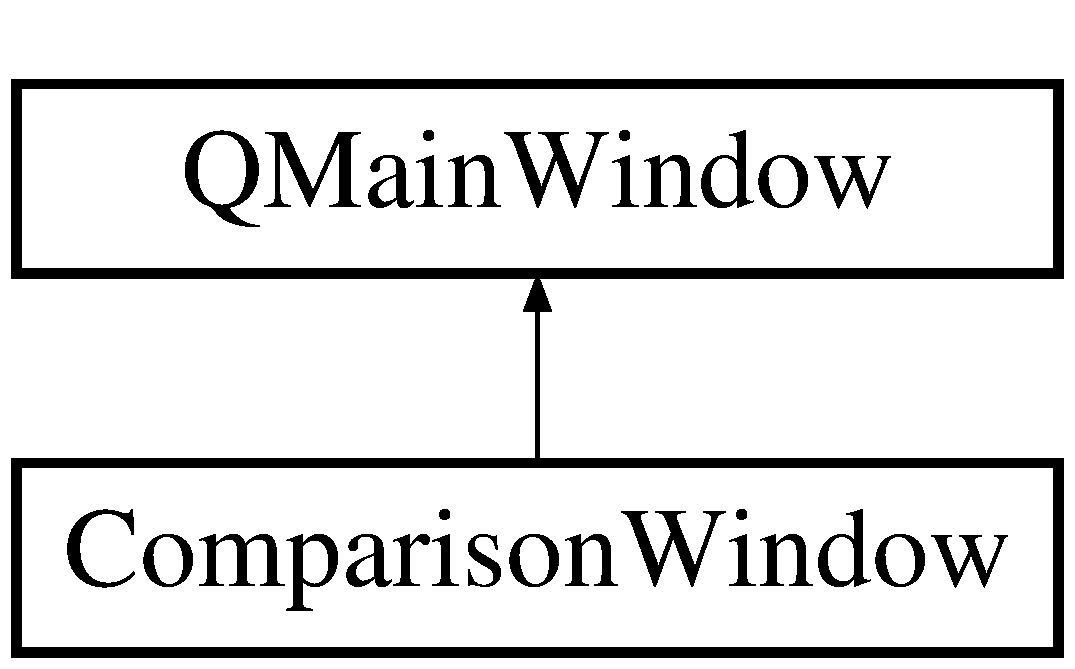
\includegraphics[height=2.000000cm]{dc/d87/class_comparison_window}
\end{center}
\end{figure}
\subsection*{Public Member Functions}
\begin{DoxyCompactItemize}
\item 
\mbox{\hyperlink{class_comparison_window_addc31fc48e96a30d630166cb377c3869}{Comparison\+Window}} (Q\+Widget $\ast$parent=0)
\begin{DoxyCompactList}\small\item\em The constructor for the \mbox{\hyperlink{class_comparison_window}{Comparison\+Window}}. \end{DoxyCompactList}\item 
\mbox{\hyperlink{class_comparison_window_a8f22c497b2b938378a4a51dc7e3ae8f2}{$\sim$\+Comparison\+Window}} ()
\begin{DoxyCompactList}\small\item\em The destructor for the comparison window. \end{DoxyCompactList}\end{DoxyCompactItemize}
\subsection*{Private Attributes}
\begin{DoxyCompactItemize}
\item 
Ui\+::\+Comparison\+Window $\ast$ \mbox{\hyperlink{class_comparison_window_a18eb77b5884a928a8b958907d1565acf}{ui}}
\begin{DoxyCompactList}\small\item\em The ui for the \mbox{\hyperlink{class_comparison_window}{Comparison\+Window}}. \end{DoxyCompactList}\end{DoxyCompactItemize}


\subsection{Detailed Description}
Contains the UI handling for the comparison window.

This class handles the various UI events that can occur on the comparison window. 

Definition at line 10 of file comparisonwindow.\+h.



\subsection{Constructor \& Destructor Documentation}
\mbox{\Hypertarget{class_comparison_window_addc31fc48e96a30d630166cb377c3869}\label{class_comparison_window_addc31fc48e96a30d630166cb377c3869}} 
\index{Comparison\+Window@{Comparison\+Window}!Comparison\+Window@{Comparison\+Window}}
\index{Comparison\+Window@{Comparison\+Window}!Comparison\+Window@{Comparison\+Window}}
\subsubsection{\texorpdfstring{Comparison\+Window()}{ComparisonWindow()}}
{\footnotesize\ttfamily Comparison\+Window\+::\+Comparison\+Window (\begin{DoxyParamCaption}\item[{Q\+Widget $\ast$}]{parent = {\ttfamily 0} }\end{DoxyParamCaption})\hspace{0.3cm}{\ttfamily [explicit]}}



The constructor for the \mbox{\hyperlink{class_comparison_window}{Comparison\+Window}}. 


\begin{DoxyParams}{Parameters}
{\em parent} & The parent widget of the \mbox{\hyperlink{class_comparison_window}{Comparison\+Window}}. \\
\hline
\end{DoxyParams}


Definition at line 20 of file comparisonwindow.\+cpp.


\begin{DoxyCode}
20                                                   :
21     QMainWindow(parent),
22     \mbox{\hyperlink{class_comparison_window_a18eb77b5884a928a8b958907d1565acf}{ui}}(\textcolor{keyword}{new} Ui::ComparisonWindow)
23 \{
24     \mbox{\hyperlink{class_comparison_window_a18eb77b5884a928a8b958907d1565acf}{ui}}->setupUi(\textcolor{keyword}{this});
25 \}
\end{DoxyCode}
\mbox{\Hypertarget{class_comparison_window_a8f22c497b2b938378a4a51dc7e3ae8f2}\label{class_comparison_window_a8f22c497b2b938378a4a51dc7e3ae8f2}} 
\index{Comparison\+Window@{Comparison\+Window}!````~Comparison\+Window@{$\sim$\+Comparison\+Window}}
\index{````~Comparison\+Window@{$\sim$\+Comparison\+Window}!Comparison\+Window@{Comparison\+Window}}
\subsubsection{\texorpdfstring{$\sim$\+Comparison\+Window()}{~ComparisonWindow()}}
{\footnotesize\ttfamily Comparison\+Window\+::$\sim$\+Comparison\+Window (\begin{DoxyParamCaption}{ }\end{DoxyParamCaption})}



The destructor for the comparison window. 



Definition at line 30 of file comparisonwindow.\+cpp.


\begin{DoxyCode}
31 \{
32     \textcolor{keyword}{delete} \mbox{\hyperlink{class_comparison_window_a18eb77b5884a928a8b958907d1565acf}{ui}};
33 \}
\end{DoxyCode}


\subsection{Member Data Documentation}
\mbox{\Hypertarget{class_comparison_window_a18eb77b5884a928a8b958907d1565acf}\label{class_comparison_window_a18eb77b5884a928a8b958907d1565acf}} 
\index{Comparison\+Window@{Comparison\+Window}!ui@{ui}}
\index{ui@{ui}!Comparison\+Window@{Comparison\+Window}}
\subsubsection{\texorpdfstring{ui}{ui}}
{\footnotesize\ttfamily Ui\+::\+Comparison\+Window$\ast$ Comparison\+Window\+::ui\hspace{0.3cm}{\ttfamily [private]}}



The ui for the \mbox{\hyperlink{class_comparison_window}{Comparison\+Window}}. 



Definition at line 19 of file comparisonwindow.\+h.



The documentation for this class was generated from the following files\+:\begin{DoxyCompactItemize}
\item 
U\+I/\mbox{\hyperlink{comparisonwindow_8h}{comparisonwindow.\+h}}\item 
U\+I/\mbox{\hyperlink{comparisonwindow_8cpp}{comparisonwindow.\+cpp}}\end{DoxyCompactItemize}

\hypertarget{class_song}{}\section{Song Class Reference}
\label{class_song}\index{Song@{Song}}


Represents a \mbox{\hyperlink{class_song}{Song}}.  




{\ttfamily \#include $<$song.\+h$>$}

Inheritance diagram for Song\+:\begin{figure}[H]
\begin{center}
\leavevmode
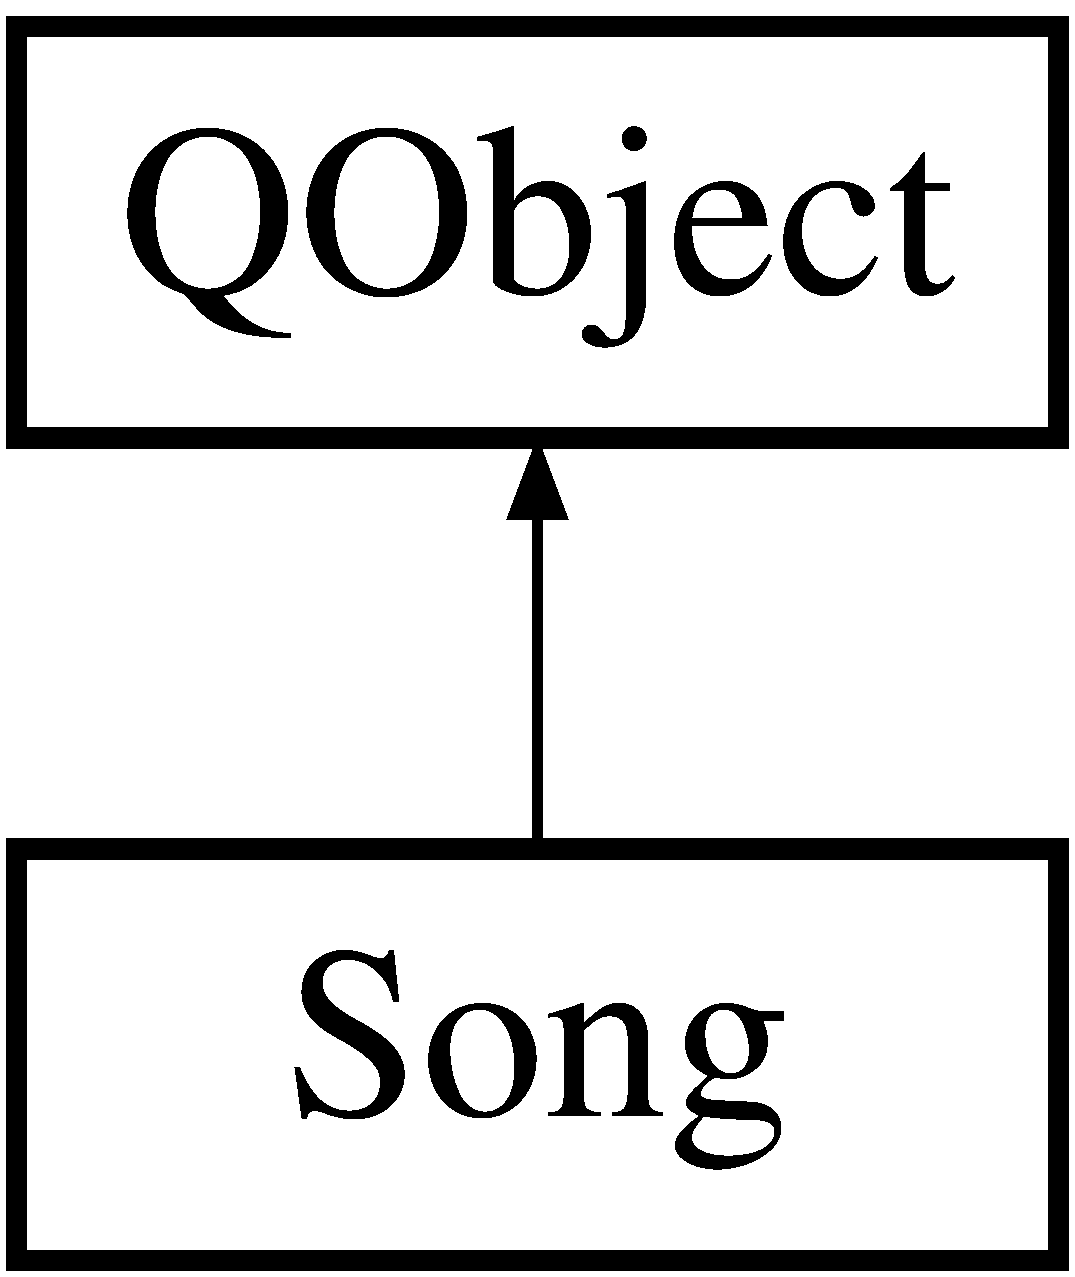
\includegraphics[height=2.000000cm]{da/dc3/class_song}
\end{center}
\end{figure}
\subsection*{Public Member Functions}
\begin{DoxyCompactItemize}
\item 
\mbox{\hyperlink{class_song_a996efbf0aa4da8315e0082107e6c6854}{Song}} (int a\+Track\+Number, Q\+String a\+Album\+Name, Q\+String a\+Artist\+Name, Q\+String a\+File\+Path, Q\+String a\+Song\+Name)
\begin{DoxyCompactList}\small\item\em Constructor for a song. \end{DoxyCompactList}\item 
\mbox{\hyperlink{class_song_a0749c3367e8de89e27458c248377027b}{$\sim$\+Song}} ()
\begin{DoxyCompactList}\small\item\em The destructor for a song. \end{DoxyCompactList}\item 
Q\+String \mbox{\hyperlink{class_song_a34913925a88e1ca698aa33af96378d2f}{get\+Album\+Name}} () const
\begin{DoxyCompactList}\small\item\em Gets the name of the album that the song belongs to. \end{DoxyCompactList}\item 
Q\+String \mbox{\hyperlink{class_song_a90ab22ea210ca1552d08f50da4c51ff5}{get\+Artist\+Name}} () const
\begin{DoxyCompactList}\small\item\em Gets the name of the artist that wrote the song. \end{DoxyCompactList}\item 
Q\+String \mbox{\hyperlink{class_song_a2c71fd5ffa7343e7688554b2f9a10120}{get\+File\+Path}} () const
\begin{DoxyCompactList}\small\item\em Gets the path to the song file. \end{DoxyCompactList}\item 
int \mbox{\hyperlink{class_song_ab80f9bd4c1b971be3daa0df1aaa2bc89}{get\+Rank}} () const
\begin{DoxyCompactList}\small\item\em Gets the ranking of the song. \end{DoxyCompactList}\item 
Q\+String \mbox{\hyperlink{class_song_a9507aeaa55d6c31f829e42432f6b5de3}{get\+Song\+Name}} () const
\begin{DoxyCompactList}\small\item\em Gets the name of the song. \end{DoxyCompactList}\item 
int \mbox{\hyperlink{class_song_aafed63304c6f308bb0c55c3ac206ad4a}{get\+Track\+Number}} () const
\begin{DoxyCompactList}\small\item\em Gets the track number of the song. \end{DoxyCompactList}\item 
void \mbox{\hyperlink{class_song_ac9c21b02ebe7a5801c2f36f255b38e49}{set\+Album\+Name}} (Q\+String a\+Album\+Name)
\begin{DoxyCompactList}\small\item\em Sets the name of the album that the song belongs to. \end{DoxyCompactList}\item 
void \mbox{\hyperlink{class_song_ab071f31965057c073c4e25a846810f8d}{set\+Artist\+Name}} (Q\+String a\+Artist\+Name)
\begin{DoxyCompactList}\small\item\em Sets the name of the artist that wrote the song. {\itshape a\+Artist\+Name} The new name of the artist that wrote the song. \end{DoxyCompactList}\item 
void \mbox{\hyperlink{class_song_ac2053f95eea7a3f96fb7d216e07637d7}{set\+File\+Path}} (Q\+String a\+File\+Path)
\begin{DoxyCompactList}\small\item\em Sets the path to the song file. {\itshape a\+File\+Path} The new file path to the song. \end{DoxyCompactList}\item 
void \mbox{\hyperlink{class_song_acbfe66b799c390ea11be07907835f057}{set\+Rank}} (int a\+Rank)
\begin{DoxyCompactList}\small\item\em Sets the ranking of the song in the sorting. {\itshape a\+Rank} The new ranking of the song. \end{DoxyCompactList}\item 
void \mbox{\hyperlink{class_song_a8ae97c3e5d99c7e8df2e1b7b4f0274ec}{set\+Song\+Name}} (Q\+String a\+Song\+Name)
\begin{DoxyCompactList}\small\item\em Sets the name of the song. {\itshape a\+Song\+Name} The new name of the song. \end{DoxyCompactList}\item 
void \mbox{\hyperlink{class_song_ab005f32d793e26e83d67132931d46769}{set\+Track\+Number}} (int a\+Track\+Number)
\begin{DoxyCompactList}\small\item\em Sets the track number of the song. \end{DoxyCompactList}\item 
bool \mbox{\hyperlink{class_song_a3e7e21ea87a93f305dbfd4cb9e6bf416}{operator$<$}} (const \mbox{\hyperlink{class_song}{Song}} \&a\+Other\+Song) const
\begin{DoxyCompactList}\small\item\em Less than operator for a \mbox{\hyperlink{class_song}{Song}}. \end{DoxyCompactList}\item 
bool \mbox{\hyperlink{class_song_a1a6cc11df009afe710a7e6103e4c4221}{operator$>$}} (const \mbox{\hyperlink{class_song}{Song}} \&a\+Other\+Song) const
\begin{DoxyCompactList}\small\item\em Greater than operator for a \mbox{\hyperlink{class_song}{Song}}. \end{DoxyCompactList}\item 
bool \mbox{\hyperlink{class_song_a3a4608e2f7744e5c1c8db350be3b24e9}{operator$<$=}} (const \mbox{\hyperlink{class_song}{Song}} \&a\+Other\+Song) const
\begin{DoxyCompactList}\small\item\em Less than or equal operator for a \mbox{\hyperlink{class_song}{Song}}. \end{DoxyCompactList}\item 
bool \mbox{\hyperlink{class_song_aa51d7041e3cb45d2e8cd3e04eac3a16f}{operator$>$=}} (const \mbox{\hyperlink{class_song}{Song}} \&a\+Other\+Song) const
\begin{DoxyCompactList}\small\item\em Greater than or equal operator for a \mbox{\hyperlink{class_song}{Song}}. \end{DoxyCompactList}\end{DoxyCompactItemize}
\subsection*{Private Attributes}
\begin{DoxyCompactItemize}
\item 
int \mbox{\hyperlink{class_song_a18b47d2545fc5e7795cad143092c97e7}{m\+Rank}}
\begin{DoxyCompactList}\small\item\em The ranking of the song in the sorting. \end{DoxyCompactList}\item 
int \mbox{\hyperlink{class_song_a45f2f019180a08117bc1992f16fdb5f7}{m\+Track\+Number}}
\begin{DoxyCompactList}\small\item\em The track number of the song in its album. \end{DoxyCompactList}\item 
Q\+String \mbox{\hyperlink{class_song_aadf3ea14887a9c5a36a1fe419d7d6222}{m\+Album\+Name}}
\begin{DoxyCompactList}\small\item\em The name of the album containing the song. \end{DoxyCompactList}\item 
Q\+String \mbox{\hyperlink{class_song_a53eb13c6325e01434ee370ba2d9af292}{m\+Artist\+Name}}
\begin{DoxyCompactList}\small\item\em The name of the artist who wrote the song. \end{DoxyCompactList}\item 
Q\+String \mbox{\hyperlink{class_song_af6852312a9369340908b7726d97979a6}{m\+File\+Path}}
\begin{DoxyCompactList}\small\item\em The file path of the song. \end{DoxyCompactList}\item 
Q\+String \mbox{\hyperlink{class_song_af7fae22fdde85f62397c5a3618e8e573}{m\+Song\+Name}}
\begin{DoxyCompactList}\small\item\em The name of the song. \end{DoxyCompactList}\end{DoxyCompactItemize}


\subsection{Detailed Description}
Represents a \mbox{\hyperlink{class_song}{Song}}. 

This class is a container that represents a \mbox{\hyperlink{class_song}{Song}} according to its metadata (artist, album, etc.) as well as its overall rank and file path. 

Definition at line 9 of file song.\+h.



\subsection{Constructor \& Destructor Documentation}
\mbox{\Hypertarget{class_song_a996efbf0aa4da8315e0082107e6c6854}\label{class_song_a996efbf0aa4da8315e0082107e6c6854}} 
\index{Song@{Song}!Song@{Song}}
\index{Song@{Song}!Song@{Song}}
\subsubsection{\texorpdfstring{Song()}{Song()}}
{\footnotesize\ttfamily Song\+::\+Song (\begin{DoxyParamCaption}\item[{int}]{a\+Track\+Number = {\ttfamily 1},  }\item[{Q\+String}]{a\+Album\+Name = {\ttfamily \char`\"{}\char`\"{}},  }\item[{Q\+String}]{a\+Artist\+Name = {\ttfamily \char`\"{}\char`\"{}},  }\item[{Q\+String}]{a\+File\+Path = {\ttfamily \char`\"{}\char`\"{}},  }\item[{Q\+String}]{a\+Song\+Name = {\ttfamily \char`\"{}\char`\"{}} }\end{DoxyParamCaption})}



Constructor for a song. 


\begin{DoxyParams}{Parameters}
{\em a\+Track\+Number} & The track number of the song. Defaults to 1. \\
\hline
{\em a\+Album\+Name} & The name of the album which the song belongs to. Defaults to an empty string. \\
\hline
{\em a\+Artist\+Name} & The name of the artist who made the song. Defaults to an empty string. \\
\hline
{\em a\+File\+Path} & The file path to the song. Defaults to an empty string. \\
\hline
{\em a\+Song\+Name} & The name of the song. Defaults to an empty string. \\
\hline
\end{DoxyParams}


Definition at line 24 of file song.\+cpp.


\begin{DoxyCode}
24                                                                                                            
                             :
25     \mbox{\hyperlink{class_song_a18b47d2545fc5e7795cad143092c97e7}{mRank}}(\mbox{\hyperlink{song_8h_a2909ea516dd5d86c56e6a2e8035fed92}{UNRANKED}}),
26     \mbox{\hyperlink{class_song_a45f2f019180a08117bc1992f16fdb5f7}{mTrackNumber}}(aTrackNumber),
27     \mbox{\hyperlink{class_song_aadf3ea14887a9c5a36a1fe419d7d6222}{mAlbumName}}(aAlbumName),
28     \mbox{\hyperlink{class_song_a53eb13c6325e01434ee370ba2d9af292}{mArtistName}}(aArtistName),
29     \mbox{\hyperlink{class_song_af6852312a9369340908b7726d97979a6}{mFilePath}}(aFilePath),
30     \mbox{\hyperlink{class_song_af7fae22fdde85f62397c5a3618e8e573}{mSongName}}(aSongName)
31 \{\}
\end{DoxyCode}
\mbox{\Hypertarget{class_song_a0749c3367e8de89e27458c248377027b}\label{class_song_a0749c3367e8de89e27458c248377027b}} 
\index{Song@{Song}!````~Song@{$\sim$\+Song}}
\index{````~Song@{$\sim$\+Song}!Song@{Song}}
\subsubsection{\texorpdfstring{$\sim$\+Song()}{~Song()}}
{\footnotesize\ttfamily Song\+::$\sim$\+Song (\begin{DoxyParamCaption}{ }\end{DoxyParamCaption})}



The destructor for a song. 



Definition at line 36 of file song.\+cpp.


\begin{DoxyCode}
37 \{\}
\end{DoxyCode}


\subsection{Member Function Documentation}
\mbox{\Hypertarget{class_song_a34913925a88e1ca698aa33af96378d2f}\label{class_song_a34913925a88e1ca698aa33af96378d2f}} 
\index{Song@{Song}!get\+Album\+Name@{get\+Album\+Name}}
\index{get\+Album\+Name@{get\+Album\+Name}!Song@{Song}}
\subsubsection{\texorpdfstring{get\+Album\+Name()}{getAlbumName()}}
{\footnotesize\ttfamily Q\+String Song\+::get\+Album\+Name (\begin{DoxyParamCaption}{ }\end{DoxyParamCaption}) const}



Gets the name of the album that the song belongs to. 

\begin{DoxyReturn}{Returns}
A Q\+String representing the name of the album that the song belongs to. 
\end{DoxyReturn}


Definition at line 47 of file song.\+cpp.


\begin{DoxyCode}
48 \{
49     \textcolor{keywordflow}{return} \mbox{\hyperlink{class_song_aadf3ea14887a9c5a36a1fe419d7d6222}{mAlbumName}};
50 \}
\end{DoxyCode}
\mbox{\Hypertarget{class_song_a90ab22ea210ca1552d08f50da4c51ff5}\label{class_song_a90ab22ea210ca1552d08f50da4c51ff5}} 
\index{Song@{Song}!get\+Artist\+Name@{get\+Artist\+Name}}
\index{get\+Artist\+Name@{get\+Artist\+Name}!Song@{Song}}
\subsubsection{\texorpdfstring{get\+Artist\+Name()}{getArtistName()}}
{\footnotesize\ttfamily Q\+String Song\+::get\+Artist\+Name (\begin{DoxyParamCaption}{ }\end{DoxyParamCaption}) const}



Gets the name of the artist that wrote the song. 

\begin{DoxyReturn}{Returns}
A Q\+String representing the name of the artist that wrote the song. 
\end{DoxyReturn}


Definition at line 56 of file song.\+cpp.


\begin{DoxyCode}
57 \{
58     \textcolor{keywordflow}{return} \mbox{\hyperlink{class_song_a53eb13c6325e01434ee370ba2d9af292}{mArtistName}};
59 \}
\end{DoxyCode}
\mbox{\Hypertarget{class_song_a2c71fd5ffa7343e7688554b2f9a10120}\label{class_song_a2c71fd5ffa7343e7688554b2f9a10120}} 
\index{Song@{Song}!get\+File\+Path@{get\+File\+Path}}
\index{get\+File\+Path@{get\+File\+Path}!Song@{Song}}
\subsubsection{\texorpdfstring{get\+File\+Path()}{getFilePath()}}
{\footnotesize\ttfamily Q\+String Song\+::get\+File\+Path (\begin{DoxyParamCaption}{ }\end{DoxyParamCaption}) const}



Gets the path to the song file. 

\begin{DoxyReturn}{Returns}
A Q\+String representing the file path of the song. 
\end{DoxyReturn}


Definition at line 65 of file song.\+cpp.


\begin{DoxyCode}
66 \{
67     \textcolor{keywordflow}{return} \mbox{\hyperlink{class_song_af6852312a9369340908b7726d97979a6}{mFilePath}};
68 \}
\end{DoxyCode}
\mbox{\Hypertarget{class_song_ab80f9bd4c1b971be3daa0df1aaa2bc89}\label{class_song_ab80f9bd4c1b971be3daa0df1aaa2bc89}} 
\index{Song@{Song}!get\+Rank@{get\+Rank}}
\index{get\+Rank@{get\+Rank}!Song@{Song}}
\subsubsection{\texorpdfstring{get\+Rank()}{getRank()}}
{\footnotesize\ttfamily int Song\+::get\+Rank (\begin{DoxyParamCaption}{ }\end{DoxyParamCaption}) const}



Gets the ranking of the song. 

\begin{DoxyReturn}{Returns}
An integer representing the ranking of the song in the sorting. 
\end{DoxyReturn}


Definition at line 74 of file song.\+cpp.


\begin{DoxyCode}
75 \{
76     \textcolor{keywordflow}{return} \mbox{\hyperlink{class_song_a18b47d2545fc5e7795cad143092c97e7}{mRank}};
77 \}
\end{DoxyCode}
\mbox{\Hypertarget{class_song_a9507aeaa55d6c31f829e42432f6b5de3}\label{class_song_a9507aeaa55d6c31f829e42432f6b5de3}} 
\index{Song@{Song}!get\+Song\+Name@{get\+Song\+Name}}
\index{get\+Song\+Name@{get\+Song\+Name}!Song@{Song}}
\subsubsection{\texorpdfstring{get\+Song\+Name()}{getSongName()}}
{\footnotesize\ttfamily Q\+String Song\+::get\+Song\+Name (\begin{DoxyParamCaption}{ }\end{DoxyParamCaption}) const}



Gets the name of the song. 

\begin{DoxyReturn}{Returns}
A Q\+String representing the name of song. 
\end{DoxyReturn}


Definition at line 83 of file song.\+cpp.


\begin{DoxyCode}
84 \{
85     \textcolor{keywordflow}{return} \mbox{\hyperlink{class_song_af7fae22fdde85f62397c5a3618e8e573}{mSongName}};
86 \}
\end{DoxyCode}
\mbox{\Hypertarget{class_song_aafed63304c6f308bb0c55c3ac206ad4a}\label{class_song_aafed63304c6f308bb0c55c3ac206ad4a}} 
\index{Song@{Song}!get\+Track\+Number@{get\+Track\+Number}}
\index{get\+Track\+Number@{get\+Track\+Number}!Song@{Song}}
\subsubsection{\texorpdfstring{get\+Track\+Number()}{getTrackNumber()}}
{\footnotesize\ttfamily int Song\+::get\+Track\+Number (\begin{DoxyParamCaption}{ }\end{DoxyParamCaption}) const}



Gets the track number of the song. 

\begin{DoxyReturn}{Returns}
An integer representing the track number of the song. 
\end{DoxyReturn}


Definition at line 92 of file song.\+cpp.


\begin{DoxyCode}
93 \{
94     \textcolor{keywordflow}{return} \mbox{\hyperlink{class_song_a45f2f019180a08117bc1992f16fdb5f7}{mTrackNumber}};
95 \}
\end{DoxyCode}
\mbox{\Hypertarget{class_song_a3e7e21ea87a93f305dbfd4cb9e6bf416}\label{class_song_a3e7e21ea87a93f305dbfd4cb9e6bf416}} 
\index{Song@{Song}!operator$<$@{operator$<$}}
\index{operator$<$@{operator$<$}!Song@{Song}}
\subsubsection{\texorpdfstring{operator$<$()}{operator<()}}
{\footnotesize\ttfamily bool Song\+::operator$<$ (\begin{DoxyParamCaption}\item[{const \mbox{\hyperlink{class_song}{Song}} \&}]{a\+Other\+Song }\end{DoxyParamCaption}) const}



Less than operator for a \mbox{\hyperlink{class_song}{Song}}. 


\begin{DoxyParams}{Parameters}
{\em a\+Other\+Song} & The song to compare to this one. \\
\hline
\end{DoxyParams}
\begin{DoxyReturn}{Returns}
True if this \mbox{\hyperlink{class_song}{Song}}\textquotesingle{}s rank is less than a\+Other\+Song\textquotesingle{}s rank. 
\end{DoxyReturn}


Definition at line 164 of file song.\+cpp.


\begin{DoxyCode}
165 \{
166     \textcolor{keywordflow}{return} \mbox{\hyperlink{class_song_a18b47d2545fc5e7795cad143092c97e7}{mRank}} < aOtherSong.\mbox{\hyperlink{class_song_a18b47d2545fc5e7795cad143092c97e7}{mRank}};
167 \}
\end{DoxyCode}
\mbox{\Hypertarget{class_song_a3a4608e2f7744e5c1c8db350be3b24e9}\label{class_song_a3a4608e2f7744e5c1c8db350be3b24e9}} 
\index{Song@{Song}!operator$<$=@{operator$<$=}}
\index{operator$<$=@{operator$<$=}!Song@{Song}}
\subsubsection{\texorpdfstring{operator$<$=()}{operator<=()}}
{\footnotesize\ttfamily bool Song\+::operator$<$= (\begin{DoxyParamCaption}\item[{const \mbox{\hyperlink{class_song}{Song}} \&}]{a\+Other\+Song }\end{DoxyParamCaption}) const}



Less than or equal operator for a \mbox{\hyperlink{class_song}{Song}}. 


\begin{DoxyParams}{Parameters}
{\em a\+Other\+Song} & The song to compare to this one. \\
\hline
\end{DoxyParams}
\begin{DoxyReturn}{Returns}
True if this \mbox{\hyperlink{class_song}{Song}}\textquotesingle{}s rank is less than or equal to a\+Other\+Song\textquotesingle{}s rank. 
\end{DoxyReturn}


Definition at line 184 of file song.\+cpp.


\begin{DoxyCode}
185 \{
186     \textcolor{keywordflow}{return} \mbox{\hyperlink{class_song_a18b47d2545fc5e7795cad143092c97e7}{mRank}} <= aOtherSong.\mbox{\hyperlink{class_song_a18b47d2545fc5e7795cad143092c97e7}{mRank}};
187 \}
\end{DoxyCode}
\mbox{\Hypertarget{class_song_a1a6cc11df009afe710a7e6103e4c4221}\label{class_song_a1a6cc11df009afe710a7e6103e4c4221}} 
\index{Song@{Song}!operator$>$@{operator$>$}}
\index{operator$>$@{operator$>$}!Song@{Song}}
\subsubsection{\texorpdfstring{operator$>$()}{operator>()}}
{\footnotesize\ttfamily bool Song\+::operator$>$ (\begin{DoxyParamCaption}\item[{const \mbox{\hyperlink{class_song}{Song}} \&}]{a\+Other\+Song }\end{DoxyParamCaption}) const}



Greater than operator for a \mbox{\hyperlink{class_song}{Song}}. 


\begin{DoxyParams}{Parameters}
{\em a\+Other\+Song} & The song to compare to this one. \\
\hline
\end{DoxyParams}
\begin{DoxyReturn}{Returns}
True if this \mbox{\hyperlink{class_song}{Song}}\textquotesingle{}s rank is greater than a\+Other\+Song\textquotesingle{}s rank. 
\end{DoxyReturn}


Definition at line 174 of file song.\+cpp.


\begin{DoxyCode}
175 \{
176     \textcolor{keywordflow}{return} \mbox{\hyperlink{class_song_a18b47d2545fc5e7795cad143092c97e7}{mRank}} > aOtherSong.\mbox{\hyperlink{class_song_a18b47d2545fc5e7795cad143092c97e7}{mRank}};
177 \}
\end{DoxyCode}
\mbox{\Hypertarget{class_song_aa51d7041e3cb45d2e8cd3e04eac3a16f}\label{class_song_aa51d7041e3cb45d2e8cd3e04eac3a16f}} 
\index{Song@{Song}!operator$>$=@{operator$>$=}}
\index{operator$>$=@{operator$>$=}!Song@{Song}}
\subsubsection{\texorpdfstring{operator$>$=()}{operator>=()}}
{\footnotesize\ttfamily bool Song\+::operator$>$= (\begin{DoxyParamCaption}\item[{const \mbox{\hyperlink{class_song}{Song}} \&}]{a\+Other\+Song }\end{DoxyParamCaption}) const}



Greater than or equal operator for a \mbox{\hyperlink{class_song}{Song}}. 


\begin{DoxyParams}{Parameters}
{\em a\+Other\+Song} & The song to compare to this one. \\
\hline
\end{DoxyParams}
\begin{DoxyReturn}{Returns}
True if this \mbox{\hyperlink{class_song}{Song}}\textquotesingle{}s rank is greater than or equal to a\+Other\+Song\textquotesingle{}s rank. 
\end{DoxyReturn}


Definition at line 194 of file song.\+cpp.


\begin{DoxyCode}
195 \{
196     \textcolor{keywordflow}{return} \mbox{\hyperlink{class_song_a18b47d2545fc5e7795cad143092c97e7}{mRank}} >= aOtherSong.\mbox{\hyperlink{class_song_a18b47d2545fc5e7795cad143092c97e7}{mRank}};
197 \}
\end{DoxyCode}
\mbox{\Hypertarget{class_song_ac9c21b02ebe7a5801c2f36f255b38e49}\label{class_song_ac9c21b02ebe7a5801c2f36f255b38e49}} 
\index{Song@{Song}!set\+Album\+Name@{set\+Album\+Name}}
\index{set\+Album\+Name@{set\+Album\+Name}!Song@{Song}}
\subsubsection{\texorpdfstring{set\+Album\+Name()}{setAlbumName()}}
{\footnotesize\ttfamily void Song\+::set\+Album\+Name (\begin{DoxyParamCaption}\item[{Q\+String}]{a\+Album\+Name }\end{DoxyParamCaption})}



Sets the name of the album that the song belongs to. 


\begin{DoxyParams}{Parameters}
{\em a\+Album\+Name} & The new name of the album that the song belongs to. \\
\hline
\end{DoxyParams}


Definition at line 101 of file song.\+cpp.


\begin{DoxyCode}
102 \{
103     \mbox{\hyperlink{class_song_aadf3ea14887a9c5a36a1fe419d7d6222}{mAlbumName}} = aAlbumName;
104 \}
\end{DoxyCode}
\mbox{\Hypertarget{class_song_ab071f31965057c073c4e25a846810f8d}\label{class_song_ab071f31965057c073c4e25a846810f8d}} 
\index{Song@{Song}!set\+Artist\+Name@{set\+Artist\+Name}}
\index{set\+Artist\+Name@{set\+Artist\+Name}!Song@{Song}}
\subsubsection{\texorpdfstring{set\+Artist\+Name()}{setArtistName()}}
{\footnotesize\ttfamily void Song\+::set\+Artist\+Name (\begin{DoxyParamCaption}\item[{Q\+String}]{a\+Artist\+Name }\end{DoxyParamCaption})}



Sets the name of the artist that wrote the song. {\itshape a\+Artist\+Name} The new name of the artist that wrote the song. 



Definition at line 111 of file song.\+cpp.


\begin{DoxyCode}
112 \{
113     \mbox{\hyperlink{class_song_a53eb13c6325e01434ee370ba2d9af292}{mArtistName}} = aArtistName;
114 \}
\end{DoxyCode}
\mbox{\Hypertarget{class_song_ac2053f95eea7a3f96fb7d216e07637d7}\label{class_song_ac2053f95eea7a3f96fb7d216e07637d7}} 
\index{Song@{Song}!set\+File\+Path@{set\+File\+Path}}
\index{set\+File\+Path@{set\+File\+Path}!Song@{Song}}
\subsubsection{\texorpdfstring{set\+File\+Path()}{setFilePath()}}
{\footnotesize\ttfamily void Song\+::set\+File\+Path (\begin{DoxyParamCaption}\item[{Q\+String}]{a\+File\+Path }\end{DoxyParamCaption})}



Sets the path to the song file. {\itshape a\+File\+Path} The new file path to the song. 



Definition at line 121 of file song.\+cpp.


\begin{DoxyCode}
122 \{
123     \mbox{\hyperlink{class_song_af6852312a9369340908b7726d97979a6}{mFilePath}} = aFilePath;
124 \}
\end{DoxyCode}
\mbox{\Hypertarget{class_song_acbfe66b799c390ea11be07907835f057}\label{class_song_acbfe66b799c390ea11be07907835f057}} 
\index{Song@{Song}!set\+Rank@{set\+Rank}}
\index{set\+Rank@{set\+Rank}!Song@{Song}}
\subsubsection{\texorpdfstring{set\+Rank()}{setRank()}}
{\footnotesize\ttfamily void Song\+::set\+Rank (\begin{DoxyParamCaption}\item[{int}]{a\+Rank }\end{DoxyParamCaption})}



Sets the ranking of the song in the sorting. {\itshape a\+Rank} The new ranking of the song. 



Definition at line 131 of file song.\+cpp.


\begin{DoxyCode}
132 \{
133     \mbox{\hyperlink{class_song_a18b47d2545fc5e7795cad143092c97e7}{mRank}} = aRank;
134 \}
\end{DoxyCode}
\mbox{\Hypertarget{class_song_a8ae97c3e5d99c7e8df2e1b7b4f0274ec}\label{class_song_a8ae97c3e5d99c7e8df2e1b7b4f0274ec}} 
\index{Song@{Song}!set\+Song\+Name@{set\+Song\+Name}}
\index{set\+Song\+Name@{set\+Song\+Name}!Song@{Song}}
\subsubsection{\texorpdfstring{set\+Song\+Name()}{setSongName()}}
{\footnotesize\ttfamily void Song\+::set\+Song\+Name (\begin{DoxyParamCaption}\item[{Q\+String}]{a\+Song\+Name }\end{DoxyParamCaption})}



Sets the name of the song. {\itshape a\+Song\+Name} The new name of the song. 



Definition at line 141 of file song.\+cpp.


\begin{DoxyCode}
142 \{
143     \mbox{\hyperlink{class_song_af7fae22fdde85f62397c5a3618e8e573}{mSongName}} = aSongName;
144 \}
\end{DoxyCode}
\mbox{\Hypertarget{class_song_ab005f32d793e26e83d67132931d46769}\label{class_song_ab005f32d793e26e83d67132931d46769}} 
\index{Song@{Song}!set\+Track\+Number@{set\+Track\+Number}}
\index{set\+Track\+Number@{set\+Track\+Number}!Song@{Song}}
\subsubsection{\texorpdfstring{set\+Track\+Number()}{setTrackNumber()}}
{\footnotesize\ttfamily void Song\+::set\+Track\+Number (\begin{DoxyParamCaption}\item[{int}]{a\+Track\+Number }\end{DoxyParamCaption})}



Sets the track number of the song. 


\begin{DoxyParams}{Parameters}
{\em a\+Track\+Number} & The new track number of the song. \\
\hline
\end{DoxyParams}


Definition at line 150 of file song.\+cpp.


\begin{DoxyCode}
151 \{
152     \mbox{\hyperlink{class_song_a45f2f019180a08117bc1992f16fdb5f7}{mTrackNumber}} = aTrackNumber;
153 \}
\end{DoxyCode}


\subsection{Member Data Documentation}
\mbox{\Hypertarget{class_song_aadf3ea14887a9c5a36a1fe419d7d6222}\label{class_song_aadf3ea14887a9c5a36a1fe419d7d6222}} 
\index{Song@{Song}!m\+Album\+Name@{m\+Album\+Name}}
\index{m\+Album\+Name@{m\+Album\+Name}!Song@{Song}}
\subsubsection{\texorpdfstring{m\+Album\+Name}{mAlbumName}}
{\footnotesize\ttfamily Q\+String Song\+::m\+Album\+Name\hspace{0.3cm}{\ttfamily [private]}}



The name of the album containing the song. 



Definition at line 38 of file song.\+h.

\mbox{\Hypertarget{class_song_a53eb13c6325e01434ee370ba2d9af292}\label{class_song_a53eb13c6325e01434ee370ba2d9af292}} 
\index{Song@{Song}!m\+Artist\+Name@{m\+Artist\+Name}}
\index{m\+Artist\+Name@{m\+Artist\+Name}!Song@{Song}}
\subsubsection{\texorpdfstring{m\+Artist\+Name}{mArtistName}}
{\footnotesize\ttfamily Q\+String Song\+::m\+Artist\+Name\hspace{0.3cm}{\ttfamily [private]}}



The name of the artist who wrote the song. 



Definition at line 39 of file song.\+h.

\mbox{\Hypertarget{class_song_af6852312a9369340908b7726d97979a6}\label{class_song_af6852312a9369340908b7726d97979a6}} 
\index{Song@{Song}!m\+File\+Path@{m\+File\+Path}}
\index{m\+File\+Path@{m\+File\+Path}!Song@{Song}}
\subsubsection{\texorpdfstring{m\+File\+Path}{mFilePath}}
{\footnotesize\ttfamily Q\+String Song\+::m\+File\+Path\hspace{0.3cm}{\ttfamily [private]}}



The file path of the song. 



Definition at line 40 of file song.\+h.

\mbox{\Hypertarget{class_song_a18b47d2545fc5e7795cad143092c97e7}\label{class_song_a18b47d2545fc5e7795cad143092c97e7}} 
\index{Song@{Song}!m\+Rank@{m\+Rank}}
\index{m\+Rank@{m\+Rank}!Song@{Song}}
\subsubsection{\texorpdfstring{m\+Rank}{mRank}}
{\footnotesize\ttfamily int Song\+::m\+Rank\hspace{0.3cm}{\ttfamily [private]}}



The ranking of the song in the sorting. 



Definition at line 36 of file song.\+h.

\mbox{\Hypertarget{class_song_af7fae22fdde85f62397c5a3618e8e573}\label{class_song_af7fae22fdde85f62397c5a3618e8e573}} 
\index{Song@{Song}!m\+Song\+Name@{m\+Song\+Name}}
\index{m\+Song\+Name@{m\+Song\+Name}!Song@{Song}}
\subsubsection{\texorpdfstring{m\+Song\+Name}{mSongName}}
{\footnotesize\ttfamily Q\+String Song\+::m\+Song\+Name\hspace{0.3cm}{\ttfamily [private]}}



The name of the song. 



Definition at line 41 of file song.\+h.

\mbox{\Hypertarget{class_song_a45f2f019180a08117bc1992f16fdb5f7}\label{class_song_a45f2f019180a08117bc1992f16fdb5f7}} 
\index{Song@{Song}!m\+Track\+Number@{m\+Track\+Number}}
\index{m\+Track\+Number@{m\+Track\+Number}!Song@{Song}}
\subsubsection{\texorpdfstring{m\+Track\+Number}{mTrackNumber}}
{\footnotesize\ttfamily int Song\+::m\+Track\+Number\hspace{0.3cm}{\ttfamily [private]}}



The track number of the song in its album. 



Definition at line 37 of file song.\+h.



The documentation for this class was generated from the following files\+:\begin{DoxyCompactItemize}
\item 
song\+Handling/\mbox{\hyperlink{song_8h}{song.\+h}}\item 
song\+Handling/\mbox{\hyperlink{song_8cpp}{song.\+cpp}}\end{DoxyCompactItemize}

\hypertarget{struct_song_list_viewer_window_1_1song__edit}{}\section{Song\+List\+Viewer\+Window\+:\+:song\+\_\+edit Struct Reference}
\label{struct_song_list_viewer_window_1_1song__edit}\index{Song\+List\+Viewer\+Window\+::song\+\_\+edit@{Song\+List\+Viewer\+Window\+::song\+\_\+edit}}


Keeps tracks of edits that occur to a song in the table.  


\subsection*{Public Attributes}
\begin{DoxyCompactItemize}
\item 
bool \mbox{\hyperlink{struct_song_list_viewer_window_1_1song__edit_ac10b306fd227c9b4f36a0c9d41f4e5ed}{remove\+\_\+song}} = false
\begin{DoxyCompactList}\small\item\em True if the \mbox{\hyperlink{class_song}{Song}} should not be imported. \end{DoxyCompactList}\item 
bool \mbox{\hyperlink{struct_song_list_viewer_window_1_1song__edit_ac5afb4d077978f41b62842de638ab60c}{artist\+\_\+edited}} = false
\begin{DoxyCompactList}\small\item\em True if the artist of the \mbox{\hyperlink{class_song}{Song}} was edited. \end{DoxyCompactList}\item 
bool \mbox{\hyperlink{struct_song_list_viewer_window_1_1song__edit_ac78cf078f8fb2fb5d482c80cff7bc860}{album\+\_\+edited}} = false
\begin{DoxyCompactList}\small\item\em True if the name of the album containing the \mbox{\hyperlink{class_song}{Song}} was edited. \end{DoxyCompactList}\item 
bool \mbox{\hyperlink{struct_song_list_viewer_window_1_1song__edit_ac26e42f1a25121026d3eb57eb9f141e1}{track\+\_\+number\+\_\+edited}} = false
\begin{DoxyCompactList}\small\item\em True if the track number of the \mbox{\hyperlink{class_song}{Song}} was edited. \end{DoxyCompactList}\item 
bool \mbox{\hyperlink{struct_song_list_viewer_window_1_1song__edit_a15419ad06dd36c199d9e41debc3072f7}{song\+\_\+name\+\_\+edited}} = false
\begin{DoxyCompactList}\small\item\em True if the name of the \mbox{\hyperlink{class_song}{Song}} was edited. \end{DoxyCompactList}\end{DoxyCompactItemize}


\subsection{Detailed Description}
Keeps tracks of edits that occur to a song in the table. 

Definition at line 65 of file songlistviewerwindow.\+h.



\subsection{Member Data Documentation}
\mbox{\Hypertarget{struct_song_list_viewer_window_1_1song__edit_ac78cf078f8fb2fb5d482c80cff7bc860}\label{struct_song_list_viewer_window_1_1song__edit_ac78cf078f8fb2fb5d482c80cff7bc860}} 
\index{Song\+List\+Viewer\+Window\+::song\+\_\+edit@{Song\+List\+Viewer\+Window\+::song\+\_\+edit}!album\+\_\+edited@{album\+\_\+edited}}
\index{album\+\_\+edited@{album\+\_\+edited}!Song\+List\+Viewer\+Window\+::song\+\_\+edit@{Song\+List\+Viewer\+Window\+::song\+\_\+edit}}
\subsubsection{\texorpdfstring{album\+\_\+edited}{album\_edited}}
{\footnotesize\ttfamily bool Song\+List\+Viewer\+Window\+::song\+\_\+edit\+::album\+\_\+edited = false}



True if the name of the album containing the \mbox{\hyperlink{class_song}{Song}} was edited. 



Definition at line 69 of file songlistviewerwindow.\+h.

\mbox{\Hypertarget{struct_song_list_viewer_window_1_1song__edit_ac5afb4d077978f41b62842de638ab60c}\label{struct_song_list_viewer_window_1_1song__edit_ac5afb4d077978f41b62842de638ab60c}} 
\index{Song\+List\+Viewer\+Window\+::song\+\_\+edit@{Song\+List\+Viewer\+Window\+::song\+\_\+edit}!artist\+\_\+edited@{artist\+\_\+edited}}
\index{artist\+\_\+edited@{artist\+\_\+edited}!Song\+List\+Viewer\+Window\+::song\+\_\+edit@{Song\+List\+Viewer\+Window\+::song\+\_\+edit}}
\subsubsection{\texorpdfstring{artist\+\_\+edited}{artist\_edited}}
{\footnotesize\ttfamily bool Song\+List\+Viewer\+Window\+::song\+\_\+edit\+::artist\+\_\+edited = false}



True if the artist of the \mbox{\hyperlink{class_song}{Song}} was edited. 



Definition at line 68 of file songlistviewerwindow.\+h.

\mbox{\Hypertarget{struct_song_list_viewer_window_1_1song__edit_ac10b306fd227c9b4f36a0c9d41f4e5ed}\label{struct_song_list_viewer_window_1_1song__edit_ac10b306fd227c9b4f36a0c9d41f4e5ed}} 
\index{Song\+List\+Viewer\+Window\+::song\+\_\+edit@{Song\+List\+Viewer\+Window\+::song\+\_\+edit}!remove\+\_\+song@{remove\+\_\+song}}
\index{remove\+\_\+song@{remove\+\_\+song}!Song\+List\+Viewer\+Window\+::song\+\_\+edit@{Song\+List\+Viewer\+Window\+::song\+\_\+edit}}
\subsubsection{\texorpdfstring{remove\+\_\+song}{remove\_song}}
{\footnotesize\ttfamily bool Song\+List\+Viewer\+Window\+::song\+\_\+edit\+::remove\+\_\+song = false}



True if the \mbox{\hyperlink{class_song}{Song}} should not be imported. 



Definition at line 67 of file songlistviewerwindow.\+h.

\mbox{\Hypertarget{struct_song_list_viewer_window_1_1song__edit_a15419ad06dd36c199d9e41debc3072f7}\label{struct_song_list_viewer_window_1_1song__edit_a15419ad06dd36c199d9e41debc3072f7}} 
\index{Song\+List\+Viewer\+Window\+::song\+\_\+edit@{Song\+List\+Viewer\+Window\+::song\+\_\+edit}!song\+\_\+name\+\_\+edited@{song\+\_\+name\+\_\+edited}}
\index{song\+\_\+name\+\_\+edited@{song\+\_\+name\+\_\+edited}!Song\+List\+Viewer\+Window\+::song\+\_\+edit@{Song\+List\+Viewer\+Window\+::song\+\_\+edit}}
\subsubsection{\texorpdfstring{song\+\_\+name\+\_\+edited}{song\_name\_edited}}
{\footnotesize\ttfamily bool Song\+List\+Viewer\+Window\+::song\+\_\+edit\+::song\+\_\+name\+\_\+edited = false}



True if the name of the \mbox{\hyperlink{class_song}{Song}} was edited. 



Definition at line 71 of file songlistviewerwindow.\+h.

\mbox{\Hypertarget{struct_song_list_viewer_window_1_1song__edit_ac26e42f1a25121026d3eb57eb9f141e1}\label{struct_song_list_viewer_window_1_1song__edit_ac26e42f1a25121026d3eb57eb9f141e1}} 
\index{Song\+List\+Viewer\+Window\+::song\+\_\+edit@{Song\+List\+Viewer\+Window\+::song\+\_\+edit}!track\+\_\+number\+\_\+edited@{track\+\_\+number\+\_\+edited}}
\index{track\+\_\+number\+\_\+edited@{track\+\_\+number\+\_\+edited}!Song\+List\+Viewer\+Window\+::song\+\_\+edit@{Song\+List\+Viewer\+Window\+::song\+\_\+edit}}
\subsubsection{\texorpdfstring{track\+\_\+number\+\_\+edited}{track\_number\_edited}}
{\footnotesize\ttfamily bool Song\+List\+Viewer\+Window\+::song\+\_\+edit\+::track\+\_\+number\+\_\+edited = false}



True if the track number of the \mbox{\hyperlink{class_song}{Song}} was edited. 



Definition at line 70 of file songlistviewerwindow.\+h.



The documentation for this struct was generated from the following file\+:\begin{DoxyCompactItemize}
\item 
U\+I/\mbox{\hyperlink{songlistviewerwindow_8h}{songlistviewerwindow.\+h}}\end{DoxyCompactItemize}

\hypertarget{class_song_list_viewer_window}{}\section{Song\+List\+Viewer\+Window Class Reference}
\label{class_song_list_viewer_window}\index{Song\+List\+Viewer\+Window@{Song\+List\+Viewer\+Window}}


Allows the user to choose which songs to import from a folder.

This class implements event handling for a window that displays lists of \mbox{\hyperlink{class_song}{songs}}. The window has different \mbox{\hyperlink{class_song_list_viewer_window_a6f23a68c416173f6b571a2cc4990a927}{modes}} that it can be run in, and these modes dictate the actions that are available for the user in the window.  




{\ttfamily \#include $<$songlistviewerwindow.\+h$>$}

Inheritance diagram for Song\+List\+Viewer\+Window\+:\begin{figure}[H]
\begin{center}
\leavevmode
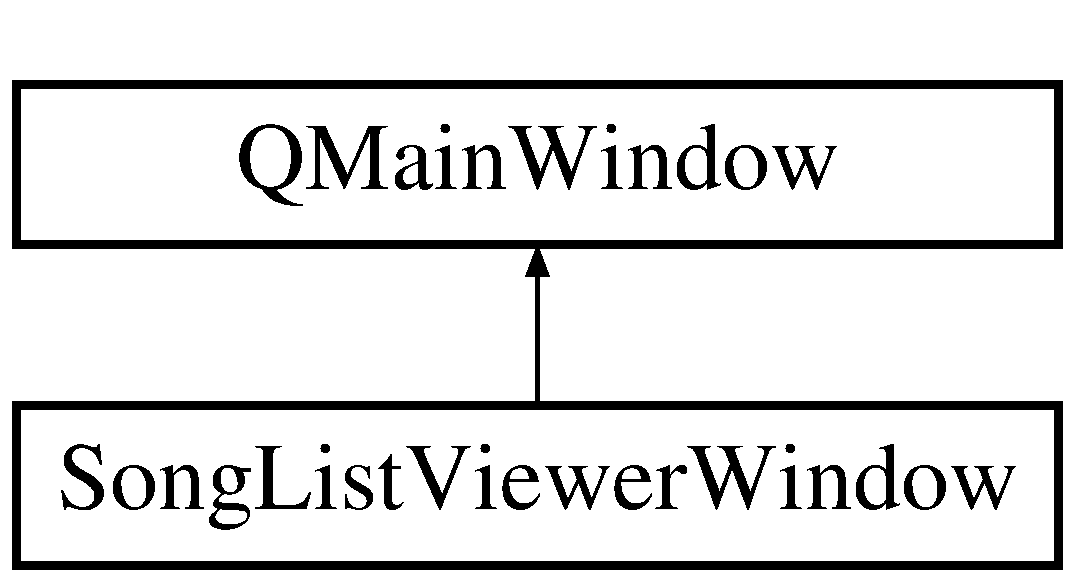
\includegraphics[height=2.000000cm]{da/dcb/class_song_list_viewer_window}
\end{center}
\end{figure}
\subsection*{Classes}
\begin{DoxyCompactItemize}
\item 
struct \mbox{\hyperlink{struct_song_list_viewer_window_1_1song__edit}{song\+\_\+edit}}
\begin{DoxyCompactList}\small\item\em Keeps tracks of edits that occur to a song in the table. \end{DoxyCompactList}\end{DoxyCompactItemize}
\subsection*{Public Types}
\begin{DoxyCompactItemize}
\item 
enum \mbox{\hyperlink{class_song_list_viewer_window_a6f23a68c416173f6b571a2cc4990a927}{S\+O\+N\+G\+\_\+\+L\+I\+S\+T\+\_\+\+M\+O\+DE}} \{ \mbox{\hyperlink{class_song_list_viewer_window_a6f23a68c416173f6b571a2cc4990a927a9847037eeae7688b9cddf8700d425332}{C\+O\+N\+F\+I\+R\+M\+\_\+\+I\+M\+P\+O\+R\+T\+E\+D\+\_\+\+S\+O\+N\+GS}}, 
\mbox{\hyperlink{class_song_list_viewer_window_a6f23a68c416173f6b571a2cc4990a927ad119fc74405f78aff7ed2efda3eb7b74}{E\+D\+I\+T\+\_\+\+M\+A\+I\+N\+\_\+\+S\+O\+N\+G\+\_\+\+L\+I\+ST}}, 
\mbox{\hyperlink{class_song_list_viewer_window_a6f23a68c416173f6b571a2cc4990a927a7fbcaf0d5c1145332e50928f877040b4}{S\+H\+O\+W\+\_\+\+R\+E\+S\+U\+L\+TS}}
 \}
\begin{DoxyCompactList}\small\item\em The different modes of the \mbox{\hyperlink{class_song_list_viewer_window}{Song\+List\+Viewer\+Window}}. \end{DoxyCompactList}\item 
typedef enum \mbox{\hyperlink{class_song_list_viewer_window_a6f23a68c416173f6b571a2cc4990a927}{Song\+List\+Viewer\+Window\+::\+S\+O\+N\+G\+\_\+\+L\+I\+S\+T\+\_\+\+M\+O\+DE}} \mbox{\hyperlink{class_song_list_viewer_window_a2942818cc26b8ff9e29827f97356ac9c}{S\+O\+N\+G\+\_\+\+L\+I\+S\+T\+\_\+\+M\+O\+DE}}
\begin{DoxyCompactList}\small\item\em The different modes of the \mbox{\hyperlink{class_song_list_viewer_window}{Song\+List\+Viewer\+Window}}. \end{DoxyCompactList}\end{DoxyCompactItemize}
\subsection*{Signals}
\begin{DoxyCompactItemize}
\item 
void \mbox{\hyperlink{class_song_list_viewer_window_a2f54dad3e714cd08fd85080a8865f616}{import\+Cancelled}} ()
\begin{DoxyCompactList}\small\item\em Emitted when the window exits with unsaved changes. \end{DoxyCompactList}\item 
void \mbox{\hyperlink{class_song_list_viewer_window_a72159650ecd17b063a01c97b38c9c3c4}{imported\+Songs\+Confirmed}} ()
\begin{DoxyCompactList}\small\item\em Emitted when songs imported from a folder have been confirmed for inclusion in the sort. \end{DoxyCompactList}\item 
void \mbox{\hyperlink{class_song_list_viewer_window_a6fb4b39cdd5f7b9a3f8b12bcb2ec4c35}{song\+List\+Edited}} ()
\begin{DoxyCompactList}\small\item\em Emitted when the main \mbox{\hyperlink{class_song}{Song}} list has been edited. \end{DoxyCompactList}\item 
void \mbox{\hyperlink{class_song_list_viewer_window_aa87ae7b7b4d0620111303d1cad334320}{results\+Window\+Closed}} ()
\begin{DoxyCompactList}\small\item\em Emitted when the window exits when it is displaying the results of the sort. \end{DoxyCompactList}\end{DoxyCompactItemize}
\subsection*{Public Member Functions}
\begin{DoxyCompactItemize}
\item 
\mbox{\hyperlink{class_song_list_viewer_window_a5691d305c3ccaeea7e0213c1722c5c38}{Song\+List\+Viewer\+Window}} (Q\+Widget $\ast$parent=0)
\begin{DoxyCompactList}\small\item\em Constructor for the \mbox{\hyperlink{class_song_list_viewer_window}{Song\+List\+Viewer\+Window}}. \end{DoxyCompactList}\item 
\mbox{\hyperlink{class_song_list_viewer_window_a563ac79baf2458f7f33c961fb433541d}{$\sim$\+Song\+List\+Viewer\+Window}} ()
\begin{DoxyCompactList}\small\item\em Destructor for the \mbox{\hyperlink{class_song_list_viewer_window}{Song\+List\+Viewer\+Window}}. \end{DoxyCompactList}\item 
void \mbox{\hyperlink{class_song_list_viewer_window_ae26127c85ed57885461c5143be4ae1e9}{setup\+Song\+List\+Viewer\+Window}} (\mbox{\hyperlink{class_song_list_viewer_window_a6f23a68c416173f6b571a2cc4990a927}{S\+O\+N\+G\+\_\+\+L\+I\+S\+T\+\_\+\+M\+O\+DE}} a\+Song\+List\+Mode, Q\+List$<$ \mbox{\hyperlink{class_song}{Song}} $\ast$$>$ $\ast$a\+Song\+List)
\begin{DoxyCompactList}\small\item\em Sets up the \mbox{\hyperlink{class_song_list_viewer_window}{Song\+List\+Viewer\+Window}}. \end{DoxyCompactList}\end{DoxyCompactItemize}
\subsection*{Private Types}
\begin{DoxyCompactItemize}
\item 
typedef struct \mbox{\hyperlink{struct_song_list_viewer_window_1_1song__edit}{Song\+List\+Viewer\+Window\+::song\+\_\+edit}} \mbox{\hyperlink{class_song_list_viewer_window_a9d231624b8aaaceace0c6c3e1e389893}{song\+\_\+edit}}
\begin{DoxyCompactList}\small\item\em Keeps tracks of edits that occur to a song in the table. \end{DoxyCompactList}\end{DoxyCompactItemize}
\subsection*{Private Slots}
\begin{DoxyCompactItemize}
\item 
void \mbox{\hyperlink{class_song_list_viewer_window_ad5f7f01b35b12fefb932fa8e10a83851}{close\+Event}} (Q\+Close\+Event $\ast$event)
\begin{DoxyCompactList}\small\item\em Overrides the close\+Event from the Q\+Main\+Window parent class. \end{DoxyCompactList}\item 
void \mbox{\hyperlink{class_song_list_viewer_window_a8f8a21788c5f078302abe140bf80ac4c}{on\+\_\+button\+Box\+\_\+accepted}} ()
\begin{DoxyCompactList}\small\item\em Handles changes being saved. \end{DoxyCompactList}\item 
void \mbox{\hyperlink{class_song_list_viewer_window_a6ba5d2cc5443329cf53bb4b20759af12}{on\+\_\+button\+Box\+\_\+rejected}} ()
\begin{DoxyCompactList}\small\item\em Handles the cancel button being clicked. This function will just close the \mbox{\hyperlink{class_song_list_viewer_window}{Song\+List\+Viewer\+Window}}. \end{DoxyCompactList}\item 
void \mbox{\hyperlink{class_song_list_viewer_window_a51be8e61dee777db1408d4cd7da57070}{on\+\_\+song\+List\+Table\+Widget\+\_\+cell\+Changed}} (int row, int column)
\begin{DoxyCompactList}\small\item\em Handles when the user edits an entry in the table. \end{DoxyCompactList}\end{DoxyCompactItemize}
\subsection*{Private Member Functions}
\begin{DoxyCompactItemize}
\item 
bool \mbox{\hyperlink{class_song_list_viewer_window_a7ed91cc8081f236e051a7255af708b79}{confirm\+Cancel}} ()
\begin{DoxyCompactList}\small\item\em Shows a message box asking the user to confirm that they want to exit with unsaved changes. \end{DoxyCompactList}\item 
void \mbox{\hyperlink{class_song_list_viewer_window_a5c13d4e89240659b95eb4b70ddc7f37d}{fill\+Table\+Widget}} ()
\begin{DoxyCompactList}\small\item\em Fills the table in the window with the contents of the \mbox{\hyperlink{class_song}{Song}} list. \end{DoxyCompactList}\item 
void \mbox{\hyperlink{class_song_list_viewer_window_a6e956b2dc5372636eeeefbcb9e52c351}{update\+Number\+Of\+Songs\+Label}} ()
\begin{DoxyCompactList}\small\item\em Updates the label at the bottom of the \mbox{\hyperlink{class_song_list_viewer_window}{Song\+List\+Viewer\+Window}}. \end{DoxyCompactList}\item 
void \mbox{\hyperlink{class_song_list_viewer_window_ad53bcfcb56d146d8ab1d9f91696b143f}{update\+Song\+List\+From\+Table}} ()
\begin{DoxyCompactList}\small\item\em Updates the songs with edits made in the dialog\textquotesingle{}s table. \end{DoxyCompactList}\end{DoxyCompactItemize}
\subsection*{Private Attributes}
\begin{DoxyCompactItemize}
\item 
Ui\+::\+Song\+List\+Viewer\+Window $\ast$ \mbox{\hyperlink{class_song_list_viewer_window_ac24fa09133b92a7b4cbd757f9b84258d}{ui}}
\begin{DoxyCompactList}\small\item\em The ui of the window. \end{DoxyCompactList}\item 
bool \mbox{\hyperlink{class_song_list_viewer_window_aa8fcb59a0ed81ec14c6ac611e1812c08}{m\+Changes\+Accepted}} = false
\begin{DoxyCompactList}\small\item\em Whether or not the user has clicked ok to exit the window and save their changes. \end{DoxyCompactList}\item 
bool \mbox{\hyperlink{class_song_list_viewer_window_a939acaa75e8260232852266a5891fb5f}{m\+Edits\+Occurred}} = false
\begin{DoxyCompactList}\small\item\em Whether or not edits have occurred. \end{DoxyCompactList}\item 
bool \mbox{\hyperlink{class_song_list_viewer_window_a150efbd08beb368c4acc65621d03d35d}{m\+Unsaved\+Changes}} = false
\begin{DoxyCompactList}\small\item\em Whether or not there are unsaved changes. \end{DoxyCompactList}\item 
int \mbox{\hyperlink{class_song_list_viewer_window_a92cc7fd927ce7dc144f0febb0fdfa434}{m\+Num\+Songs\+After\+Save}} = 0
\begin{DoxyCompactList}\small\item\em The number of songs that will be in the saved song list should the user save. \end{DoxyCompactList}\item 
Q\+List$<$ \mbox{\hyperlink{class_song}{Song}} $\ast$ $>$ $\ast$ \mbox{\hyperlink{class_song_list_viewer_window_a02558cb095f356a1288e5663bc2e1955}{m\+Song\+List}} = nullptr
\begin{DoxyCompactList}\small\item\em The list of \mbox{\hyperlink{class_song}{songs}} that are displayed in the viewer. \end{DoxyCompactList}\item 
Q\+Map$<$ int, \mbox{\hyperlink{struct_song_list_viewer_window_1_1song__edit}{song\+\_\+edit}} $>$ \mbox{\hyperlink{class_song_list_viewer_window_aa38d8a91dc7ebe0925602b3846c34fdc}{m\+Song\+Edits}}
\begin{DoxyCompactList}\small\item\em A map that connects the edits that have occurred to the index of the \mbox{\hyperlink{class_song}{Song}} in the song list. \end{DoxyCompactList}\item 
\mbox{\hyperlink{class_song_list_viewer_window_a6f23a68c416173f6b571a2cc4990a927}{S\+O\+N\+G\+\_\+\+L\+I\+S\+T\+\_\+\+M\+O\+DE}} \mbox{\hyperlink{class_song_list_viewer_window_a1c242af144718150837feff19386dc73}{m\+Song\+List\+Mode}} = \mbox{\hyperlink{class_song_list_viewer_window_a6f23a68c416173f6b571a2cc4990a927a9847037eeae7688b9cddf8700d425332}{C\+O\+N\+F\+I\+R\+M\+\_\+\+I\+M\+P\+O\+R\+T\+E\+D\+\_\+\+S\+O\+N\+GS}}
\begin{DoxyCompactList}\small\item\em The \mbox{\hyperlink{class_song_list_viewer_window_a6f23a68c416173f6b571a2cc4990a927}{mode}} that the song list viewer is in. \end{DoxyCompactList}\end{DoxyCompactItemize}
\subsection*{Static Private Attributes}
\begin{DoxyCompactItemize}
\item 
static const Q\+String \mbox{\hyperlink{class_song_list_viewer_window_aced76ec4265d0194f9b793133e661406}{ms\+Edit\+Main\+Song\+List\+Label}} = Q\+String(\char`\"{}Number of songs that will be sorted\+: \char`\"{})
\begin{DoxyCompactList}\small\item\em The label at the bottom of the window when it is being used to edit the main song list. \end{DoxyCompactList}\item 
static const Q\+String \mbox{\hyperlink{class_song_list_viewer_window_afd987f0161763fac7d03b0ccff54ef39}{ms\+Confirm\+Imported\+Songs\+Label}} = Q\+String(\char`\"{}Number of songs to import from folder\+: \char`\"{})
\begin{DoxyCompactList}\small\item\em The label at the bottom of the window when it is being used to confirm imported songs. \end{DoxyCompactList}\end{DoxyCompactItemize}


\subsection{Detailed Description}
Allows the user to choose which songs to import from a folder.

This class implements event handling for a window that displays lists of \mbox{\hyperlink{class_song}{songs}}. The window has different \mbox{\hyperlink{class_song_list_viewer_window_a6f23a68c416173f6b571a2cc4990a927}{modes}} that it can be run in, and these modes dictate the actions that are available for the user in the window. 

Definition at line 29 of file songlistviewerwindow.\+h.



\subsection{Member Typedef Documentation}
\mbox{\Hypertarget{class_song_list_viewer_window_a9d231624b8aaaceace0c6c3e1e389893}\label{class_song_list_viewer_window_a9d231624b8aaaceace0c6c3e1e389893}} 
\index{Song\+List\+Viewer\+Window@{Song\+List\+Viewer\+Window}!song\+\_\+edit@{song\+\_\+edit}}
\index{song\+\_\+edit@{song\+\_\+edit}!Song\+List\+Viewer\+Window@{Song\+List\+Viewer\+Window}}
\subsubsection{\texorpdfstring{song\+\_\+edit}{song\_edit}}
{\footnotesize\ttfamily typedef struct \mbox{\hyperlink{struct_song_list_viewer_window_1_1song__edit}{Song\+List\+Viewer\+Window\+::song\+\_\+edit}}  \mbox{\hyperlink{struct_song_list_viewer_window_1_1song__edit}{Song\+List\+Viewer\+Window\+::song\+\_\+edit}}\hspace{0.3cm}{\ttfamily [private]}}



Keeps tracks of edits that occur to a song in the table. 

\mbox{\Hypertarget{class_song_list_viewer_window_a2942818cc26b8ff9e29827f97356ac9c}\label{class_song_list_viewer_window_a2942818cc26b8ff9e29827f97356ac9c}} 
\index{Song\+List\+Viewer\+Window@{Song\+List\+Viewer\+Window}!S\+O\+N\+G\+\_\+\+L\+I\+S\+T\+\_\+\+M\+O\+DE@{S\+O\+N\+G\+\_\+\+L\+I\+S\+T\+\_\+\+M\+O\+DE}}
\index{S\+O\+N\+G\+\_\+\+L\+I\+S\+T\+\_\+\+M\+O\+DE@{S\+O\+N\+G\+\_\+\+L\+I\+S\+T\+\_\+\+M\+O\+DE}!Song\+List\+Viewer\+Window@{Song\+List\+Viewer\+Window}}
\subsubsection{\texorpdfstring{S\+O\+N\+G\+\_\+\+L\+I\+S\+T\+\_\+\+M\+O\+DE}{SONG\_LIST\_MODE}}
{\footnotesize\ttfamily typedef enum \mbox{\hyperlink{class_song_list_viewer_window_a6f23a68c416173f6b571a2cc4990a927}{Song\+List\+Viewer\+Window\+::\+S\+O\+N\+G\+\_\+\+L\+I\+S\+T\+\_\+\+M\+O\+DE}}  \mbox{\hyperlink{class_song_list_viewer_window_a6f23a68c416173f6b571a2cc4990a927}{Song\+List\+Viewer\+Window\+::\+S\+O\+N\+G\+\_\+\+L\+I\+S\+T\+\_\+\+M\+O\+DE}}}



The different modes of the \mbox{\hyperlink{class_song_list_viewer_window}{Song\+List\+Viewer\+Window}}. 



\subsection{Member Enumeration Documentation}
\mbox{\Hypertarget{class_song_list_viewer_window_a6f23a68c416173f6b571a2cc4990a927}\label{class_song_list_viewer_window_a6f23a68c416173f6b571a2cc4990a927}} 
\index{Song\+List\+Viewer\+Window@{Song\+List\+Viewer\+Window}!S\+O\+N\+G\+\_\+\+L\+I\+S\+T\+\_\+\+M\+O\+DE@{S\+O\+N\+G\+\_\+\+L\+I\+S\+T\+\_\+\+M\+O\+DE}}
\index{S\+O\+N\+G\+\_\+\+L\+I\+S\+T\+\_\+\+M\+O\+DE@{S\+O\+N\+G\+\_\+\+L\+I\+S\+T\+\_\+\+M\+O\+DE}!Song\+List\+Viewer\+Window@{Song\+List\+Viewer\+Window}}
\subsubsection{\texorpdfstring{S\+O\+N\+G\+\_\+\+L\+I\+S\+T\+\_\+\+M\+O\+DE}{SONG\_LIST\_MODE}}
{\footnotesize\ttfamily enum \mbox{\hyperlink{class_song_list_viewer_window_a6f23a68c416173f6b571a2cc4990a927}{Song\+List\+Viewer\+Window\+::\+S\+O\+N\+G\+\_\+\+L\+I\+S\+T\+\_\+\+M\+O\+DE}}}



The different modes of the \mbox{\hyperlink{class_song_list_viewer_window}{Song\+List\+Viewer\+Window}}. 

\begin{DoxyEnumFields}{Enumerator}
\raisebox{\heightof{T}}[0pt][0pt]{\index{C\+O\+N\+F\+I\+R\+M\+\_\+\+I\+M\+P\+O\+R\+T\+E\+D\+\_\+\+S\+O\+N\+GS@{C\+O\+N\+F\+I\+R\+M\+\_\+\+I\+M\+P\+O\+R\+T\+E\+D\+\_\+\+S\+O\+N\+GS}!Song\+List\+Viewer\+Window@{Song\+List\+Viewer\+Window}}\index{Song\+List\+Viewer\+Window@{Song\+List\+Viewer\+Window}!C\+O\+N\+F\+I\+R\+M\+\_\+\+I\+M\+P\+O\+R\+T\+E\+D\+\_\+\+S\+O\+N\+GS@{C\+O\+N\+F\+I\+R\+M\+\_\+\+I\+M\+P\+O\+R\+T\+E\+D\+\_\+\+S\+O\+N\+GS}}}\mbox{\Hypertarget{class_song_list_viewer_window_a6f23a68c416173f6b571a2cc4990a927a9847037eeae7688b9cddf8700d425332}\label{class_song_list_viewer_window_a6f23a68c416173f6b571a2cc4990a927a9847037eeae7688b9cddf8700d425332}} 
C\+O\+N\+F\+I\+R\+M\+\_\+\+I\+M\+P\+O\+R\+T\+E\+D\+\_\+\+S\+O\+N\+GS&Confirming songs imported from a folder. \\
\hline

\raisebox{\heightof{T}}[0pt][0pt]{\index{E\+D\+I\+T\+\_\+\+M\+A\+I\+N\+\_\+\+S\+O\+N\+G\+\_\+\+L\+I\+ST@{E\+D\+I\+T\+\_\+\+M\+A\+I\+N\+\_\+\+S\+O\+N\+G\+\_\+\+L\+I\+ST}!Song\+List\+Viewer\+Window@{Song\+List\+Viewer\+Window}}\index{Song\+List\+Viewer\+Window@{Song\+List\+Viewer\+Window}!E\+D\+I\+T\+\_\+\+M\+A\+I\+N\+\_\+\+S\+O\+N\+G\+\_\+\+L\+I\+ST@{E\+D\+I\+T\+\_\+\+M\+A\+I\+N\+\_\+\+S\+O\+N\+G\+\_\+\+L\+I\+ST}}}\mbox{\Hypertarget{class_song_list_viewer_window_a6f23a68c416173f6b571a2cc4990a927ad119fc74405f78aff7ed2efda3eb7b74}\label{class_song_list_viewer_window_a6f23a68c416173f6b571a2cc4990a927ad119fc74405f78aff7ed2efda3eb7b74}} 
E\+D\+I\+T\+\_\+\+M\+A\+I\+N\+\_\+\+S\+O\+N\+G\+\_\+\+L\+I\+ST&Editing the main list of songs before sorting. \\
\hline

\raisebox{\heightof{T}}[0pt][0pt]{\index{S\+H\+O\+W\+\_\+\+R\+E\+S\+U\+L\+TS@{S\+H\+O\+W\+\_\+\+R\+E\+S\+U\+L\+TS}!Song\+List\+Viewer\+Window@{Song\+List\+Viewer\+Window}}\index{Song\+List\+Viewer\+Window@{Song\+List\+Viewer\+Window}!S\+H\+O\+W\+\_\+\+R\+E\+S\+U\+L\+TS@{S\+H\+O\+W\+\_\+\+R\+E\+S\+U\+L\+TS}}}\mbox{\Hypertarget{class_song_list_viewer_window_a6f23a68c416173f6b571a2cc4990a927a7fbcaf0d5c1145332e50928f877040b4}\label{class_song_list_viewer_window_a6f23a68c416173f6b571a2cc4990a927a7fbcaf0d5c1145332e50928f877040b4}} 
S\+H\+O\+W\+\_\+\+R\+E\+S\+U\+L\+TS&Showing the results of the sort. \\
\hline

\end{DoxyEnumFields}


Definition at line 37 of file songlistviewerwindow.\+h.


\begin{DoxyCode}
38         \{
39             \mbox{\hyperlink{class_song_list_viewer_window_a6f23a68c416173f6b571a2cc4990a927a9847037eeae7688b9cddf8700d425332}{CONFIRM\_IMPORTED\_SONGS}}, \textcolor{comment}{//!< Confirming songs imported from a folder.}
40 \textcolor{comment}{}            \mbox{\hyperlink{class_song_list_viewer_window_a6f23a68c416173f6b571a2cc4990a927ad119fc74405f78aff7ed2efda3eb7b74}{EDIT\_MAIN\_SONG\_LIST}}, \textcolor{comment}{//!< Editing the main list of songs before sorting.}
41 \textcolor{comment}{}            \mbox{\hyperlink{class_song_list_viewer_window_a6f23a68c416173f6b571a2cc4990a927a7fbcaf0d5c1145332e50928f877040b4}{SHOW\_RESULTS}} \textcolor{comment}{//!< Showing the results of the sort.}
42 \textcolor{comment}{}        \} \mbox{\hyperlink{class_song_list_viewer_window_a6f23a68c416173f6b571a2cc4990a927}{SONG\_LIST\_MODE}};
\end{DoxyCode}


\subsection{Constructor \& Destructor Documentation}
\mbox{\Hypertarget{class_song_list_viewer_window_a5691d305c3ccaeea7e0213c1722c5c38}\label{class_song_list_viewer_window_a5691d305c3ccaeea7e0213c1722c5c38}} 
\index{Song\+List\+Viewer\+Window@{Song\+List\+Viewer\+Window}!Song\+List\+Viewer\+Window@{Song\+List\+Viewer\+Window}}
\index{Song\+List\+Viewer\+Window@{Song\+List\+Viewer\+Window}!Song\+List\+Viewer\+Window@{Song\+List\+Viewer\+Window}}
\subsubsection{\texorpdfstring{Song\+List\+Viewer\+Window()}{SongListViewerWindow()}}
{\footnotesize\ttfamily Song\+List\+Viewer\+Window\+::\+Song\+List\+Viewer\+Window (\begin{DoxyParamCaption}\item[{Q\+Widget $\ast$}]{parent = {\ttfamily 0} }\end{DoxyParamCaption})\hspace{0.3cm}{\ttfamily [explicit]}}



Constructor for the \mbox{\hyperlink{class_song_list_viewer_window}{Song\+List\+Viewer\+Window}}. 


\begin{DoxyParams}{Parameters}
{\em parent} & The parent widget. \\
\hline
\end{DoxyParams}


Definition at line 28 of file songlistviewerwindow.\+cpp.


\begin{DoxyCode}
28                                                           :
29     QMainWindow(parent),
30     \mbox{\hyperlink{class_song_list_viewer_window_ac24fa09133b92a7b4cbd757f9b84258d}{ui}}(\textcolor{keyword}{new} Ui::SongListViewerWindow)
31 \{
32     \mbox{\hyperlink{class_song_list_viewer_window_ac24fa09133b92a7b4cbd757f9b84258d}{ui}}->setupUi(\textcolor{keyword}{this});
33 \}
\end{DoxyCode}
\mbox{\Hypertarget{class_song_list_viewer_window_a563ac79baf2458f7f33c961fb433541d}\label{class_song_list_viewer_window_a563ac79baf2458f7f33c961fb433541d}} 
\index{Song\+List\+Viewer\+Window@{Song\+List\+Viewer\+Window}!````~Song\+List\+Viewer\+Window@{$\sim$\+Song\+List\+Viewer\+Window}}
\index{````~Song\+List\+Viewer\+Window@{$\sim$\+Song\+List\+Viewer\+Window}!Song\+List\+Viewer\+Window@{Song\+List\+Viewer\+Window}}
\subsubsection{\texorpdfstring{$\sim$\+Song\+List\+Viewer\+Window()}{~SongListViewerWindow()}}
{\footnotesize\ttfamily Song\+List\+Viewer\+Window\+::$\sim$\+Song\+List\+Viewer\+Window (\begin{DoxyParamCaption}{ }\end{DoxyParamCaption})}



Destructor for the \mbox{\hyperlink{class_song_list_viewer_window}{Song\+List\+Viewer\+Window}}. 



Definition at line 38 of file songlistviewerwindow.\+cpp.


\begin{DoxyCode}
39 \{
40     \textcolor{keyword}{delete} \mbox{\hyperlink{class_song_list_viewer_window_ac24fa09133b92a7b4cbd757f9b84258d}{ui}};
41 \}
\end{DoxyCode}


\subsection{Member Function Documentation}
\mbox{\Hypertarget{class_song_list_viewer_window_ad5f7f01b35b12fefb932fa8e10a83851}\label{class_song_list_viewer_window_ad5f7f01b35b12fefb932fa8e10a83851}} 
\index{Song\+List\+Viewer\+Window@{Song\+List\+Viewer\+Window}!close\+Event@{close\+Event}}
\index{close\+Event@{close\+Event}!Song\+List\+Viewer\+Window@{Song\+List\+Viewer\+Window}}
\subsubsection{\texorpdfstring{close\+Event}{closeEvent}}
{\footnotesize\ttfamily void Song\+List\+Viewer\+Window\+::close\+Event (\begin{DoxyParamCaption}\item[{Q\+Close\+Event $\ast$}]{event }\end{DoxyParamCaption})\hspace{0.3cm}{\ttfamily [private]}, {\ttfamily [slot]}}



Overrides the close\+Event from the Q\+Main\+Window parent class. 


\begin{DoxyParams}{Parameters}
{\em event} & The close event.\\
\hline
\end{DoxyParams}
This function will show a dialog asking the user to confirm that they want to discard unsaved changes if applicable. 

Definition at line 75 of file songlistviewerwindow.\+cpp.


\begin{DoxyCode}
76 \{
77     \textcolor{keyword}{event}->ignore();
78     \textcolor{keywordflow}{if}(\mbox{\hyperlink{class_song_list_viewer_window_a150efbd08beb368c4acc65621d03d35d}{mUnsavedChanges}})
79     \{
80         \textcolor{keywordflow}{if}(\mbox{\hyperlink{class_song_list_viewer_window_a7ed91cc8081f236e051a7255af708b79}{confirmCancel}}())
81         \{
82             \mbox{\hyperlink{class_song_list_viewer_window_a02558cb095f356a1288e5663bc2e1955}{mSongList}} = \textcolor{keyword}{nullptr};
83             emit \mbox{\hyperlink{class_song_list_viewer_window_a2f54dad3e714cd08fd85080a8865f616}{importCancelled}}();
84             \textcolor{keyword}{event}->accept();
85         \}
86     \}
87     \textcolor{keywordflow}{else}
88     \{
89         \textcolor{keywordflow}{if}(\mbox{\hyperlink{class_song_list_viewer_window_a1c242af144718150837feff19386dc73}{mSongListMode}} == SONG\_LIST\_MODE::EDIT\_MAIN\_SONG\_LIST)
90         \{
91             emit \mbox{\hyperlink{class_song_list_viewer_window_a6fb4b39cdd5f7b9a3f8b12bcb2ec4c35}{songListEdited}}();
92         \}
93         \textcolor{keyword}{event}->accept();
94     \}
95 
96 \}
\end{DoxyCode}
\mbox{\Hypertarget{class_song_list_viewer_window_a7ed91cc8081f236e051a7255af708b79}\label{class_song_list_viewer_window_a7ed91cc8081f236e051a7255af708b79}} 
\index{Song\+List\+Viewer\+Window@{Song\+List\+Viewer\+Window}!confirm\+Cancel@{confirm\+Cancel}}
\index{confirm\+Cancel@{confirm\+Cancel}!Song\+List\+Viewer\+Window@{Song\+List\+Viewer\+Window}}
\subsubsection{\texorpdfstring{confirm\+Cancel()}{confirmCancel()}}
{\footnotesize\ttfamily bool Song\+List\+Viewer\+Window\+::confirm\+Cancel (\begin{DoxyParamCaption}{ }\end{DoxyParamCaption})\hspace{0.3cm}{\ttfamily [private]}}



Shows a message box asking the user to confirm that they want to exit with unsaved changes. 

\begin{DoxyReturn}{Returns}
True if the user confirms they want to discard their unsaved changes. False otherwise. 
\end{DoxyReturn}


Definition at line 204 of file songlistviewerwindow.\+cpp.


\begin{DoxyCode}
205 \{
206     \textcolor{comment}{// Declare Variables.}
207     \textcolor{keywordtype}{bool} confirmed = \textcolor{keyword}{false};
208     QMessageBox confirmCancelBox;
209 
210     \textcolor{comment}{// Set up the message box.}
211     confirmCancelBox.setText(\textcolor{stringliteral}{"Exit the song list viewer?\(\backslash\)nYour changes will not be saved"});
212     confirmCancelBox.setStandardButtons(QMessageBox::Cancel);
213     QPushButton* exitButton = confirmCancelBox.addButton(\textcolor{stringliteral}{"Exit"}, QMessageBox::YesRole);
214 
215     \textcolor{comment}{// Display the message box and mark the result.}
216     confirmCancelBox.exec();
217     confirmed = ((QPushButton*)confirmCancelBox.clickedButton() == exitButton);
218     \textcolor{keywordflow}{if}(exitButton != \textcolor{keyword}{nullptr})
219     \{
220         \textcolor{keyword}{delete} exitButton;
221         exitButton = \textcolor{keyword}{nullptr};
222     \}
223 
224     \textcolor{keywordflow}{return} confirmed;
225 \}
\end{DoxyCode}
\mbox{\Hypertarget{class_song_list_viewer_window_a5c13d4e89240659b95eb4b70ddc7f37d}\label{class_song_list_viewer_window_a5c13d4e89240659b95eb4b70ddc7f37d}} 
\index{Song\+List\+Viewer\+Window@{Song\+List\+Viewer\+Window}!fill\+Table\+Widget@{fill\+Table\+Widget}}
\index{fill\+Table\+Widget@{fill\+Table\+Widget}!Song\+List\+Viewer\+Window@{Song\+List\+Viewer\+Window}}
\subsubsection{\texorpdfstring{fill\+Table\+Widget()}{fillTableWidget()}}
{\footnotesize\ttfamily void Song\+List\+Viewer\+Window\+::fill\+Table\+Widget (\begin{DoxyParamCaption}{ }\end{DoxyParamCaption})\hspace{0.3cm}{\ttfamily [private]}}



Fills the table in the window with the contents of the \mbox{\hyperlink{class_song}{Song}} list. 

The table is formatted as follows\+: ~\newline
 If the window is in \mbox{\hyperlink{class_song_list_viewer_window_a6f23a68c416173f6b571a2cc4990a927}{S\+H\+O\+W\+\_\+\+R\+E\+S\+U\+L\+TS mode}}\+: ~\newline
 Rank Artist Album Track Number \mbox{\hyperlink{class_song}{Song}} Name ~\newline
 ~\newline
 Otherwise, the table is\+: ~\newline
 Keep? Artist Album Track Number \mbox{\hyperlink{class_song}{Song}} Name ~\newline
 where the Keep column contains a checkbox. 

Definition at line 238 of file songlistviewerwindow.\+cpp.


\begin{DoxyCode}
239 \{
240     \textcolor{comment}{// Block signals from the table temporarily so that we don't invoke the
       on\_songListTableWidget\_cellChanged slot.}
241     QSignalBlocker signalBlocker(\mbox{\hyperlink{class_song_list_viewer_window_ac24fa09133b92a7b4cbd757f9b84258d}{ui}}->songListTableWidget);
242 
243     \textcolor{comment}{// Declare variables}
244     \textcolor{keywordtype}{int} numSongs = \mbox{\hyperlink{class_song_list_viewer_window_a02558cb095f356a1288e5663bc2e1955}{mSongList}}->count();
245     QStringList headerLabels;
246     QTableWidgetItem* artistItem = \textcolor{keyword}{nullptr};
247     QTableWidgetItem* albumItem = \textcolor{keyword}{nullptr};
248     QSpinBox* trackNumberItem = \textcolor{keyword}{nullptr};
249     QTableWidgetItem* songNameItem = \textcolor{keyword}{nullptr};
250 
251     \textcolor{comment}{// Set the attributes of the table.}
252     \mbox{\hyperlink{class_song_list_viewer_window_ac24fa09133b92a7b4cbd757f9b84258d}{ui}}->songListTableWidget->setRowCount(numSongs);
253     \mbox{\hyperlink{class_song_list_viewer_window_ac24fa09133b92a7b4cbd757f9b84258d}{ui}}->songListTableWidget->setColumnCount(5);
254     \mbox{\hyperlink{class_song_list_viewer_window_ac24fa09133b92a7b4cbd757f9b84258d}{ui}}->songListTableWidget->setColumnWidth(\mbox{\hyperlink{songlistviewerwindow_8h_a43772c536452cd8ed0af845b585487bf}{CHECKBOX\_OR\_RANK\_COLUMN}}, 60);
255     \mbox{\hyperlink{class_song_list_viewer_window_ac24fa09133b92a7b4cbd757f9b84258d}{ui}}->songListTableWidget->setColumnWidth(\mbox{\hyperlink{songlistviewerwindow_8h_a4df933f03e6d62e433d019b597e25109}{ARTIST\_COLUMN}}, 390);
256     \mbox{\hyperlink{class_song_list_viewer_window_ac24fa09133b92a7b4cbd757f9b84258d}{ui}}->songListTableWidget->setColumnWidth(\mbox{\hyperlink{songlistviewerwindow_8h_a36e2a49e6de166851f1039129ea2a9fb}{ALBUM\_COLUMN}}, 390);
257     \mbox{\hyperlink{class_song_list_viewer_window_ac24fa09133b92a7b4cbd757f9b84258d}{ui}}->songListTableWidget->setColumnWidth(\mbox{\hyperlink{songlistviewerwindow_8h_ab082e8ecd5faa2301f1d67d8df3b0eee}{TRACK\_NUMBER\_COLUMN}}, 60);
258     \mbox{\hyperlink{class_song_list_viewer_window_ac24fa09133b92a7b4cbd757f9b84258d}{ui}}->songListTableWidget->setColumnWidth(\mbox{\hyperlink{songlistviewerwindow_8h_a7376276fcf9a1862cfadc5ab562d3672}{SONG\_NAME\_COLUMN}}, 390);
259     \mbox{\hyperlink{class_song_list_viewer_window_ac24fa09133b92a7b4cbd757f9b84258d}{ui}}->songListTableWidget->verticalHeader()->setVisible(\textcolor{keyword}{false});
260 
261     \textcolor{comment}{// If we're confirming imported songs or allowing the user to edit the song list,}
262     \textcolor{comment}{// then we want a checkbox to allow for the user to decide whether or not to include the song}
263     \textcolor{comment}{// in the sorting. If we're showing the results, then we want to put the song ranking instead}
264     \textcolor{comment}{// of the checkbox.}
265     \textcolor{keywordflow}{if}(\mbox{\hyperlink{class_song_list_viewer_window_a1c242af144718150837feff19386dc73}{mSongListMode}} == \mbox{\hyperlink{class_song_list_viewer_window_a6f23a68c416173f6b571a2cc4990a927a7fbcaf0d5c1145332e50928f877040b4}{SHOW\_RESULTS}})
266     \{
267         headerLabels << \textcolor{stringliteral}{"Rank"};
268     \}
269     \textcolor{keywordflow}{else}
270     \{
271         headerLabels << \textcolor{stringliteral}{"Keep?"};
272     \}
273     headerLabels << \textcolor{stringliteral}{"Artist"} << \textcolor{stringliteral}{"Album"} << \textcolor{stringliteral}{"Track"} << \textcolor{stringliteral}{"Song Name"};
274     \mbox{\hyperlink{class_song_list_viewer_window_ac24fa09133b92a7b4cbd757f9b84258d}{ui}}->songListTableWidget->setHorizontalHeaderLabels(headerLabels);
275 
276     \textcolor{comment}{// Add all of the songs to the table.}
277     \textcolor{keywordflow}{for}(\textcolor{keywordtype}{int} i = 0; i < numSongs; i++)
278     \{
279         \textcolor{comment}{// If we're showing the results of the sort, then we want to put the rank of the song}
280         \textcolor{comment}{// in the first column. Otherwise, we want to put a checkbox.}
281         \textcolor{keywordflow}{if}(\mbox{\hyperlink{class_song_list_viewer_window_a1c242af144718150837feff19386dc73}{mSongListMode}} == \mbox{\hyperlink{class_song_list_viewer_window_a6f23a68c416173f6b571a2cc4990a927a7fbcaf0d5c1145332e50928f877040b4}{SHOW\_RESULTS}})
282         \{
283             QTableWidgetItem* rankEntry = \textcolor{keyword}{new} QTableWidgetItem();
284             rankEntry->setText(QString(\textcolor{stringliteral}{"%1"}).arg((*\mbox{\hyperlink{class_song_list_viewer_window_a02558cb095f356a1288e5663bc2e1955}{mSongList}})[i]->getRank()));
285             rankEntry->setFlags(rankEntry->flags() ^ Qt::ItemIsEditable);
286             \mbox{\hyperlink{class_song_list_viewer_window_ac24fa09133b92a7b4cbd757f9b84258d}{ui}}->songListTableWidget->setItem(i, \mbox{\hyperlink{songlistviewerwindow_8h_a43772c536452cd8ed0af845b585487bf}{CHECKBOX\_OR\_RANK\_COLUMN}}, rankEntry
      );
287 
288 
289         \}
290         \textcolor{keywordflow}{else}
291         \{
292             \textcolor{comment}{// Create a widget to contain the check box. We need this so the check box can}
293             \textcolor{comment}{// be centered in the cell.}
294             QWidget* checkBoxWidget = \textcolor{keyword}{new} QWidget(\mbox{\hyperlink{class_song_list_viewer_window_ac24fa09133b92a7b4cbd757f9b84258d}{ui}}->songListTableWidget);
295             QHBoxLayout* checkBoxWidgetLayout = \textcolor{keyword}{new} QHBoxLayout(checkBoxWidget);
296             QCheckBox* checkBox = \textcolor{keyword}{new} QCheckBox(checkBoxWidget);
297             checkBox->setChecked(\textcolor{keyword}{true});
298             checkBoxWidgetLayout->setAlignment(Qt::AlignHCenter);
299             checkBoxWidgetLayout->setContentsMargins(0, 0, 0, 0);
300             checkBoxWidgetLayout->addWidget(checkBox);
301             checkBoxWidget->setLayout(checkBoxWidgetLayout);
302             \mbox{\hyperlink{class_song_list_viewer_window_ac24fa09133b92a7b4cbd757f9b84258d}{ui}}->songListTableWidget->setCellWidget(i, \mbox{\hyperlink{songlistviewerwindow_8h_a43772c536452cd8ed0af845b585487bf}{CHECKBOX\_OR\_RANK\_COLUMN}}, 
      checkBoxWidget);
303             connect(checkBox, &QCheckBox::toggled, [=]()\{ this->
      \mbox{\hyperlink{class_song_list_viewer_window_a51be8e61dee777db1408d4cd7da57070}{on\_songListTableWidget\_cellChanged}}(i, 
      \mbox{\hyperlink{songlistviewerwindow_8h_a43772c536452cd8ed0af845b585487bf}{CHECKBOX\_OR\_RANK\_COLUMN}});\});
304         \}
305 
306         \textcolor{comment}{// Create the entries for the artist name, album name, and song name.}
307         artistItem = \textcolor{keyword}{new} QTableWidgetItem((*\mbox{\hyperlink{class_song_list_viewer_window_a02558cb095f356a1288e5663bc2e1955}{mSongList}})[i]->getArtistName());
308         artistItem->setTextAlignment(Qt::AlignHCenter|Qt::AlignVCenter);
309         albumItem = \textcolor{keyword}{new} QTableWidgetItem((*\mbox{\hyperlink{class_song_list_viewer_window_a02558cb095f356a1288e5663bc2e1955}{mSongList}})[i]->getAlbumName());
310         albumItem->setTextAlignment(Qt::AlignHCenter|Qt::AlignVCenter);
311         songNameItem = \textcolor{keyword}{new} QTableWidgetItem((*\mbox{\hyperlink{class_song_list_viewer_window_a02558cb095f356a1288e5663bc2e1955}{mSongList}})[i]->getSongName());
312         songNameItem->setTextAlignment(Qt::AlignHCenter|Qt::AlignVCenter);
313 
314         \textcolor{comment}{// Set up the track number entry. These entries require connecting to their valueChanged signal.}
315         trackNumberItem = \textcolor{keyword}{new} QSpinBox(\mbox{\hyperlink{class_song_list_viewer_window_ac24fa09133b92a7b4cbd757f9b84258d}{ui}}->songListTableWidget);
316         trackNumberItem->setAlignment(Qt::AlignHCenter);
317         trackNumberItem->setValue((*\mbox{\hyperlink{class_song_list_viewer_window_a02558cb095f356a1288e5663bc2e1955}{mSongList}})[i]->getTrackNumber());
318         connect(trackNumberItem, qOverload<int>(&QSpinBox::valueChanged), [=](\textcolor{keywordtype}{int})\{ this->
      \mbox{\hyperlink{class_song_list_viewer_window_a51be8e61dee777db1408d4cd7da57070}{on\_songListTableWidget\_cellChanged}}(i,
      \mbox{\hyperlink{songlistviewerwindow_8h_ab082e8ecd5faa2301f1d67d8df3b0eee}{TRACK\_NUMBER\_COLUMN}}); \});
319 
320         \textcolor{comment}{// Insert the items.}
321         \mbox{\hyperlink{class_song_list_viewer_window_ac24fa09133b92a7b4cbd757f9b84258d}{ui}}->songListTableWidget->setItem(i, \mbox{\hyperlink{songlistviewerwindow_8h_a4df933f03e6d62e433d019b597e25109}{ARTIST\_COLUMN}}, artistItem);
322         \mbox{\hyperlink{class_song_list_viewer_window_ac24fa09133b92a7b4cbd757f9b84258d}{ui}}->songListTableWidget->setItem(i, \mbox{\hyperlink{songlistviewerwindow_8h_a36e2a49e6de166851f1039129ea2a9fb}{ALBUM\_COLUMN}}, albumItem);
323         \mbox{\hyperlink{class_song_list_viewer_window_ac24fa09133b92a7b4cbd757f9b84258d}{ui}}->songListTableWidget->setCellWidget(i, \mbox{\hyperlink{songlistviewerwindow_8h_ab082e8ecd5faa2301f1d67d8df3b0eee}{TRACK\_NUMBER\_COLUMN}}, trackNumberItem
      );
324         \mbox{\hyperlink{class_song_list_viewer_window_ac24fa09133b92a7b4cbd757f9b84258d}{ui}}->songListTableWidget->setItem(i, \mbox{\hyperlink{songlistviewerwindow_8h_a7376276fcf9a1862cfadc5ab562d3672}{SONG\_NAME\_COLUMN}}, songNameItem);
325     \}
326 
327     \textcolor{comment}{// We can unblock signals now that the table is filled.}
328     signalBlocker.unblock();
329 \}
\end{DoxyCode}
\mbox{\Hypertarget{class_song_list_viewer_window_a2f54dad3e714cd08fd85080a8865f616}\label{class_song_list_viewer_window_a2f54dad3e714cd08fd85080a8865f616}} 
\index{Song\+List\+Viewer\+Window@{Song\+List\+Viewer\+Window}!import\+Cancelled@{import\+Cancelled}}
\index{import\+Cancelled@{import\+Cancelled}!Song\+List\+Viewer\+Window@{Song\+List\+Viewer\+Window}}
\subsubsection{\texorpdfstring{import\+Cancelled}{importCancelled}}
{\footnotesize\ttfamily void Song\+List\+Viewer\+Window\+::import\+Cancelled (\begin{DoxyParamCaption}{ }\end{DoxyParamCaption})\hspace{0.3cm}{\ttfamily [signal]}}



Emitted when the window exits with unsaved changes. 

\mbox{\Hypertarget{class_song_list_viewer_window_a72159650ecd17b063a01c97b38c9c3c4}\label{class_song_list_viewer_window_a72159650ecd17b063a01c97b38c9c3c4}} 
\index{Song\+List\+Viewer\+Window@{Song\+List\+Viewer\+Window}!imported\+Songs\+Confirmed@{imported\+Songs\+Confirmed}}
\index{imported\+Songs\+Confirmed@{imported\+Songs\+Confirmed}!Song\+List\+Viewer\+Window@{Song\+List\+Viewer\+Window}}
\subsubsection{\texorpdfstring{imported\+Songs\+Confirmed}{importedSongsConfirmed}}
{\footnotesize\ttfamily void Song\+List\+Viewer\+Window\+::imported\+Songs\+Confirmed (\begin{DoxyParamCaption}{ }\end{DoxyParamCaption})\hspace{0.3cm}{\ttfamily [signal]}}



Emitted when songs imported from a folder have been confirmed for inclusion in the sort. 

\mbox{\Hypertarget{class_song_list_viewer_window_a8f8a21788c5f078302abe140bf80ac4c}\label{class_song_list_viewer_window_a8f8a21788c5f078302abe140bf80ac4c}} 
\index{Song\+List\+Viewer\+Window@{Song\+List\+Viewer\+Window}!on\+\_\+button\+Box\+\_\+accepted@{on\+\_\+button\+Box\+\_\+accepted}}
\index{on\+\_\+button\+Box\+\_\+accepted@{on\+\_\+button\+Box\+\_\+accepted}!Song\+List\+Viewer\+Window@{Song\+List\+Viewer\+Window}}
\subsubsection{\texorpdfstring{on\+\_\+button\+Box\+\_\+accepted}{on\_buttonBox\_accepted}}
{\footnotesize\ttfamily void Song\+List\+Viewer\+Window\+::on\+\_\+button\+Box\+\_\+accepted (\begin{DoxyParamCaption}{ }\end{DoxyParamCaption})\hspace{0.3cm}{\ttfamily [private]}, {\ttfamily [slot]}}



Handles changes being saved. 

This function will \mbox{\hyperlink{class_song_list_viewer_window_ad53bcfcb56d146d8ab1d9f91696b143f}{update the list of songs}} and then emit the proper signal. 

Definition at line 103 of file songlistviewerwindow.\+cpp.


\begin{DoxyCode}
104 \{
105     \textcolor{comment}{// Update the song list using the table if it's possible that it was edited.}
106     \textcolor{keywordflow}{if}(\mbox{\hyperlink{class_song_list_viewer_window_a1c242af144718150837feff19386dc73}{mSongListMode}} != \mbox{\hyperlink{class_song_list_viewer_window_a6f23a68c416173f6b571a2cc4990a927a7fbcaf0d5c1145332e50928f877040b4}{SHOW\_RESULTS}})
107     \{
108         \mbox{\hyperlink{class_song_list_viewer_window_ad53bcfcb56d146d8ab1d9f91696b143f}{updateSongListFromTable}}();
109     \}
110 
111     \textcolor{comment}{// Emit the proper signal.}
112     \textcolor{keywordflow}{switch}(\mbox{\hyperlink{class_song_list_viewer_window_a1c242af144718150837feff19386dc73}{mSongListMode}})
113     \{
114         \textcolor{keywordflow}{case} \mbox{\hyperlink{class_song_list_viewer_window_a6f23a68c416173f6b571a2cc4990a927a9847037eeae7688b9cddf8700d425332}{CONFIRM\_IMPORTED\_SONGS}}:
115             emit \mbox{\hyperlink{class_song_list_viewer_window_a72159650ecd17b063a01c97b38c9c3c4}{importedSongsConfirmed}}();
116             \textcolor{keywordflow}{break};
117         \textcolor{keywordflow}{case} \mbox{\hyperlink{class_song_list_viewer_window_a6f23a68c416173f6b571a2cc4990a927ad119fc74405f78aff7ed2efda3eb7b74}{EDIT\_MAIN\_SONG\_LIST}}:
118             emit \mbox{\hyperlink{class_song_list_viewer_window_a6fb4b39cdd5f7b9a3f8b12bcb2ec4c35}{songListEdited}}();
119             \textcolor{keywordflow}{break};
120         \textcolor{keywordflow}{case} \mbox{\hyperlink{class_song_list_viewer_window_a6f23a68c416173f6b571a2cc4990a927a7fbcaf0d5c1145332e50928f877040b4}{SHOW\_RESULTS}}:
121             emit \mbox{\hyperlink{class_song_list_viewer_window_aa87ae7b7b4d0620111303d1cad334320}{resultsWindowClosed}}();
122             \textcolor{keywordflow}{break};
123         \textcolor{keywordflow}{default}:
124             Q\_ASSERT\_X(\textcolor{keyword}{false}, \textcolor{stringliteral}{"SongListViewerWindow::on\_buttonBox\_accepted"}, \textcolor{stringliteral}{"Reached default case when it
       shouldn't have!"});
125             \textcolor{keywordflow}{break};
126     \}
127 
128     \textcolor{comment}{// Clear dialog contents. The song list is shared, so we don't need to delete it.}
129     \mbox{\hyperlink{class_song_list_viewer_window_a02558cb095f356a1288e5663bc2e1955}{mSongList}} = \textcolor{keyword}{nullptr};
130     \mbox{\hyperlink{class_song_list_viewer_window_ac24fa09133b92a7b4cbd757f9b84258d}{ui}}->songListTableWidget->clear();
131     \mbox{\hyperlink{class_song_list_viewer_window_aa38d8a91dc7ebe0925602b3846c34fdc}{mSongEdits}}.clear();
132     \mbox{\hyperlink{class_song_list_viewer_window_a150efbd08beb368c4acc65621d03d35d}{mUnsavedChanges}} = \textcolor{keyword}{false};
133     close();
134 \}
\end{DoxyCode}
\mbox{\Hypertarget{class_song_list_viewer_window_a6ba5d2cc5443329cf53bb4b20759af12}\label{class_song_list_viewer_window_a6ba5d2cc5443329cf53bb4b20759af12}} 
\index{Song\+List\+Viewer\+Window@{Song\+List\+Viewer\+Window}!on\+\_\+button\+Box\+\_\+rejected@{on\+\_\+button\+Box\+\_\+rejected}}
\index{on\+\_\+button\+Box\+\_\+rejected@{on\+\_\+button\+Box\+\_\+rejected}!Song\+List\+Viewer\+Window@{Song\+List\+Viewer\+Window}}
\subsubsection{\texorpdfstring{on\+\_\+button\+Box\+\_\+rejected}{on\_buttonBox\_rejected}}
{\footnotesize\ttfamily void Song\+List\+Viewer\+Window\+::on\+\_\+button\+Box\+\_\+rejected (\begin{DoxyParamCaption}{ }\end{DoxyParamCaption})\hspace{0.3cm}{\ttfamily [private]}, {\ttfamily [slot]}}



Handles the cancel button being clicked. This function will just close the \mbox{\hyperlink{class_song_list_viewer_window}{Song\+List\+Viewer\+Window}}. 

\begin{DoxySeeAlso}{See also}
\mbox{\hyperlink{class_song_list_viewer_window_ad5f7f01b35b12fefb932fa8e10a83851}{Song\+List\+Viewer\+Window\+::close\+Event}}. 
\end{DoxySeeAlso}


Definition at line 141 of file songlistviewerwindow.\+cpp.


\begin{DoxyCode}
142 \{
143     close();
144 \}
\end{DoxyCode}
\mbox{\Hypertarget{class_song_list_viewer_window_a51be8e61dee777db1408d4cd7da57070}\label{class_song_list_viewer_window_a51be8e61dee777db1408d4cd7da57070}} 
\index{Song\+List\+Viewer\+Window@{Song\+List\+Viewer\+Window}!on\+\_\+song\+List\+Table\+Widget\+\_\+cell\+Changed@{on\+\_\+song\+List\+Table\+Widget\+\_\+cell\+Changed}}
\index{on\+\_\+song\+List\+Table\+Widget\+\_\+cell\+Changed@{on\+\_\+song\+List\+Table\+Widget\+\_\+cell\+Changed}!Song\+List\+Viewer\+Window@{Song\+List\+Viewer\+Window}}
\subsubsection{\texorpdfstring{on\+\_\+song\+List\+Table\+Widget\+\_\+cell\+Changed}{on\_songListTableWidget\_cellChanged}}
{\footnotesize\ttfamily void Song\+List\+Viewer\+Window\+::on\+\_\+song\+List\+Table\+Widget\+\_\+cell\+Changed (\begin{DoxyParamCaption}\item[{int}]{row,  }\item[{int}]{column }\end{DoxyParamCaption})\hspace{0.3cm}{\ttfamily [private]}, {\ttfamily [slot]}}



Handles when the user edits an entry in the table. 


\begin{DoxyParams}{Parameters}
{\em row} & The row of the entry that changed. This corresponds to the song that changed. \\
\hline
{\em column} & The column of the entry that changed. This corresponds to the field that changed.\\
\hline
\end{DoxyParams}
\begin{DoxyNote}{Note}
Updating songs only occurs when the dialog is confirmed. See \mbox{\hyperlink{class_song_list_viewer_window_ad53bcfcb56d146d8ab1d9f91696b143f}{Song\+List\+Viewer\+Window\+::update\+Song\+List\+From\+Table}}. 
\end{DoxyNote}


Definition at line 153 of file songlistviewerwindow.\+cpp.


\begin{DoxyCode}
154 \{
155     \textcolor{comment}{// Mark that edits have occurred and that there are unsaved changes.}
156     \mbox{\hyperlink{class_song_list_viewer_window_a939acaa75e8260232852266a5891fb5f}{mEditsOccurred}} = \textcolor{keyword}{true};
157     \mbox{\hyperlink{class_song_list_viewer_window_a150efbd08beb368c4acc65621d03d35d}{mUnsavedChanges}} = \textcolor{keyword}{true};
158 
159     \textcolor{comment}{// See if this song has already been edited. If not, then add it to the map.}
160     \textcolor{keywordflow}{if}(!\mbox{\hyperlink{class_song_list_viewer_window_aa38d8a91dc7ebe0925602b3846c34fdc}{mSongEdits}}.contains(row))
161     \{
162         \mbox{\hyperlink{class_song_list_viewer_window_aa38d8a91dc7ebe0925602b3846c34fdc}{mSongEdits}}.insert(row, \mbox{\hyperlink{class_song_list_viewer_window_a9d231624b8aaaceace0c6c3e1e389893}{song\_edit}}());
163     \}
164     \textcolor{comment}{// Mark that we should update the song if the dialog is confirmed.}
165     \textcolor{keywordflow}{switch}(column)
166     \{
167         \textcolor{keywordflow}{case} \mbox{\hyperlink{songlistviewerwindow_8h_a43772c536452cd8ed0af845b585487bf}{CHECKBOX\_OR\_RANK\_COLUMN}}:
168         \{
169             \textcolor{comment}{// Note: Results can't be edited, so this case only matters for when the column has checkboxes.}
170             \textcolor{comment}{// A checked checkbox means keep the song. If it's unchecked, then it means that the song
       should be removed from the list.}
171             QCheckBox* checkBox = (QCheckBox*)\mbox{\hyperlink{class_song_list_viewer_window_ac24fa09133b92a7b4cbd757f9b84258d}{ui}}->songListTableWidget->cellWidget(row, 
      \mbox{\hyperlink{songlistviewerwindow_8h_a43772c536452cd8ed0af845b585487bf}{CHECKBOX\_OR\_RANK\_COLUMN}})->layout()->itemAt(0)->widget();
172             \mbox{\hyperlink{class_song_list_viewer_window_aa38d8a91dc7ebe0925602b3846c34fdc}{mSongEdits}}[row].remove\_song = (!checkBox->isChecked());
173             \mbox{\hyperlink{class_song_list_viewer_window_aa38d8a91dc7ebe0925602b3846c34fdc}{mSongEdits}}[row].remove\_song ? \mbox{\hyperlink{class_song_list_viewer_window_a92cc7fd927ce7dc144f0febb0fdfa434}{mNumSongsAfterSave}}-- : 
      \mbox{\hyperlink{class_song_list_viewer_window_a92cc7fd927ce7dc144f0febb0fdfa434}{mNumSongsAfterSave}}++;
174             \mbox{\hyperlink{class_song_list_viewer_window_a6e956b2dc5372636eeeefbcb9e52c351}{updateNumberOfSongsLabel}}();
175             \textcolor{keywordflow}{break};
176         \}
177         \textcolor{keywordflow}{case} \mbox{\hyperlink{songlistviewerwindow_8h_a4df933f03e6d62e433d019b597e25109}{ARTIST\_COLUMN}}:
178             \mbox{\hyperlink{class_song_list_viewer_window_aa38d8a91dc7ebe0925602b3846c34fdc}{mSongEdits}}[row].artist\_edited = \textcolor{keyword}{true};
179             \textcolor{keywordflow}{break};
180         \textcolor{keywordflow}{case} \mbox{\hyperlink{songlistviewerwindow_8h_a36e2a49e6de166851f1039129ea2a9fb}{ALBUM\_COLUMN}}:
181             \mbox{\hyperlink{class_song_list_viewer_window_aa38d8a91dc7ebe0925602b3846c34fdc}{mSongEdits}}[row].album\_edited = \textcolor{keyword}{true};
182             \textcolor{keywordflow}{break};
183         \textcolor{keywordflow}{case} \mbox{\hyperlink{songlistviewerwindow_8h_ab082e8ecd5faa2301f1d67d8df3b0eee}{TRACK\_NUMBER\_COLUMN}}:
184             \mbox{\hyperlink{class_song_list_viewer_window_aa38d8a91dc7ebe0925602b3846c34fdc}{mSongEdits}}[row].track\_number\_edited = \textcolor{keyword}{true};
185             \textcolor{keywordflow}{break};
186         \textcolor{keywordflow}{case} \mbox{\hyperlink{songlistviewerwindow_8h_a7376276fcf9a1862cfadc5ab562d3672}{SONG\_NAME\_COLUMN}}:
187             \mbox{\hyperlink{class_song_list_viewer_window_aa38d8a91dc7ebe0925602b3846c34fdc}{mSongEdits}}[row].song\_name\_edited = \textcolor{keyword}{true};
188             \textcolor{keywordflow}{break};
189         \textcolor{keywordflow}{default}:
190             Q\_ASSERT\_X(\textcolor{keyword}{false}, \textcolor{stringliteral}{"SongListViewerWindow::on\_songListTableWidget\_cellChanged"}, \textcolor{stringliteral}{"Reached default
       case when we shouldn't have!"});
191             \textcolor{keywordflow}{break};
192     \}
193 
194 \}
\end{DoxyCode}
\mbox{\Hypertarget{class_song_list_viewer_window_aa87ae7b7b4d0620111303d1cad334320}\label{class_song_list_viewer_window_aa87ae7b7b4d0620111303d1cad334320}} 
\index{Song\+List\+Viewer\+Window@{Song\+List\+Viewer\+Window}!results\+Window\+Closed@{results\+Window\+Closed}}
\index{results\+Window\+Closed@{results\+Window\+Closed}!Song\+List\+Viewer\+Window@{Song\+List\+Viewer\+Window}}
\subsubsection{\texorpdfstring{results\+Window\+Closed}{resultsWindowClosed}}
{\footnotesize\ttfamily void Song\+List\+Viewer\+Window\+::results\+Window\+Closed (\begin{DoxyParamCaption}{ }\end{DoxyParamCaption})\hspace{0.3cm}{\ttfamily [signal]}}



Emitted when the window exits when it is displaying the results of the sort. 

\mbox{\Hypertarget{class_song_list_viewer_window_ae26127c85ed57885461c5143be4ae1e9}\label{class_song_list_viewer_window_ae26127c85ed57885461c5143be4ae1e9}} 
\index{Song\+List\+Viewer\+Window@{Song\+List\+Viewer\+Window}!setup\+Song\+List\+Viewer\+Window@{setup\+Song\+List\+Viewer\+Window}}
\index{setup\+Song\+List\+Viewer\+Window@{setup\+Song\+List\+Viewer\+Window}!Song\+List\+Viewer\+Window@{Song\+List\+Viewer\+Window}}
\subsubsection{\texorpdfstring{setup\+Song\+List\+Viewer\+Window()}{setupSongListViewerWindow()}}
{\footnotesize\ttfamily void Song\+List\+Viewer\+Window\+::setup\+Song\+List\+Viewer\+Window (\begin{DoxyParamCaption}\item[{\mbox{\hyperlink{class_song_list_viewer_window_a6f23a68c416173f6b571a2cc4990a927}{S\+O\+N\+G\+\_\+\+L\+I\+S\+T\+\_\+\+M\+O\+DE}}}]{a\+Song\+List\+Mode,  }\item[{Q\+List$<$ \mbox{\hyperlink{class_song}{Song}} $\ast$$>$ $\ast$}]{a\+Song\+List }\end{DoxyParamCaption})}



Sets up the \mbox{\hyperlink{class_song_list_viewer_window}{Song\+List\+Viewer\+Window}}. 


\begin{DoxyParams}{Parameters}
{\em a\+Song\+List\+Mode} & The new \mbox{\hyperlink{class_song_list_viewer_window_a6f23a68c416173f6b571a2cc4990a927}{mode}} of the \mbox{\hyperlink{class_song_list_viewer_window}{Song\+List\+Viewer\+Window}}. \\
\hline
{\em a\+Song\+List} & The \mbox{\hyperlink{class_song}{Song}} list to display in the \mbox{\hyperlink{class_song_list_viewer_window}{Song\+List\+Viewer\+Window}}. \\
\hline
\end{DoxyParams}


Definition at line 52 of file songlistviewerwindow.\+cpp.


\begin{DoxyCode}
53 \{
54     \mbox{\hyperlink{class_song_list_viewer_window_a1c242af144718150837feff19386dc73}{mSongListMode}} = aSongListMode;
55     \mbox{\hyperlink{class_song_list_viewer_window_a150efbd08beb368c4acc65621d03d35d}{mUnsavedChanges}} = (aSongListMode == SONG\_LIST\_MODE::CONFIRM\_IMPORTED\_SONGS);
56     \mbox{\hyperlink{class_song_list_viewer_window_a939acaa75e8260232852266a5891fb5f}{mEditsOccurred}} = \textcolor{keyword}{false};
57     \mbox{\hyperlink{class_song_list_viewer_window_aa8fcb59a0ed81ec14c6ac611e1812c08}{mChangesAccepted}} = \textcolor{keyword}{false};
58     \mbox{\hyperlink{class_song_list_viewer_window_a02558cb095f356a1288e5663bc2e1955}{mSongList}} = aSongList;
59     \mbox{\hyperlink{class_song_list_viewer_window_a92cc7fd927ce7dc144f0febb0fdfa434}{mNumSongsAfterSave}} = \mbox{\hyperlink{class_song_list_viewer_window_a02558cb095f356a1288e5663bc2e1955}{mSongList}}->count();
60     \mbox{\hyperlink{class_song_list_viewer_window_a6e956b2dc5372636eeeefbcb9e52c351}{updateNumberOfSongsLabel}}();
61     \mbox{\hyperlink{class_song_list_viewer_window_a5c13d4e89240659b95eb4b70ddc7f37d}{fillTableWidget}}();
62 \}
\end{DoxyCode}
\mbox{\Hypertarget{class_song_list_viewer_window_a6fb4b39cdd5f7b9a3f8b12bcb2ec4c35}\label{class_song_list_viewer_window_a6fb4b39cdd5f7b9a3f8b12bcb2ec4c35}} 
\index{Song\+List\+Viewer\+Window@{Song\+List\+Viewer\+Window}!song\+List\+Edited@{song\+List\+Edited}}
\index{song\+List\+Edited@{song\+List\+Edited}!Song\+List\+Viewer\+Window@{Song\+List\+Viewer\+Window}}
\subsubsection{\texorpdfstring{song\+List\+Edited}{songListEdited}}
{\footnotesize\ttfamily void Song\+List\+Viewer\+Window\+::song\+List\+Edited (\begin{DoxyParamCaption}{ }\end{DoxyParamCaption})\hspace{0.3cm}{\ttfamily [signal]}}



Emitted when the main \mbox{\hyperlink{class_song}{Song}} list has been edited. 

\mbox{\Hypertarget{class_song_list_viewer_window_a6e956b2dc5372636eeeefbcb9e52c351}\label{class_song_list_viewer_window_a6e956b2dc5372636eeeefbcb9e52c351}} 
\index{Song\+List\+Viewer\+Window@{Song\+List\+Viewer\+Window}!update\+Number\+Of\+Songs\+Label@{update\+Number\+Of\+Songs\+Label}}
\index{update\+Number\+Of\+Songs\+Label@{update\+Number\+Of\+Songs\+Label}!Song\+List\+Viewer\+Window@{Song\+List\+Viewer\+Window}}
\subsubsection{\texorpdfstring{update\+Number\+Of\+Songs\+Label()}{updateNumberOfSongsLabel()}}
{\footnotesize\ttfamily void Song\+List\+Viewer\+Window\+::update\+Number\+Of\+Songs\+Label (\begin{DoxyParamCaption}{ }\end{DoxyParamCaption})\hspace{0.3cm}{\ttfamily [private]}}



Updates the label at the bottom of the \mbox{\hyperlink{class_song_list_viewer_window}{Song\+List\+Viewer\+Window}}. 



Definition at line 334 of file songlistviewerwindow.\+cpp.


\begin{DoxyCode}
335 \{
336     \textcolor{keywordflow}{switch}(\mbox{\hyperlink{class_song_list_viewer_window_a1c242af144718150837feff19386dc73}{mSongListMode}})
337     \{
338         \textcolor{keywordflow}{case} \mbox{\hyperlink{class_song_list_viewer_window_a6f23a68c416173f6b571a2cc4990a927a9847037eeae7688b9cddf8700d425332}{CONFIRM\_IMPORTED\_SONGS}}:
339             \mbox{\hyperlink{class_song_list_viewer_window_ac24fa09133b92a7b4cbd757f9b84258d}{ui}}->numSongsInTableLabel->show();
340             \mbox{\hyperlink{class_song_list_viewer_window_ac24fa09133b92a7b4cbd757f9b84258d}{ui}}->numSongsInTableLabel->setText(
      \mbox{\hyperlink{class_song_list_viewer_window_afd987f0161763fac7d03b0ccff54ef39}{SongListViewerWindow::msConfirmImportedSongsLabel}} + 
      QString(\textcolor{stringliteral}{"%1"}).arg(\mbox{\hyperlink{class_song_list_viewer_window_a92cc7fd927ce7dc144f0febb0fdfa434}{mNumSongsAfterSave}}));
341             \textcolor{keywordflow}{break};
342         \textcolor{keywordflow}{case} \mbox{\hyperlink{class_song_list_viewer_window_a6f23a68c416173f6b571a2cc4990a927ad119fc74405f78aff7ed2efda3eb7b74}{EDIT\_MAIN\_SONG\_LIST}}:
343             \mbox{\hyperlink{class_song_list_viewer_window_ac24fa09133b92a7b4cbd757f9b84258d}{ui}}->numSongsInTableLabel->show();
344             \mbox{\hyperlink{class_song_list_viewer_window_ac24fa09133b92a7b4cbd757f9b84258d}{ui}}->numSongsInTableLabel->setText(
      \mbox{\hyperlink{class_song_list_viewer_window_aced76ec4265d0194f9b793133e661406}{SongListViewerWindow::msEditMainSongListLabel}} + QString(\textcolor{stringliteral}{"%1"}).
      arg(\mbox{\hyperlink{class_song_list_viewer_window_a92cc7fd927ce7dc144f0febb0fdfa434}{mNumSongsAfterSave}}));
345             \textcolor{keywordflow}{break};
346         \textcolor{keywordflow}{case} \mbox{\hyperlink{class_song_list_viewer_window_a6f23a68c416173f6b571a2cc4990a927a7fbcaf0d5c1145332e50928f877040b4}{SHOW\_RESULTS}}:
347             \mbox{\hyperlink{class_song_list_viewer_window_ac24fa09133b92a7b4cbd757f9b84258d}{ui}}->numSongsInTableLabel->hide();
348             \textcolor{keywordflow}{break};
349         \textcolor{keywordflow}{default}:
350             Q\_ASSERT\_X(\textcolor{keyword}{false}, \textcolor{stringliteral}{"SongListViewerWindow::updateNumberOfSongsLabel"}, \textcolor{stringliteral}{"Reached a default case
       when we shouldn't have!"});
351             \textcolor{keywordflow}{break};
352     \}
353 \}
\end{DoxyCode}
\mbox{\Hypertarget{class_song_list_viewer_window_ad53bcfcb56d146d8ab1d9f91696b143f}\label{class_song_list_viewer_window_ad53bcfcb56d146d8ab1d9f91696b143f}} 
\index{Song\+List\+Viewer\+Window@{Song\+List\+Viewer\+Window}!update\+Song\+List\+From\+Table@{update\+Song\+List\+From\+Table}}
\index{update\+Song\+List\+From\+Table@{update\+Song\+List\+From\+Table}!Song\+List\+Viewer\+Window@{Song\+List\+Viewer\+Window}}
\subsubsection{\texorpdfstring{update\+Song\+List\+From\+Table()}{updateSongListFromTable()}}
{\footnotesize\ttfamily void Song\+List\+Viewer\+Window\+::update\+Song\+List\+From\+Table (\begin{DoxyParamCaption}{ }\end{DoxyParamCaption})\hspace{0.3cm}{\ttfamily [private]}}



Updates the songs with edits made in the dialog\textquotesingle{}s table. 

When the user edits an entry in the \mbox{\hyperlink{class_song}{Song}} list, a \mbox{\hyperlink{struct_song_list_viewer_window_1_1song__edit}{struct}} is used to keep track of what changed. This function goes through all of the marked edits and updates the \mbox{\hyperlink{class_song}{songs}} in the list. This function is only called right before the window is closed if the user clicked the Ok button and either edits occurred or songs were imported. We only edit the \mbox{\hyperlink{class_song}{Song}} list in this function because if the edits were applied to the \mbox{\hyperlink{class_song}{Song}} at the time when the user makes them, these edits would be kept even if the window was cancelled. 

Definition at line 365 of file songlistviewerwindow.\+cpp.


\begin{DoxyCode}
366 \{
367     \textcolor{comment}{// See if we need to update any metadata.}
368     \textcolor{keywordflow}{if}(\mbox{\hyperlink{class_song_list_viewer_window_a939acaa75e8260232852266a5891fb5f}{mEditsOccurred}})
369     \{
370         \textcolor{comment}{// The keys in the map correspond to a song's placement in the song list.}
371         \textcolor{comment}{// Get them in descending order so that we can modify the song list}
372         \textcolor{comment}{// without worrying about indices changing.}
373         QList<int> songListIndices = \mbox{\hyperlink{class_song_list_viewer_window_aa38d8a91dc7ebe0925602b3846c34fdc}{mSongEdits}}.keys();
374         std::sort(songListIndices.begin(), songListIndices.end(), std::greater<int>());
375         QMutableListIterator<int> iter(songListIndices);
376 
377         \textcolor{comment}{// Declare variables.}
378         \textcolor{keywordtype}{int} index = 0;
379         QSpinBox* trackNumberSpinBox = \textcolor{keyword}{nullptr};
380 
381 
382         \textcolor{comment}{// Handle all of the song edits.}
383         \textcolor{keywordflow}{while}(iter.hasNext())
384         \{
385             index = iter.next();
386 
387             \textcolor{comment}{// See if we need to remove the song. Other edits for the song don't matter if we're}
388             \textcolor{comment}{// removing it anyway.}
389             \textcolor{keywordflow}{if}(\mbox{\hyperlink{class_song_list_viewer_window_aa38d8a91dc7ebe0925602b3846c34fdc}{mSongEdits}}[index].remove\_song)
390             \{
391                 \mbox{\hyperlink{class_song}{Song}}* songToRemove = \mbox{\hyperlink{class_song_list_viewer_window_a02558cb095f356a1288e5663bc2e1955}{mSongList}}->takeAt(index);
392                 Q\_ASSERT\_X(songToRemove != \textcolor{keyword}{nullptr}, \textcolor{stringliteral}{"SongListViewerWindow::updateSongListFromTable"}, \textcolor{stringliteral}{"
      Somehow we're trying to delete a null song!"});
393                 \textcolor{keyword}{delete} songToRemove;
394             \}
395             \textcolor{keywordflow}{else}
396             \{
397                 \textcolor{comment}{// Update the metadata of the song as needed.}
398                 \textcolor{keywordflow}{if}(\mbox{\hyperlink{class_song_list_viewer_window_aa38d8a91dc7ebe0925602b3846c34fdc}{mSongEdits}}[index].artist\_edited)
399                 \{
400                     (*mSongList)[index]->\mbox{\hyperlink{class_song_ab071f31965057c073c4e25a846810f8d}{setArtistName}}(\mbox{\hyperlink{class_song_list_viewer_window_ac24fa09133b92a7b4cbd757f9b84258d}{ui}}->songListTableWidget->item(index, 
      \mbox{\hyperlink{songlistviewerwindow_8h_a4df933f03e6d62e433d019b597e25109}{ARTIST\_COLUMN}})->text());
401                 \}
402                 \textcolor{keywordflow}{if}(\mbox{\hyperlink{class_song_list_viewer_window_aa38d8a91dc7ebe0925602b3846c34fdc}{mSongEdits}}[index].album\_edited)
403                 \{
404                     (*mSongList)[index]->setAlbumName(\mbox{\hyperlink{class_song_list_viewer_window_ac24fa09133b92a7b4cbd757f9b84258d}{ui}}->songListTableWidget->item(index, 
      \mbox{\hyperlink{songlistviewerwindow_8h_a36e2a49e6de166851f1039129ea2a9fb}{ALBUM\_COLUMN}})->text());
405                 \}
406                 \textcolor{keywordflow}{if}(\mbox{\hyperlink{class_song_list_viewer_window_aa38d8a91dc7ebe0925602b3846c34fdc}{mSongEdits}}[index].track\_number\_edited)
407                 \{
408                     trackNumberSpinBox = (QSpinBox*)\mbox{\hyperlink{class_song_list_viewer_window_ac24fa09133b92a7b4cbd757f9b84258d}{ui}}->songListTableWidget->cellWidget(index, 
      \mbox{\hyperlink{songlistviewerwindow_8h_ab082e8ecd5faa2301f1d67d8df3b0eee}{TRACK\_NUMBER\_COLUMN}});
409                     (*mSongList)[index]->setTrackNumber(trackNumberSpinBox->value());
410                 \}
411                 \textcolor{keywordflow}{if}(\mbox{\hyperlink{class_song_list_viewer_window_aa38d8a91dc7ebe0925602b3846c34fdc}{mSongEdits}}[index].song\_name\_edited)
412                 \{
413                     (*mSongList)[index]->setSongName(\mbox{\hyperlink{class_song_list_viewer_window_ac24fa09133b92a7b4cbd757f9b84258d}{ui}}->songListTableWidget->item(index, 
      \mbox{\hyperlink{songlistviewerwindow_8h_a7376276fcf9a1862cfadc5ab562d3672}{SONG\_NAME\_COLUMN}})->text());
414                 \}
415             \}
416         \}
417     \}
418 \}
\end{DoxyCode}


\subsection{Member Data Documentation}
\mbox{\Hypertarget{class_song_list_viewer_window_aa8fcb59a0ed81ec14c6ac611e1812c08}\label{class_song_list_viewer_window_aa8fcb59a0ed81ec14c6ac611e1812c08}} 
\index{Song\+List\+Viewer\+Window@{Song\+List\+Viewer\+Window}!m\+Changes\+Accepted@{m\+Changes\+Accepted}}
\index{m\+Changes\+Accepted@{m\+Changes\+Accepted}!Song\+List\+Viewer\+Window@{Song\+List\+Viewer\+Window}}
\subsubsection{\texorpdfstring{m\+Changes\+Accepted}{mChangesAccepted}}
{\footnotesize\ttfamily bool Song\+List\+Viewer\+Window\+::m\+Changes\+Accepted = false\hspace{0.3cm}{\ttfamily [private]}}



Whether or not the user has clicked ok to exit the window and save their changes. 



Definition at line 81 of file songlistviewerwindow.\+h.

\mbox{\Hypertarget{class_song_list_viewer_window_a939acaa75e8260232852266a5891fb5f}\label{class_song_list_viewer_window_a939acaa75e8260232852266a5891fb5f}} 
\index{Song\+List\+Viewer\+Window@{Song\+List\+Viewer\+Window}!m\+Edits\+Occurred@{m\+Edits\+Occurred}}
\index{m\+Edits\+Occurred@{m\+Edits\+Occurred}!Song\+List\+Viewer\+Window@{Song\+List\+Viewer\+Window}}
\subsubsection{\texorpdfstring{m\+Edits\+Occurred}{mEditsOccurred}}
{\footnotesize\ttfamily bool Song\+List\+Viewer\+Window\+::m\+Edits\+Occurred = false\hspace{0.3cm}{\ttfamily [private]}}



Whether or not edits have occurred. 



Definition at line 82 of file songlistviewerwindow.\+h.

\mbox{\Hypertarget{class_song_list_viewer_window_a92cc7fd927ce7dc144f0febb0fdfa434}\label{class_song_list_viewer_window_a92cc7fd927ce7dc144f0febb0fdfa434}} 
\index{Song\+List\+Viewer\+Window@{Song\+List\+Viewer\+Window}!m\+Num\+Songs\+After\+Save@{m\+Num\+Songs\+After\+Save}}
\index{m\+Num\+Songs\+After\+Save@{m\+Num\+Songs\+After\+Save}!Song\+List\+Viewer\+Window@{Song\+List\+Viewer\+Window}}
\subsubsection{\texorpdfstring{m\+Num\+Songs\+After\+Save}{mNumSongsAfterSave}}
{\footnotesize\ttfamily int Song\+List\+Viewer\+Window\+::m\+Num\+Songs\+After\+Save = 0\hspace{0.3cm}{\ttfamily [private]}}



The number of songs that will be in the saved song list should the user save. 



Definition at line 84 of file songlistviewerwindow.\+h.

\mbox{\Hypertarget{class_song_list_viewer_window_afd987f0161763fac7d03b0ccff54ef39}\label{class_song_list_viewer_window_afd987f0161763fac7d03b0ccff54ef39}} 
\index{Song\+List\+Viewer\+Window@{Song\+List\+Viewer\+Window}!ms\+Confirm\+Imported\+Songs\+Label@{ms\+Confirm\+Imported\+Songs\+Label}}
\index{ms\+Confirm\+Imported\+Songs\+Label@{ms\+Confirm\+Imported\+Songs\+Label}!Song\+List\+Viewer\+Window@{Song\+List\+Viewer\+Window}}
\subsubsection{\texorpdfstring{ms\+Confirm\+Imported\+Songs\+Label}{msConfirmImportedSongsLabel}}
{\footnotesize\ttfamily const Q\+String Song\+List\+Viewer\+Window\+::ms\+Confirm\+Imported\+Songs\+Label = Q\+String(\char`\"{}Number of songs to import from folder\+: \char`\"{})\hspace{0.3cm}{\ttfamily [static]}, {\ttfamily [private]}}



The label at the bottom of the window when it is being used to confirm imported songs. 



Definition at line 90 of file songlistviewerwindow.\+h.

\mbox{\Hypertarget{class_song_list_viewer_window_aced76ec4265d0194f9b793133e661406}\label{class_song_list_viewer_window_aced76ec4265d0194f9b793133e661406}} 
\index{Song\+List\+Viewer\+Window@{Song\+List\+Viewer\+Window}!ms\+Edit\+Main\+Song\+List\+Label@{ms\+Edit\+Main\+Song\+List\+Label}}
\index{ms\+Edit\+Main\+Song\+List\+Label@{ms\+Edit\+Main\+Song\+List\+Label}!Song\+List\+Viewer\+Window@{Song\+List\+Viewer\+Window}}
\subsubsection{\texorpdfstring{ms\+Edit\+Main\+Song\+List\+Label}{msEditMainSongListLabel}}
{\footnotesize\ttfamily const Q\+String Song\+List\+Viewer\+Window\+::ms\+Edit\+Main\+Song\+List\+Label = Q\+String(\char`\"{}Number of songs that will be sorted\+: \char`\"{})\hspace{0.3cm}{\ttfamily [static]}, {\ttfamily [private]}}



The label at the bottom of the window when it is being used to edit the main song list. 



Definition at line 89 of file songlistviewerwindow.\+h.

\mbox{\Hypertarget{class_song_list_viewer_window_aa38d8a91dc7ebe0925602b3846c34fdc}\label{class_song_list_viewer_window_aa38d8a91dc7ebe0925602b3846c34fdc}} 
\index{Song\+List\+Viewer\+Window@{Song\+List\+Viewer\+Window}!m\+Song\+Edits@{m\+Song\+Edits}}
\index{m\+Song\+Edits@{m\+Song\+Edits}!Song\+List\+Viewer\+Window@{Song\+List\+Viewer\+Window}}
\subsubsection{\texorpdfstring{m\+Song\+Edits}{mSongEdits}}
{\footnotesize\ttfamily Q\+Map$<$int, \mbox{\hyperlink{struct_song_list_viewer_window_1_1song__edit}{song\+\_\+edit}}$>$ Song\+List\+Viewer\+Window\+::m\+Song\+Edits\hspace{0.3cm}{\ttfamily [private]}}



A map that connects the edits that have occurred to the index of the \mbox{\hyperlink{class_song}{Song}} in the song list. 



Definition at line 86 of file songlistviewerwindow.\+h.

\mbox{\Hypertarget{class_song_list_viewer_window_a02558cb095f356a1288e5663bc2e1955}\label{class_song_list_viewer_window_a02558cb095f356a1288e5663bc2e1955}} 
\index{Song\+List\+Viewer\+Window@{Song\+List\+Viewer\+Window}!m\+Song\+List@{m\+Song\+List}}
\index{m\+Song\+List@{m\+Song\+List}!Song\+List\+Viewer\+Window@{Song\+List\+Viewer\+Window}}
\subsubsection{\texorpdfstring{m\+Song\+List}{mSongList}}
{\footnotesize\ttfamily Q\+List$<$\mbox{\hyperlink{class_song}{Song}}$\ast$$>$$\ast$ Song\+List\+Viewer\+Window\+::m\+Song\+List = nullptr\hspace{0.3cm}{\ttfamily [private]}}



The list of \mbox{\hyperlink{class_song}{songs}} that are displayed in the viewer. 



Definition at line 85 of file songlistviewerwindow.\+h.

\mbox{\Hypertarget{class_song_list_viewer_window_a1c242af144718150837feff19386dc73}\label{class_song_list_viewer_window_a1c242af144718150837feff19386dc73}} 
\index{Song\+List\+Viewer\+Window@{Song\+List\+Viewer\+Window}!m\+Song\+List\+Mode@{m\+Song\+List\+Mode}}
\index{m\+Song\+List\+Mode@{m\+Song\+List\+Mode}!Song\+List\+Viewer\+Window@{Song\+List\+Viewer\+Window}}
\subsubsection{\texorpdfstring{m\+Song\+List\+Mode}{mSongListMode}}
{\footnotesize\ttfamily \mbox{\hyperlink{class_song_list_viewer_window_a6f23a68c416173f6b571a2cc4990a927}{S\+O\+N\+G\+\_\+\+L\+I\+S\+T\+\_\+\+M\+O\+DE}} Song\+List\+Viewer\+Window\+::m\+Song\+List\+Mode = \mbox{\hyperlink{class_song_list_viewer_window_a6f23a68c416173f6b571a2cc4990a927a9847037eeae7688b9cddf8700d425332}{C\+O\+N\+F\+I\+R\+M\+\_\+\+I\+M\+P\+O\+R\+T\+E\+D\+\_\+\+S\+O\+N\+GS}}\hspace{0.3cm}{\ttfamily [private]}}



The \mbox{\hyperlink{class_song_list_viewer_window_a6f23a68c416173f6b571a2cc4990a927}{mode}} that the song list viewer is in. 



Definition at line 87 of file songlistviewerwindow.\+h.

\mbox{\Hypertarget{class_song_list_viewer_window_a150efbd08beb368c4acc65621d03d35d}\label{class_song_list_viewer_window_a150efbd08beb368c4acc65621d03d35d}} 
\index{Song\+List\+Viewer\+Window@{Song\+List\+Viewer\+Window}!m\+Unsaved\+Changes@{m\+Unsaved\+Changes}}
\index{m\+Unsaved\+Changes@{m\+Unsaved\+Changes}!Song\+List\+Viewer\+Window@{Song\+List\+Viewer\+Window}}
\subsubsection{\texorpdfstring{m\+Unsaved\+Changes}{mUnsavedChanges}}
{\footnotesize\ttfamily bool Song\+List\+Viewer\+Window\+::m\+Unsaved\+Changes = false\hspace{0.3cm}{\ttfamily [private]}}



Whether or not there are unsaved changes. 



Definition at line 83 of file songlistviewerwindow.\+h.

\mbox{\Hypertarget{class_song_list_viewer_window_ac24fa09133b92a7b4cbd757f9b84258d}\label{class_song_list_viewer_window_ac24fa09133b92a7b4cbd757f9b84258d}} 
\index{Song\+List\+Viewer\+Window@{Song\+List\+Viewer\+Window}!ui@{ui}}
\index{ui@{ui}!Song\+List\+Viewer\+Window@{Song\+List\+Viewer\+Window}}
\subsubsection{\texorpdfstring{ui}{ui}}
{\footnotesize\ttfamily Ui\+::\+Song\+List\+Viewer\+Window$\ast$ Song\+List\+Viewer\+Window\+::ui\hspace{0.3cm}{\ttfamily [private]}}



The ui of the window. 



Definition at line 79 of file songlistviewerwindow.\+h.



The documentation for this class was generated from the following files\+:\begin{DoxyCompactItemize}
\item 
U\+I/\mbox{\hyperlink{songlistviewerwindow_8h}{songlistviewerwindow.\+h}}\item 
U\+I/\mbox{\hyperlink{songlistviewerwindow_8cpp}{songlistviewerwindow.\+cpp}}\end{DoxyCompactItemize}

\hypertarget{class_startup_window}{}\section{Startup\+Window Class Reference}
\label{class_startup_window}\index{Startup\+Window@{Startup\+Window}}


Contains the UI handling for the startup window.

The startup window is pretty much the main window of the program. It allows for users to import songs, edit imported songs, and begin sorting once songs are imported.  




{\ttfamily \#include $<$startupwindow.\+h$>$}

Inheritance diagram for Startup\+Window\+:\begin{figure}[H]
\begin{center}
\leavevmode
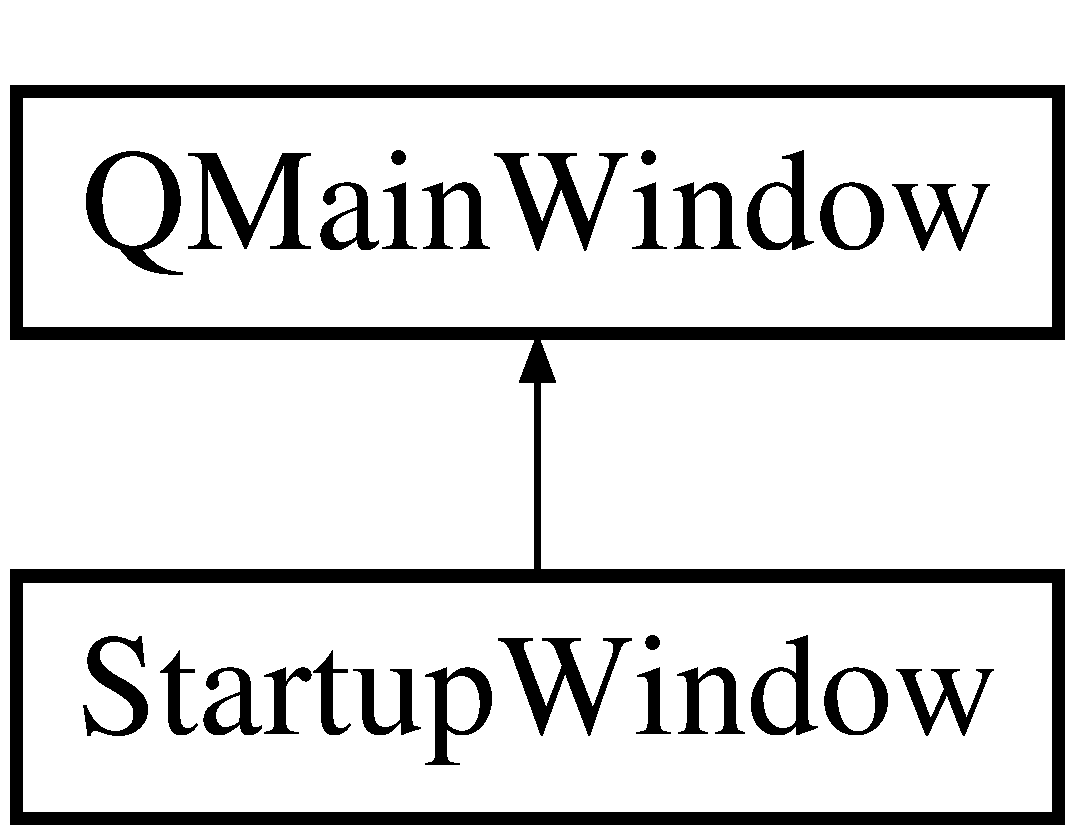
\includegraphics[height=2.000000cm]{dd/d7e/class_startup_window}
\end{center}
\end{figure}
\subsection*{Public Member Functions}
\begin{DoxyCompactItemize}
\item 
\mbox{\hyperlink{class_startup_window_a5aac41515d35e1306d8ac0890f3de174}{Startup\+Window}} (Q\+Widget $\ast$parent=0)
\begin{DoxyCompactList}\small\item\em Constructor for the \mbox{\hyperlink{class_startup_window}{Startup\+Window}}. \end{DoxyCompactList}\item 
\mbox{\hyperlink{class_startup_window_a770398264202b2b44cf188c6a7b919fd}{$\sim$\+Startup\+Window}} ()
\begin{DoxyCompactList}\small\item\em Destructor for the startup window. \end{DoxyCompactList}\end{DoxyCompactItemize}
\subsection*{Private Slots}
\begin{DoxyCompactItemize}
\item 
void \mbox{\hyperlink{class_startup_window_a8b611329fddb960c3c27c54f7d5bf060}{on\+\_\+add\+Folder\+Button\+\_\+released}} ()
\begin{DoxyCompactList}\small\item\em Handles when the Add Folder button is pressed and released. \end{DoxyCompactList}\item 
void \mbox{\hyperlink{class_startup_window_ad0bffaf12ad4255396ccbd709c85922f}{on\+\_\+begin\+Sorting\+Button\+\_\+released}} ()
\begin{DoxyCompactList}\small\item\em Handles the Begin Sorting! button being clicked and released. \end{DoxyCompactList}\item 
void \mbox{\hyperlink{class_startup_window_ac4235050012186e44fbc4e3e3c990d81}{on\+\_\+imported\+Songs\+Confirmed}} ()
\begin{DoxyCompactList}\small\item\em Slot that handles songs being imported. \end{DoxyCompactList}\item 
void \mbox{\hyperlink{class_startup_window_a049e5d9f548d809e89f546d29def2707}{on\+\_\+\+Song\+List\+Viewer\+Window\+Cancelled}} ()
\begin{DoxyCompactList}\small\item\em Slot that handles the \mbox{\hyperlink{class_song_list_viewer_window}{Song\+List\+Viewer\+Window}} being cancelled or exited. \end{DoxyCompactList}\item 
void \mbox{\hyperlink{class_startup_window_a18e7e279255ae11a1121f880d597dae9}{on\+\_\+song\+List\+Edited}} ()
\begin{DoxyCompactList}\small\item\em A slot that handles when the song list is edited in the \mbox{\hyperlink{class_song_list_viewer_window}{Song\+List\+Viewer\+Window}}. \end{DoxyCompactList}\item 
void \mbox{\hyperlink{class_startup_window_afb42686ecfc3556f38889ca53b4d458e}{on\+\_\+view\+Song\+List\+Button\+\_\+released}} ()
\begin{DoxyCompactList}\small\item\em Handles the View Songs button being clicked and released. \end{DoxyCompactList}\end{DoxyCompactItemize}
\subsection*{Private Member Functions}
\begin{DoxyCompactItemize}
\item 
void \mbox{\hyperlink{class_startup_window_adb01cfe36f641352bc2c24a7df6faebd}{parse\+Next\+Song}} ()
\item 
void \mbox{\hyperlink{class_startup_window_adc6941b3def8ed33a8925bef6ad82449}{show\+Song\+List\+Viewer\+Window}} (\mbox{\hyperlink{class_song_list_viewer_window_a6f23a68c416173f6b571a2cc4990a927}{Song\+List\+Viewer\+Window\+::\+S\+O\+N\+G\+\_\+\+L\+I\+S\+T\+\_\+\+M\+O\+DE}} a\+Song\+List\+Mode)
\begin{DoxyCompactList}\small\item\em Shows the \mbox{\hyperlink{class_song_list_viewer_window}{Song\+List\+Viewer\+Window}}. \end{DoxyCompactList}\item 
void \mbox{\hyperlink{class_startup_window_a910d56e4b640d6b7b27a6de2ae18d736}{update\+Ui}} ()
\begin{DoxyCompactList}\small\item\em Updates the the ui based on the state of the main song list. \end{DoxyCompactList}\end{DoxyCompactItemize}
\subsection*{Private Attributes}
\begin{DoxyCompactItemize}
\item 
Ui\+::\+Startup\+Window $\ast$ \mbox{\hyperlink{class_startup_window_a5afeeaabe9a34a02a67d2e7d9f36dc09}{ui}}
\item 
\mbox{\hyperlink{class_comparison_window}{Comparison\+Window}} $\ast$ \mbox{\hyperlink{class_startup_window_a674395b4edbe76568be4f0f4c7577ac1}{m\+Comparison\+Window}} = nullptr
\begin{DoxyCompactList}\small\item\em The window for comparing pairs of songs. \end{DoxyCompactList}\item 
\mbox{\hyperlink{class_song_list_viewer_window}{Song\+List\+Viewer\+Window}} $\ast$ \mbox{\hyperlink{class_startup_window_a26e72433e3cf3d35ae49d77d91f5cc38}{m\+Song\+List\+Viewer\+Window}} = nullptr
\begin{DoxyCompactList}\small\item\em The window for viewing lists of songs. \end{DoxyCompactList}\item 
Q\+List$<$ \mbox{\hyperlink{class_song}{Song}} $\ast$ $>$ \mbox{\hyperlink{class_startup_window_ae57241505d74639131cb0ece2cfc922b}{m\+Songs}}
\begin{DoxyCompactList}\small\item\em The main song list. \end{DoxyCompactList}\item 
Q\+List$<$ \mbox{\hyperlink{class_song}{Song}} $\ast$ $>$ \mbox{\hyperlink{class_startup_window_af419f4809f6fae0b370f1d9112dae9b4}{m\+Songs\+From\+Selected\+Folder}}
\begin{DoxyCompactList}\small\item\em A temporary list of songs from an imported folder. \end{DoxyCompactList}\end{DoxyCompactItemize}
\subsection*{Static Private Attributes}
\begin{DoxyCompactItemize}
\item 
static const Q\+String \mbox{\hyperlink{class_startup_window_a59337faf9ce34917d0e056414601c571}{m\+Num\+Songs\+Label}} = Q\+String(\char`\"{}Number of songs that will be sorted\+: \char`\"{})
\begin{DoxyCompactList}\small\item\em A label for the number of songs in the main song list. \end{DoxyCompactList}\item 
static Q\+String\+List \mbox{\hyperlink{class_startup_window_a7caf611224e692a7116cba45f1aa71a3}{ms\+Supported\+File\+Extensions}} = Q\+String\+List() $<$$<$ \char`\"{}$\ast$.mp3\char`\"{} $<$$<$ \char`\"{}$\ast$.flac\char`\"{}
\begin{DoxyCompactList}\small\item\em The file extensions that are searched for in a selected folder. \end{DoxyCompactList}\end{DoxyCompactItemize}


\subsection{Detailed Description}
Contains the UI handling for the startup window.

The startup window is pretty much the main window of the program. It allows for users to import songs, edit imported songs, and begin sorting once songs are imported. 

Definition at line 21 of file startupwindow.\+h.



\subsection{Constructor \& Destructor Documentation}
\mbox{\Hypertarget{class_startup_window_a5aac41515d35e1306d8ac0890f3de174}\label{class_startup_window_a5aac41515d35e1306d8ac0890f3de174}} 
\index{Startup\+Window@{Startup\+Window}!Startup\+Window@{Startup\+Window}}
\index{Startup\+Window@{Startup\+Window}!Startup\+Window@{Startup\+Window}}
\subsubsection{\texorpdfstring{Startup\+Window()}{StartupWindow()}}
{\footnotesize\ttfamily Startup\+Window\+::\+Startup\+Window (\begin{DoxyParamCaption}\item[{Q\+Widget $\ast$}]{parent = {\ttfamily 0} }\end{DoxyParamCaption})\hspace{0.3cm}{\ttfamily [explicit]}}



Constructor for the \mbox{\hyperlink{class_startup_window}{Startup\+Window}}. 


\begin{DoxyParams}{Parameters}
{\em parent} & The parent of the window.\\
\hline
\end{DoxyParams}
The constructor sets up the UI for the \mbox{\hyperlink{class_startup_window}{Startup\+Window}} and connects signals to its slots. 

Definition at line 33 of file startupwindow.\+cpp.


\begin{DoxyCode}
33                                             :
34     QMainWindow(parent),
35     \mbox{\hyperlink{class_startup_window_a5afeeaabe9a34a02a67d2e7d9f36dc09}{ui}}(\textcolor{keyword}{new} Ui::StartupWindow)
36 \{
37     \textcolor{comment}{// Set up the UI and other windows.}
38     \mbox{\hyperlink{class_startup_window_a5afeeaabe9a34a02a67d2e7d9f36dc09}{ui}}->setupUi(\textcolor{keyword}{this});
39     \mbox{\hyperlink{class_startup_window_a674395b4edbe76568be4f0f4c7577ac1}{mComparisonWindow}} = \textcolor{keyword}{new} \mbox{\hyperlink{class_comparison_window}{ComparisonWindow}}(\textcolor{keyword}{this});
40     \mbox{\hyperlink{class_startup_window_a26e72433e3cf3d35ae49d77d91f5cc38}{mSongListViewerWindow}} = \textcolor{keyword}{new} \mbox{\hyperlink{class_song_list_viewer_window}{SongListViewerWindow}}(\textcolor{keyword}{this});
41     \mbox{\hyperlink{class_startup_window_a674395b4edbe76568be4f0f4c7577ac1}{mComparisonWindow}}->hide();
42     \mbox{\hyperlink{class_startup_window_a26e72433e3cf3d35ae49d77d91f5cc38}{mSongListViewerWindow}}->hide();
43     \mbox{\hyperlink{class_startup_window_a5afeeaabe9a34a02a67d2e7d9f36dc09}{ui}}->viewSongListButton->setEnabled(\textcolor{keyword}{false});
44     \mbox{\hyperlink{class_startup_window_a5afeeaabe9a34a02a67d2e7d9f36dc09}{ui}}->beginSortingButton->setEnabled(\textcolor{keyword}{false});
45 
46     \textcolor{comment}{// Connect slots.}
47     connect(\mbox{\hyperlink{class_startup_window_a26e72433e3cf3d35ae49d77d91f5cc38}{mSongListViewerWindow}}, SIGNAL(importedSongsConfirmed()), \textcolor{keyword}{this}, SLOT(
      \mbox{\hyperlink{class_startup_window_ac4235050012186e44fbc4e3e3c990d81}{on\_importedSongsConfirmed}}()));
48     connect(\mbox{\hyperlink{class_startup_window_a26e72433e3cf3d35ae49d77d91f5cc38}{mSongListViewerWindow}}, SIGNAL(songListEdited()), \textcolor{keyword}{this}, SLOT(
      \mbox{\hyperlink{class_startup_window_a18e7e279255ae11a1121f880d597dae9}{on\_songListEdited}}()));
49     connect(\mbox{\hyperlink{class_startup_window_a26e72433e3cf3d35ae49d77d91f5cc38}{mSongListViewerWindow}}, SIGNAL(importCancelled()), \textcolor{keyword}{this}, SLOT(
      \mbox{\hyperlink{class_startup_window_a049e5d9f548d809e89f546d29def2707}{on\_SongListViewerWindowCancelled}}()));
50 \}
\end{DoxyCode}
\mbox{\Hypertarget{class_startup_window_a770398264202b2b44cf188c6a7b919fd}\label{class_startup_window_a770398264202b2b44cf188c6a7b919fd}} 
\index{Startup\+Window@{Startup\+Window}!````~Startup\+Window@{$\sim$\+Startup\+Window}}
\index{````~Startup\+Window@{$\sim$\+Startup\+Window}!Startup\+Window@{Startup\+Window}}
\subsubsection{\texorpdfstring{$\sim$\+Startup\+Window()}{~StartupWindow()}}
{\footnotesize\ttfamily Startup\+Window\+::$\sim$\+Startup\+Window (\begin{DoxyParamCaption}{ }\end{DoxyParamCaption})}



Destructor for the startup window. 



Definition at line 55 of file startupwindow.\+cpp.


\begin{DoxyCode}
56 \{
57     \textcolor{keyword}{delete} \mbox{\hyperlink{class_startup_window_a5afeeaabe9a34a02a67d2e7d9f36dc09}{ui}};
58 
59     \textcolor{comment}{// Delete the songs in the main list.}
60     \mbox{\hyperlink{class_song}{Song}}* songToDelete = \textcolor{keyword}{nullptr};
61     QMutableListIterator<Song*> iter(\mbox{\hyperlink{class_startup_window_ae57241505d74639131cb0ece2cfc922b}{mSongs}});
62     \textcolor{keywordflow}{while}(iter.hasNext())
63     \{
64         songToDelete = iter.next();
65         iter.remove();
66         \textcolor{keyword}{delete} songToDelete;
67         songToDelete = \textcolor{keyword}{nullptr};
68     \}
69 
70     \textcolor{comment}{// Delete the songs in the imported song list.}
71     iter = QMutableListIterator<Song*>(\mbox{\hyperlink{class_startup_window_af419f4809f6fae0b370f1d9112dae9b4}{mSongsFromSelectedFolder}});
72     \textcolor{keywordflow}{while}(iter.hasNext())
73     \{
74         songToDelete = iter.next();
75         iter.remove();
76         \textcolor{keyword}{delete} songToDelete;
77         songToDelete = \textcolor{keyword}{nullptr};
78     \}
79 
80 \}
\end{DoxyCode}


\subsection{Member Function Documentation}
\mbox{\Hypertarget{class_startup_window_a8b611329fddb960c3c27c54f7d5bf060}\label{class_startup_window_a8b611329fddb960c3c27c54f7d5bf060}} 
\index{Startup\+Window@{Startup\+Window}!on\+\_\+add\+Folder\+Button\+\_\+released@{on\+\_\+add\+Folder\+Button\+\_\+released}}
\index{on\+\_\+add\+Folder\+Button\+\_\+released@{on\+\_\+add\+Folder\+Button\+\_\+released}!Startup\+Window@{Startup\+Window}}
\subsubsection{\texorpdfstring{on\+\_\+add\+Folder\+Button\+\_\+released}{on\_addFolderButton\_released}}
{\footnotesize\ttfamily void Startup\+Window\+::on\+\_\+add\+Folder\+Button\+\_\+released (\begin{DoxyParamCaption}{ }\end{DoxyParamCaption})\hspace{0.3cm}{\ttfamily [private]}, {\ttfamily [slot]}}



Handles when the Add Folder button is pressed and released. 

When the Add Folder button is pressed and released, a dialog will show to allow the user to pick a folder of songs that will be added to the list of songs to sort. 

Definition at line 93 of file startupwindow.\+cpp.


\begin{DoxyCode}
94 \{
95     \textcolor{comment}{// Show the open folder dialog and get the chosen directory.}
96     QFileDialog openFolderDialog;
97     openFolderDialog.setFileMode(QFileDialog::DirectoryOnly);
98     QString openedDirectory = openFolderDialog.getExistingDirectory();
99 
100     \textcolor{keywordflow}{if}(openedDirectory != \textcolor{stringliteral}{""})
101     \{
102         \textcolor{comment}{// If the chosen directory contains songs to import, then get their metadata and create a container
       for them.}
103         QDirIterator iter(openedDirectory, \mbox{\hyperlink{class_startup_window_a7caf611224e692a7116cba45f1aa71a3}{msSupportedFileExtensions}}, 
      QDir::Filter::NoFilter, QDirIterator::FollowSymlinks|QDirIterator::Subdirectories);
104         \textcolor{keywordflow}{if}(iter.hasNext())
105         \{
106             \textcolor{comment}{// Declare variables.}
107             TagLib::FileRef file;
108             \textcolor{keywordtype}{int} currentPathLength = 0;
109             \textcolor{keywordtype}{int} trackNumber = 1;
110             QString currentPath, artist, album, songName;
111             \mbox{\hyperlink{class_song}{Song}}* newSong = \textcolor{keyword}{nullptr};
112             \textcolor{keywordtype}{wchar\_t}* filePathForTaglib = \textcolor{keyword}{nullptr};
113 
114             \textcolor{comment}{// Get the metadata of all of the songs in the chosen directory.}
115             \textcolor{keywordflow}{while}(iter.hasNext())
116             \{
117                 \textcolor{comment}{// Convert the QString containing the current path so that we can use it with taglib.}
118                 currentPath = iter.next();
119                 currentPathLength = currentPath.length();
120                 filePathForTaglib = \textcolor{keyword}{new} \textcolor{keywordtype}{wchar\_t}[currentPathLength + 1];
121                 currentPath.toWCharArray(filePathForTaglib);
122                 filePathForTaglib[currentPathLength] = L\textcolor{charliteral}{'\(\backslash\)0'};
123 
124                 \textcolor{comment}{// Use Taglib to get the metadata of the song.}
125                 file = TagLib::FileRef(TagLib::FileName(filePathForTaglib));
126                 \textcolor{keywordflow}{if}(!file.isNull() && file.tag() != \textcolor{keyword}{nullptr})
127                 \{
128                     artist = QString(file.tag()->artist().toCString(\textcolor{keyword}{true}));
129                     album = QString(file.tag()->album().toCString(\textcolor{keyword}{true}));
130                     songName = QString(file.tag()->title().toCString(\textcolor{keyword}{true}));
131                     trackNumber = (int)file.tag()->track();
132                     newSong = \textcolor{keyword}{new} \mbox{\hyperlink{class_song}{Song}}(trackNumber, album, artist, currentPath, songName);
133 
134                     \textcolor{comment}{// Add the new song to the list of imported songs.}
135                     \mbox{\hyperlink{class_startup_window_af419f4809f6fae0b370f1d9112dae9b4}{mSongsFromSelectedFolder}}.append(newSong);
136                 \}
137 
138                 \textcolor{comment}{// Clear allocated memory.}
139                 \textcolor{keyword}{delete} [] filePathForTaglib;
140                 filePathForTaglib = \textcolor{keyword}{nullptr};
141             \}
142         \}
143     \}
144 
145     \textcolor{comment}{// If we found songs in the selected folder, then let the user confirm which ones they want to import.}
146     \textcolor{keywordflow}{if}(\mbox{\hyperlink{class_startup_window_af419f4809f6fae0b370f1d9112dae9b4}{mSongsFromSelectedFolder}}.count() > 0)
147     \{
148         \mbox{\hyperlink{class_startup_window_adc6941b3def8ed33a8925bef6ad82449}{showSongListViewerWindow}}(
      SongListViewerWindow::SONG\_LIST\_MODE::CONFIRM\_IMPORTED\_SONGS);
149     \}
150 \}
\end{DoxyCode}
\mbox{\Hypertarget{class_startup_window_ad0bffaf12ad4255396ccbd709c85922f}\label{class_startup_window_ad0bffaf12ad4255396ccbd709c85922f}} 
\index{Startup\+Window@{Startup\+Window}!on\+\_\+begin\+Sorting\+Button\+\_\+released@{on\+\_\+begin\+Sorting\+Button\+\_\+released}}
\index{on\+\_\+begin\+Sorting\+Button\+\_\+released@{on\+\_\+begin\+Sorting\+Button\+\_\+released}!Startup\+Window@{Startup\+Window}}
\subsubsection{\texorpdfstring{on\+\_\+begin\+Sorting\+Button\+\_\+released}{on\_beginSortingButton\_released}}
{\footnotesize\ttfamily void Startup\+Window\+::on\+\_\+begin\+Sorting\+Button\+\_\+released (\begin{DoxyParamCaption}{ }\end{DoxyParamCaption})\hspace{0.3cm}{\ttfamily [private]}, {\ttfamily [slot]}}



Handles the Begin Sorting! button being clicked and released. 

This function will close the \mbox{\hyperlink{class_startup_window}{Startup\+Window}} and open the \mbox{\hyperlink{class_comparison_window}{Comparison\+Window}} to begin sorting the songs. 

Definition at line 158 of file startupwindow.\+cpp.


\begin{DoxyCode}
159 \{
160     \mbox{\hyperlink{class_startup_window_a674395b4edbe76568be4f0f4c7577ac1}{mComparisonWindow}}->show();
161     hide();
162 \}
\end{DoxyCode}
\mbox{\Hypertarget{class_startup_window_ac4235050012186e44fbc4e3e3c990d81}\label{class_startup_window_ac4235050012186e44fbc4e3e3c990d81}} 
\index{Startup\+Window@{Startup\+Window}!on\+\_\+imported\+Songs\+Confirmed@{on\+\_\+imported\+Songs\+Confirmed}}
\index{on\+\_\+imported\+Songs\+Confirmed@{on\+\_\+imported\+Songs\+Confirmed}!Startup\+Window@{Startup\+Window}}
\subsubsection{\texorpdfstring{on\+\_\+imported\+Songs\+Confirmed}{on\_importedSongsConfirmed}}
{\footnotesize\ttfamily void Startup\+Window\+::on\+\_\+imported\+Songs\+Confirmed (\begin{DoxyParamCaption}{ }\end{DoxyParamCaption})\hspace{0.3cm}{\ttfamily [private]}, {\ttfamily [slot]}}



Slot that handles songs being imported. 

This slot will be called when the \mbox{\hyperlink{class_song_list_viewer_window}{Song\+List\+Viewer\+Window}} is accepted and its \mbox{\hyperlink{class_song_list_viewer_window_a6f23a68c416173f6b571a2cc4990a927}{mode}} is set to C\+O\+N\+F\+I\+R\+M\+\_\+\+I\+M\+P\+O\+R\+T\+E\+D\+\_\+\+S\+O\+N\+GS. 

Definition at line 171 of file startupwindow.\+cpp.


\begin{DoxyCode}
172 \{
173     \textcolor{comment}{// Re-enable the "Add a Folder" button.}
174     \mbox{\hyperlink{class_startup_window_a5afeeaabe9a34a02a67d2e7d9f36dc09}{ui}}->addFolderButton->setEnabled(\textcolor{keyword}{true});
175 
176     \textcolor{comment}{// Append the imported songs to the main list.}
177     \mbox{\hyperlink{class_startup_window_ae57241505d74639131cb0ece2cfc922b}{mSongs}}.append(\mbox{\hyperlink{class_startup_window_af419f4809f6fae0b370f1d9112dae9b4}{mSongsFromSelectedFolder}});
178     \mbox{\hyperlink{class_startup_window_af419f4809f6fae0b370f1d9112dae9b4}{mSongsFromSelectedFolder}}.clear();
179 
180     \textcolor{comment}{// Update the ui.}
181     show();
182     \mbox{\hyperlink{class_startup_window_a910d56e4b640d6b7b27a6de2ae18d736}{updateUi}}();
183 \}
\end{DoxyCode}
\mbox{\Hypertarget{class_startup_window_a18e7e279255ae11a1121f880d597dae9}\label{class_startup_window_a18e7e279255ae11a1121f880d597dae9}} 
\index{Startup\+Window@{Startup\+Window}!on\+\_\+song\+List\+Edited@{on\+\_\+song\+List\+Edited}}
\index{on\+\_\+song\+List\+Edited@{on\+\_\+song\+List\+Edited}!Startup\+Window@{Startup\+Window}}
\subsubsection{\texorpdfstring{on\+\_\+song\+List\+Edited}{on\_songListEdited}}
{\footnotesize\ttfamily void Startup\+Window\+::on\+\_\+song\+List\+Edited (\begin{DoxyParamCaption}{ }\end{DoxyParamCaption})\hspace{0.3cm}{\ttfamily [private]}, {\ttfamily [slot]}}



A slot that handles when the song list is edited in the \mbox{\hyperlink{class_song_list_viewer_window}{Song\+List\+Viewer\+Window}}. 

This function checks if there are still songs in the \mbox{\hyperlink{class_startup_window_ae57241505d74639131cb0ece2cfc922b}{main song list}} and updates the UI accordingly. 

Definition at line 191 of file startupwindow.\+cpp.


\begin{DoxyCode}
192 \{
193     show();
194     \mbox{\hyperlink{class_startup_window_a5afeeaabe9a34a02a67d2e7d9f36dc09}{ui}}->addFolderButton->setEnabled(\textcolor{keyword}{true});
195     \mbox{\hyperlink{class_startup_window_a910d56e4b640d6b7b27a6de2ae18d736}{updateUi}}();
196 \}
\end{DoxyCode}
\mbox{\Hypertarget{class_startup_window_a049e5d9f548d809e89f546d29def2707}\label{class_startup_window_a049e5d9f548d809e89f546d29def2707}} 
\index{Startup\+Window@{Startup\+Window}!on\+\_\+\+Song\+List\+Viewer\+Window\+Cancelled@{on\+\_\+\+Song\+List\+Viewer\+Window\+Cancelled}}
\index{on\+\_\+\+Song\+List\+Viewer\+Window\+Cancelled@{on\+\_\+\+Song\+List\+Viewer\+Window\+Cancelled}!Startup\+Window@{Startup\+Window}}
\subsubsection{\texorpdfstring{on\+\_\+\+Song\+List\+Viewer\+Window\+Cancelled}{on\_SongListViewerWindowCancelled}}
{\footnotesize\ttfamily void Startup\+Window\+::on\+\_\+\+Song\+List\+Viewer\+Window\+Cancelled (\begin{DoxyParamCaption}{ }\end{DoxyParamCaption})\hspace{0.3cm}{\ttfamily [private]}, {\ttfamily [slot]}}



Slot that handles the \mbox{\hyperlink{class_song_list_viewer_window}{Song\+List\+Viewer\+Window}} being cancelled or exited. 

This function just resets the import process and updates the ui. 

Definition at line 203 of file startupwindow.\+cpp.


\begin{DoxyCode}
204 \{
205     \mbox{\hyperlink{class_startup_window_a5afeeaabe9a34a02a67d2e7d9f36dc09}{ui}}->addFolderButton->setEnabled(\textcolor{keyword}{true});
206     \mbox{\hyperlink{class_startup_window_af419f4809f6fae0b370f1d9112dae9b4}{mSongsFromSelectedFolder}}.clear();
207     show();
208     \mbox{\hyperlink{class_startup_window_a910d56e4b640d6b7b27a6de2ae18d736}{updateUi}}();
209 \}
\end{DoxyCode}
\mbox{\Hypertarget{class_startup_window_afb42686ecfc3556f38889ca53b4d458e}\label{class_startup_window_afb42686ecfc3556f38889ca53b4d458e}} 
\index{Startup\+Window@{Startup\+Window}!on\+\_\+view\+Song\+List\+Button\+\_\+released@{on\+\_\+view\+Song\+List\+Button\+\_\+released}}
\index{on\+\_\+view\+Song\+List\+Button\+\_\+released@{on\+\_\+view\+Song\+List\+Button\+\_\+released}!Startup\+Window@{Startup\+Window}}
\subsubsection{\texorpdfstring{on\+\_\+view\+Song\+List\+Button\+\_\+released}{on\_viewSongListButton\_released}}
{\footnotesize\ttfamily void Startup\+Window\+::on\+\_\+view\+Song\+List\+Button\+\_\+released (\begin{DoxyParamCaption}{ }\end{DoxyParamCaption})\hspace{0.3cm}{\ttfamily [private]}, {\ttfamily [slot]}}



Handles the View Songs button being clicked and released. 

This function will show the \mbox{\hyperlink{class_song_list_viewer_window}{Song\+List\+Viewer\+Window}} and populate it with \mbox{\hyperlink{class_startup_window_af419f4809f6fae0b370f1d9112dae9b4}{the current imported songs}}. 

Definition at line 217 of file startupwindow.\+cpp.


\begin{DoxyCode}
218 \{
219     \mbox{\hyperlink{class_startup_window_adc6941b3def8ed33a8925bef6ad82449}{showSongListViewerWindow}}(
      SongListViewerWindow::SONG\_LIST\_MODE::EDIT\_MAIN\_SONG\_LIST);
220 \}
\end{DoxyCode}
\mbox{\Hypertarget{class_startup_window_adb01cfe36f641352bc2c24a7df6faebd}\label{class_startup_window_adb01cfe36f641352bc2c24a7df6faebd}} 
\index{Startup\+Window@{Startup\+Window}!parse\+Next\+Song@{parse\+Next\+Song}}
\index{parse\+Next\+Song@{parse\+Next\+Song}!Startup\+Window@{Startup\+Window}}
\subsubsection{\texorpdfstring{parse\+Next\+Song()}{parseNextSong()}}
{\footnotesize\ttfamily void Startup\+Window\+::parse\+Next\+Song (\begin{DoxyParamCaption}{ }\end{DoxyParamCaption})\hspace{0.3cm}{\ttfamily [private]}}

\mbox{\Hypertarget{class_startup_window_adc6941b3def8ed33a8925bef6ad82449}\label{class_startup_window_adc6941b3def8ed33a8925bef6ad82449}} 
\index{Startup\+Window@{Startup\+Window}!show\+Song\+List\+Viewer\+Window@{show\+Song\+List\+Viewer\+Window}}
\index{show\+Song\+List\+Viewer\+Window@{show\+Song\+List\+Viewer\+Window}!Startup\+Window@{Startup\+Window}}
\subsubsection{\texorpdfstring{show\+Song\+List\+Viewer\+Window()}{showSongListViewerWindow()}}
{\footnotesize\ttfamily void Startup\+Window\+::show\+Song\+List\+Viewer\+Window (\begin{DoxyParamCaption}\item[{\mbox{\hyperlink{class_song_list_viewer_window_a6f23a68c416173f6b571a2cc4990a927}{Song\+List\+Viewer\+Window\+::\+S\+O\+N\+G\+\_\+\+L\+I\+S\+T\+\_\+\+M\+O\+DE}}}]{a\+Song\+List\+Mode }\end{DoxyParamCaption})\hspace{0.3cm}{\ttfamily [private]}}



Shows the \mbox{\hyperlink{class_song_list_viewer_window}{Song\+List\+Viewer\+Window}}. 


\begin{DoxyParams}{Parameters}
{\em a\+Song\+List\+Mode} & The \mbox{\hyperlink{class_song_list_viewer_window_a6f23a68c416173f6b571a2cc4990a927}{mode}} in which to run the song list viewer. \\
\hline
\end{DoxyParams}


Definition at line 230 of file startupwindow.\+cpp.


\begin{DoxyCode}
231 \{
232     \textcolor{comment}{// Update the ui since we're showing the dialog.}
233     \mbox{\hyperlink{class_startup_window_a5afeeaabe9a34a02a67d2e7d9f36dc09}{ui}}->addFolderButton->setEnabled(\textcolor{keyword}{false});
234 
235     \textcolor{comment}{// Setup the window and show it.}
236     \textcolor{keywordflow}{if}(aSongListMode == SongListViewerWindow::SONG\_LIST\_MODE::CONFIRM\_IMPORTED\_SONGS)
237     \{
238         \mbox{\hyperlink{class_startup_window_a26e72433e3cf3d35ae49d77d91f5cc38}{mSongListViewerWindow}}->\mbox{\hyperlink{class_song_list_viewer_window_ae26127c85ed57885461c5143be4ae1e9}{setupSongListViewerWindow}}(
      aSongListMode, &\mbox{\hyperlink{class_startup_window_af419f4809f6fae0b370f1d9112dae9b4}{mSongsFromSelectedFolder}});
239     \}
240     \textcolor{keywordflow}{else}
241     \{
242         \mbox{\hyperlink{class_startup_window_a26e72433e3cf3d35ae49d77d91f5cc38}{mSongListViewerWindow}}->\mbox{\hyperlink{class_song_list_viewer_window_ae26127c85ed57885461c5143be4ae1e9}{setupSongListViewerWindow}}(
      aSongListMode, &\mbox{\hyperlink{class_startup_window_ae57241505d74639131cb0ece2cfc922b}{mSongs}});
243     \}
244     \mbox{\hyperlink{class_startup_window_a26e72433e3cf3d35ae49d77d91f5cc38}{mSongListViewerWindow}}->show();
245     hide();
246 \}
\end{DoxyCode}
\mbox{\Hypertarget{class_startup_window_a910d56e4b640d6b7b27a6de2ae18d736}\label{class_startup_window_a910d56e4b640d6b7b27a6de2ae18d736}} 
\index{Startup\+Window@{Startup\+Window}!update\+Ui@{update\+Ui}}
\index{update\+Ui@{update\+Ui}!Startup\+Window@{Startup\+Window}}
\subsubsection{\texorpdfstring{update\+Ui()}{updateUi()}}
{\footnotesize\ttfamily void Startup\+Window\+::update\+Ui (\begin{DoxyParamCaption}{ }\end{DoxyParamCaption})\hspace{0.3cm}{\ttfamily [private]}}



Updates the the ui based on the state of the main song list. 



Definition at line 251 of file startupwindow.\+cpp.


\begin{DoxyCode}
252 \{
253     \textcolor{keywordtype}{bool} enableViewAndSortButtons = !\mbox{\hyperlink{class_startup_window_ae57241505d74639131cb0ece2cfc922b}{mSongs}}.empty();
254     \mbox{\hyperlink{class_startup_window_a5afeeaabe9a34a02a67d2e7d9f36dc09}{ui}}->beginSortingButton->setEnabled(enableViewAndSortButtons);
255     \mbox{\hyperlink{class_startup_window_a5afeeaabe9a34a02a67d2e7d9f36dc09}{ui}}->viewSongListButton->setEnabled(enableViewAndSortButtons);
256     \textcolor{keywordflow}{if}(\mbox{\hyperlink{class_startup_window_ae57241505d74639131cb0ece2cfc922b}{mSongs}}.count() > 0)
257     \{
258         \mbox{\hyperlink{class_startup_window_a5afeeaabe9a34a02a67d2e7d9f36dc09}{ui}}->numSongsLabel->show();
259         \mbox{\hyperlink{class_startup_window_a5afeeaabe9a34a02a67d2e7d9f36dc09}{ui}}->numSongsLabel->setText(\mbox{\hyperlink{class_startup_window_a59337faf9ce34917d0e056414601c571}{StartupWindow::mNumSongsLabel}} + QString(\textcolor{stringliteral}{"
      %1"}).arg(\mbox{\hyperlink{class_startup_window_ae57241505d74639131cb0ece2cfc922b}{mSongs}}.count()));
260     \}
261     \textcolor{keywordflow}{else}
262     \{
263         \mbox{\hyperlink{class_startup_window_a5afeeaabe9a34a02a67d2e7d9f36dc09}{ui}}->numSongsLabel->hide();
264     \}
265 \}
\end{DoxyCode}


\subsection{Member Data Documentation}
\mbox{\Hypertarget{class_startup_window_a674395b4edbe76568be4f0f4c7577ac1}\label{class_startup_window_a674395b4edbe76568be4f0f4c7577ac1}} 
\index{Startup\+Window@{Startup\+Window}!m\+Comparison\+Window@{m\+Comparison\+Window}}
\index{m\+Comparison\+Window@{m\+Comparison\+Window}!Startup\+Window@{Startup\+Window}}
\subsubsection{\texorpdfstring{m\+Comparison\+Window}{mComparisonWindow}}
{\footnotesize\ttfamily \mbox{\hyperlink{class_comparison_window}{Comparison\+Window}}$\ast$ Startup\+Window\+::m\+Comparison\+Window = nullptr\hspace{0.3cm}{\ttfamily [private]}}



The window for comparing pairs of songs. 



Definition at line 44 of file startupwindow.\+h.

\mbox{\Hypertarget{class_startup_window_a59337faf9ce34917d0e056414601c571}\label{class_startup_window_a59337faf9ce34917d0e056414601c571}} 
\index{Startup\+Window@{Startup\+Window}!m\+Num\+Songs\+Label@{m\+Num\+Songs\+Label}}
\index{m\+Num\+Songs\+Label@{m\+Num\+Songs\+Label}!Startup\+Window@{Startup\+Window}}
\subsubsection{\texorpdfstring{m\+Num\+Songs\+Label}{mNumSongsLabel}}
{\footnotesize\ttfamily const Q\+String Startup\+Window\+::m\+Num\+Songs\+Label = Q\+String(\char`\"{}Number of songs that will be sorted\+: \char`\"{})\hspace{0.3cm}{\ttfamily [static]}, {\ttfamily [private]}}



A label for the number of songs in the main song list. 



Definition at line 49 of file startupwindow.\+h.

\mbox{\Hypertarget{class_startup_window_a26e72433e3cf3d35ae49d77d91f5cc38}\label{class_startup_window_a26e72433e3cf3d35ae49d77d91f5cc38}} 
\index{Startup\+Window@{Startup\+Window}!m\+Song\+List\+Viewer\+Window@{m\+Song\+List\+Viewer\+Window}}
\index{m\+Song\+List\+Viewer\+Window@{m\+Song\+List\+Viewer\+Window}!Startup\+Window@{Startup\+Window}}
\subsubsection{\texorpdfstring{m\+Song\+List\+Viewer\+Window}{mSongListViewerWindow}}
{\footnotesize\ttfamily \mbox{\hyperlink{class_song_list_viewer_window}{Song\+List\+Viewer\+Window}}$\ast$ Startup\+Window\+::m\+Song\+List\+Viewer\+Window = nullptr\hspace{0.3cm}{\ttfamily [private]}}



The window for viewing lists of songs. 



Definition at line 45 of file startupwindow.\+h.

\mbox{\Hypertarget{class_startup_window_ae57241505d74639131cb0ece2cfc922b}\label{class_startup_window_ae57241505d74639131cb0ece2cfc922b}} 
\index{Startup\+Window@{Startup\+Window}!m\+Songs@{m\+Songs}}
\index{m\+Songs@{m\+Songs}!Startup\+Window@{Startup\+Window}}
\subsubsection{\texorpdfstring{m\+Songs}{mSongs}}
{\footnotesize\ttfamily Q\+List$<$\mbox{\hyperlink{class_song}{Song}}$\ast$$>$ Startup\+Window\+::m\+Songs\hspace{0.3cm}{\ttfamily [private]}}



The main song list. 



Definition at line 46 of file startupwindow.\+h.

\mbox{\Hypertarget{class_startup_window_af419f4809f6fae0b370f1d9112dae9b4}\label{class_startup_window_af419f4809f6fae0b370f1d9112dae9b4}} 
\index{Startup\+Window@{Startup\+Window}!m\+Songs\+From\+Selected\+Folder@{m\+Songs\+From\+Selected\+Folder}}
\index{m\+Songs\+From\+Selected\+Folder@{m\+Songs\+From\+Selected\+Folder}!Startup\+Window@{Startup\+Window}}
\subsubsection{\texorpdfstring{m\+Songs\+From\+Selected\+Folder}{mSongsFromSelectedFolder}}
{\footnotesize\ttfamily Q\+List$<$\mbox{\hyperlink{class_song}{Song}}$\ast$$>$ Startup\+Window\+::m\+Songs\+From\+Selected\+Folder\hspace{0.3cm}{\ttfamily [private]}}



A temporary list of songs from an imported folder. 



Definition at line 47 of file startupwindow.\+h.

\mbox{\Hypertarget{class_startup_window_a7caf611224e692a7116cba45f1aa71a3}\label{class_startup_window_a7caf611224e692a7116cba45f1aa71a3}} 
\index{Startup\+Window@{Startup\+Window}!ms\+Supported\+File\+Extensions@{ms\+Supported\+File\+Extensions}}
\index{ms\+Supported\+File\+Extensions@{ms\+Supported\+File\+Extensions}!Startup\+Window@{Startup\+Window}}
\subsubsection{\texorpdfstring{ms\+Supported\+File\+Extensions}{msSupportedFileExtensions}}
{\footnotesize\ttfamily Q\+String\+List Startup\+Window\+::ms\+Supported\+File\+Extensions = Q\+String\+List() $<$$<$ \char`\"{}$\ast$.mp3\char`\"{} $<$$<$ \char`\"{}$\ast$.flac\char`\"{}\hspace{0.3cm}{\ttfamily [static]}, {\ttfamily [private]}}



The file extensions that are searched for in a selected folder. 



Definition at line 50 of file startupwindow.\+h.

\mbox{\Hypertarget{class_startup_window_a5afeeaabe9a34a02a67d2e7d9f36dc09}\label{class_startup_window_a5afeeaabe9a34a02a67d2e7d9f36dc09}} 
\index{Startup\+Window@{Startup\+Window}!ui@{ui}}
\index{ui@{ui}!Startup\+Window@{Startup\+Window}}
\subsubsection{\texorpdfstring{ui}{ui}}
{\footnotesize\ttfamily Ui\+::\+Startup\+Window$\ast$ Startup\+Window\+::ui\hspace{0.3cm}{\ttfamily [private]}}



Definition at line 42 of file startupwindow.\+h.



The documentation for this class was generated from the following files\+:\begin{DoxyCompactItemize}
\item 
U\+I/\mbox{\hyperlink{startupwindow_8h}{startupwindow.\+h}}\item 
U\+I/\mbox{\hyperlink{startupwindow_8cpp}{startupwindow.\+cpp}}\end{DoxyCompactItemize}

\chapter{File Documentation}
\hypertarget{documentation_8dox}{}\section{doc/documentation.dox File Reference}
\label{documentation_8dox}\index{doc/documentation.\+dox@{doc/documentation.\+dox}}

\hypertarget{main_8cpp}{}\section{main.\+cpp File Reference}
\label{main_8cpp}\index{main.\+cpp@{main.\+cpp}}
{\ttfamily \#include \char`\"{}U\+I/startupwindow.\+h\char`\"{}}\newline
{\ttfamily \#include $<$Q\+Application$>$}\newline
\subsection*{Functions}
\begin{DoxyCompactItemize}
\item 
int \mbox{\hyperlink{main_8cpp_a0ddf1224851353fc92bfbff6f499fa97}{main}} (int argc, char $\ast$argv\mbox{[}$\,$\mbox{]})
\end{DoxyCompactItemize}


\subsection{Function Documentation}
\mbox{\Hypertarget{main_8cpp_a0ddf1224851353fc92bfbff6f499fa97}\label{main_8cpp_a0ddf1224851353fc92bfbff6f499fa97}} 
\index{main.\+cpp@{main.\+cpp}!main@{main}}
\index{main@{main}!main.\+cpp@{main.\+cpp}}
\subsubsection{\texorpdfstring{main()}{main()}}
{\footnotesize\ttfamily int main (\begin{DoxyParamCaption}\item[{int}]{argc,  }\item[{char $\ast$}]{argv\mbox{[}$\,$\mbox{]} }\end{DoxyParamCaption})}



Definition at line 4 of file main.\+cpp.


\begin{DoxyCode}
5 \{
6     QApplication a(argc, argv);
7     \mbox{\hyperlink{class_startup_window}{StartupWindow}} w;
8     w.show();
9 
10     \textcolor{keywordflow}{return} a.exec();
11 \}
\end{DoxyCode}

\hypertarget{_r_e_a_d_m_e_8md}{}\section{R\+E\+A\+D\+M\+E.\+md File Reference}
\label{_r_e_a_d_m_e_8md}\index{R\+E\+A\+D\+M\+E.\+md@{R\+E\+A\+D\+M\+E.\+md}}

\hypertarget{song_8cpp}{}\section{song\+Handling/song.cpp File Reference}
\label{song_8cpp}\index{song\+Handling/song.\+cpp@{song\+Handling/song.\+cpp}}
{\ttfamily \#include \char`\"{}song.\+h\char`\"{}}\newline

\hypertarget{song_8h}{}\section{song\+Handling/song.h File Reference}
\label{song_8h}\index{song\+Handling/song.\+h@{song\+Handling/song.\+h}}
{\ttfamily \#include $<$Q\+Object$>$}\newline
{\ttfamily \#include $<$Q\+String$>$}\newline
\subsection*{Classes}
\begin{DoxyCompactItemize}
\item 
class \mbox{\hyperlink{class_song}{Song}}
\begin{DoxyCompactList}\small\item\em Represents a \mbox{\hyperlink{class_song}{Song}}. \end{DoxyCompactList}\end{DoxyCompactItemize}
\subsection*{Macros}
\begin{DoxyCompactItemize}
\item 
\#define \mbox{\hyperlink{song_8h_a2909ea516dd5d86c56e6a2e8035fed92}{U\+N\+R\+A\+N\+K\+ED}}~-\/1
\end{DoxyCompactItemize}


\subsection{Macro Definition Documentation}
\mbox{\Hypertarget{song_8h_a2909ea516dd5d86c56e6a2e8035fed92}\label{song_8h_a2909ea516dd5d86c56e6a2e8035fed92}} 
\index{song.\+h@{song.\+h}!U\+N\+R\+A\+N\+K\+ED@{U\+N\+R\+A\+N\+K\+ED}}
\index{U\+N\+R\+A\+N\+K\+ED@{U\+N\+R\+A\+N\+K\+ED}!song.\+h@{song.\+h}}
\subsubsection{\texorpdfstring{U\+N\+R\+A\+N\+K\+ED}{UNRANKED}}
{\footnotesize\ttfamily \#define U\+N\+R\+A\+N\+K\+ED~-\/1}



Definition at line 7 of file song.\+h.


\hypertarget{comparisonwindow_8cpp}{}\section{U\+I/comparisonwindow.cpp File Reference}
\label{comparisonwindow_8cpp}\index{U\+I/comparisonwindow.\+cpp@{U\+I/comparisonwindow.\+cpp}}
{\ttfamily \#include \char`\"{}comparisonwindow.\+h\char`\"{}}\newline
{\ttfamily \#include \char`\"{}ui\+\_\+comparisonwindow.\+h\char`\"{}}\newline

\hypertarget{comparisonwindow_8h}{}\section{U\+I/comparisonwindow.h File Reference}
\label{comparisonwindow_8h}\index{U\+I/comparisonwindow.\+h@{U\+I/comparisonwindow.\+h}}
{\ttfamily \#include $<$Q\+Main\+Window$>$}\newline
\subsection*{Classes}
\begin{DoxyCompactItemize}
\item 
class \mbox{\hyperlink{class_comparison_window}{Comparison\+Window}}
\begin{DoxyCompactList}\small\item\em Contains the UI handling for the comparison window.

This class handles the various UI events that can occur on the comparison window. \end{DoxyCompactList}\end{DoxyCompactItemize}
\subsection*{Namespaces}
\begin{DoxyCompactItemize}
\item 
 \mbox{\hyperlink{namespace_ui}{Ui}}
\end{DoxyCompactItemize}

\hypertarget{songlistviewerwindow_8cpp}{}\section{U\+I/songlistviewerwindow.cpp File Reference}
\label{songlistviewerwindow_8cpp}\index{U\+I/songlistviewerwindow.\+cpp@{U\+I/songlistviewerwindow.\+cpp}}
{\ttfamily \#include \char`\"{}Song\+List\+Viewer\+Window.\+h\char`\"{}}\newline
{\ttfamily \#include \char`\"{}ui\+\_\+\+Song\+List\+Viewer\+Window.\+h\char`\"{}}\newline

\hypertarget{songlistviewerwindow_8h}{}\section{U\+I/songlistviewerwindow.h File Reference}
\label{songlistviewerwindow_8h}\index{U\+I/songlistviewerwindow.\+h@{U\+I/songlistviewerwindow.\+h}}
{\ttfamily \#include $<$Q\+Main\+Window$>$}\newline
{\ttfamily \#include $<$Q\+Check\+Box$>$}\newline
{\ttfamily \#include $<$Q\+Close\+Event$>$}\newline
{\ttfamily \#include $<$Q\+Debug$>$}\newline
{\ttfamily \#include $<$Q\+Dialog$>$}\newline
{\ttfamily \#include $<$Q\+Dir$>$}\newline
{\ttfamily \#include $<$Q\+H\+Box\+Layout$>$}\newline
{\ttfamily \#include $<$Q\+Map$>$}\newline
{\ttfamily \#include $<$Q\+Message\+Box$>$}\newline
{\ttfamily \#include $<$Q\+Push\+Button$>$}\newline
{\ttfamily \#include $<$Q\+Spin\+Box$>$}\newline
{\ttfamily \#include $<$Q\+String$>$}\newline
{\ttfamily \#include \char`\"{}song\+Handling/song.\+h\char`\"{}}\newline
\subsection*{Classes}
\begin{DoxyCompactItemize}
\item 
class \mbox{\hyperlink{class_song_list_viewer_window}{Song\+List\+Viewer\+Window}}
\begin{DoxyCompactList}\small\item\em Allows the user to choose which songs to import from a folder.

This class implements event handling for a window that displays lists of \mbox{\hyperlink{class_song}{songs}}. The window has different \mbox{\hyperlink{class_song_list_viewer_window_a6f23a68c416173f6b571a2cc4990a927}{modes}} that it can be run in, and these modes dictate the actions that are available for the user in the window. \end{DoxyCompactList}\item 
struct \mbox{\hyperlink{struct_song_list_viewer_window_1_1song__edit}{Song\+List\+Viewer\+Window\+::song\+\_\+edit}}
\begin{DoxyCompactList}\small\item\em Keeps tracks of edits that occur to a song in the table. \end{DoxyCompactList}\end{DoxyCompactItemize}
\subsection*{Namespaces}
\begin{DoxyCompactItemize}
\item 
 \mbox{\hyperlink{namespace_ui}{Ui}}
\end{DoxyCompactItemize}
\subsection*{Macros}
\begin{DoxyCompactItemize}
\item 
\#define \mbox{\hyperlink{songlistviewerwindow_8h_a43772c536452cd8ed0af845b585487bf}{C\+H\+E\+C\+K\+B\+O\+X\+\_\+\+O\+R\+\_\+\+R\+A\+N\+K\+\_\+\+C\+O\+L\+U\+MN}}~0
\item 
\#define \mbox{\hyperlink{songlistviewerwindow_8h_a4df933f03e6d62e433d019b597e25109}{A\+R\+T\+I\+S\+T\+\_\+\+C\+O\+L\+U\+MN}}~1
\item 
\#define \mbox{\hyperlink{songlistviewerwindow_8h_a36e2a49e6de166851f1039129ea2a9fb}{A\+L\+B\+U\+M\+\_\+\+C\+O\+L\+U\+MN}}~2
\item 
\#define \mbox{\hyperlink{songlistviewerwindow_8h_ab082e8ecd5faa2301f1d67d8df3b0eee}{T\+R\+A\+C\+K\+\_\+\+N\+U\+M\+B\+E\+R\+\_\+\+C\+O\+L\+U\+MN}}~3
\item 
\#define \mbox{\hyperlink{songlistviewerwindow_8h_a7376276fcf9a1862cfadc5ab562d3672}{S\+O\+N\+G\+\_\+\+N\+A\+M\+E\+\_\+\+C\+O\+L\+U\+MN}}~4
\end{DoxyCompactItemize}


\subsection{Macro Definition Documentation}
\mbox{\Hypertarget{songlistviewerwindow_8h_a36e2a49e6de166851f1039129ea2a9fb}\label{songlistviewerwindow_8h_a36e2a49e6de166851f1039129ea2a9fb}} 
\index{songlistviewerwindow.\+h@{songlistviewerwindow.\+h}!A\+L\+B\+U\+M\+\_\+\+C\+O\+L\+U\+MN@{A\+L\+B\+U\+M\+\_\+\+C\+O\+L\+U\+MN}}
\index{A\+L\+B\+U\+M\+\_\+\+C\+O\+L\+U\+MN@{A\+L\+B\+U\+M\+\_\+\+C\+O\+L\+U\+MN}!songlistviewerwindow.\+h@{songlistviewerwindow.\+h}}
\subsubsection{\texorpdfstring{A\+L\+B\+U\+M\+\_\+\+C\+O\+L\+U\+MN}{ALBUM\_COLUMN}}
{\footnotesize\ttfamily \#define A\+L\+B\+U\+M\+\_\+\+C\+O\+L\+U\+MN~2}



Definition at line 21 of file songlistviewerwindow.\+h.

\mbox{\Hypertarget{songlistviewerwindow_8h_a4df933f03e6d62e433d019b597e25109}\label{songlistviewerwindow_8h_a4df933f03e6d62e433d019b597e25109}} 
\index{songlistviewerwindow.\+h@{songlistviewerwindow.\+h}!A\+R\+T\+I\+S\+T\+\_\+\+C\+O\+L\+U\+MN@{A\+R\+T\+I\+S\+T\+\_\+\+C\+O\+L\+U\+MN}}
\index{A\+R\+T\+I\+S\+T\+\_\+\+C\+O\+L\+U\+MN@{A\+R\+T\+I\+S\+T\+\_\+\+C\+O\+L\+U\+MN}!songlistviewerwindow.\+h@{songlistviewerwindow.\+h}}
\subsubsection{\texorpdfstring{A\+R\+T\+I\+S\+T\+\_\+\+C\+O\+L\+U\+MN}{ARTIST\_COLUMN}}
{\footnotesize\ttfamily \#define A\+R\+T\+I\+S\+T\+\_\+\+C\+O\+L\+U\+MN~1}



Definition at line 20 of file songlistviewerwindow.\+h.

\mbox{\Hypertarget{songlistviewerwindow_8h_a43772c536452cd8ed0af845b585487bf}\label{songlistviewerwindow_8h_a43772c536452cd8ed0af845b585487bf}} 
\index{songlistviewerwindow.\+h@{songlistviewerwindow.\+h}!C\+H\+E\+C\+K\+B\+O\+X\+\_\+\+O\+R\+\_\+\+R\+A\+N\+K\+\_\+\+C\+O\+L\+U\+MN@{C\+H\+E\+C\+K\+B\+O\+X\+\_\+\+O\+R\+\_\+\+R\+A\+N\+K\+\_\+\+C\+O\+L\+U\+MN}}
\index{C\+H\+E\+C\+K\+B\+O\+X\+\_\+\+O\+R\+\_\+\+R\+A\+N\+K\+\_\+\+C\+O\+L\+U\+MN@{C\+H\+E\+C\+K\+B\+O\+X\+\_\+\+O\+R\+\_\+\+R\+A\+N\+K\+\_\+\+C\+O\+L\+U\+MN}!songlistviewerwindow.\+h@{songlistviewerwindow.\+h}}
\subsubsection{\texorpdfstring{C\+H\+E\+C\+K\+B\+O\+X\+\_\+\+O\+R\+\_\+\+R\+A\+N\+K\+\_\+\+C\+O\+L\+U\+MN}{CHECKBOX\_OR\_RANK\_COLUMN}}
{\footnotesize\ttfamily \#define C\+H\+E\+C\+K\+B\+O\+X\+\_\+\+O\+R\+\_\+\+R\+A\+N\+K\+\_\+\+C\+O\+L\+U\+MN~0}



Definition at line 19 of file songlistviewerwindow.\+h.

\mbox{\Hypertarget{songlistviewerwindow_8h_a7376276fcf9a1862cfadc5ab562d3672}\label{songlistviewerwindow_8h_a7376276fcf9a1862cfadc5ab562d3672}} 
\index{songlistviewerwindow.\+h@{songlistviewerwindow.\+h}!S\+O\+N\+G\+\_\+\+N\+A\+M\+E\+\_\+\+C\+O\+L\+U\+MN@{S\+O\+N\+G\+\_\+\+N\+A\+M\+E\+\_\+\+C\+O\+L\+U\+MN}}
\index{S\+O\+N\+G\+\_\+\+N\+A\+M\+E\+\_\+\+C\+O\+L\+U\+MN@{S\+O\+N\+G\+\_\+\+N\+A\+M\+E\+\_\+\+C\+O\+L\+U\+MN}!songlistviewerwindow.\+h@{songlistviewerwindow.\+h}}
\subsubsection{\texorpdfstring{S\+O\+N\+G\+\_\+\+N\+A\+M\+E\+\_\+\+C\+O\+L\+U\+MN}{SONG\_NAME\_COLUMN}}
{\footnotesize\ttfamily \#define S\+O\+N\+G\+\_\+\+N\+A\+M\+E\+\_\+\+C\+O\+L\+U\+MN~4}



Definition at line 23 of file songlistviewerwindow.\+h.

\mbox{\Hypertarget{songlistviewerwindow_8h_ab082e8ecd5faa2301f1d67d8df3b0eee}\label{songlistviewerwindow_8h_ab082e8ecd5faa2301f1d67d8df3b0eee}} 
\index{songlistviewerwindow.\+h@{songlistviewerwindow.\+h}!T\+R\+A\+C\+K\+\_\+\+N\+U\+M\+B\+E\+R\+\_\+\+C\+O\+L\+U\+MN@{T\+R\+A\+C\+K\+\_\+\+N\+U\+M\+B\+E\+R\+\_\+\+C\+O\+L\+U\+MN}}
\index{T\+R\+A\+C\+K\+\_\+\+N\+U\+M\+B\+E\+R\+\_\+\+C\+O\+L\+U\+MN@{T\+R\+A\+C\+K\+\_\+\+N\+U\+M\+B\+E\+R\+\_\+\+C\+O\+L\+U\+MN}!songlistviewerwindow.\+h@{songlistviewerwindow.\+h}}
\subsubsection{\texorpdfstring{T\+R\+A\+C\+K\+\_\+\+N\+U\+M\+B\+E\+R\+\_\+\+C\+O\+L\+U\+MN}{TRACK\_NUMBER\_COLUMN}}
{\footnotesize\ttfamily \#define T\+R\+A\+C\+K\+\_\+\+N\+U\+M\+B\+E\+R\+\_\+\+C\+O\+L\+U\+MN~3}



Definition at line 22 of file songlistviewerwindow.\+h.


\hypertarget{startupwindow_8cpp}{}\section{U\+I/startupwindow.cpp File Reference}
\label{startupwindow_8cpp}\index{U\+I/startupwindow.\+cpp@{U\+I/startupwindow.\+cpp}}
{\ttfamily \#include \char`\"{}startupwindow.\+h\char`\"{}}\newline
{\ttfamily \#include \char`\"{}ui\+\_\+startupwindow.\+h\char`\"{}}\newline

\hypertarget{startupwindow_8h}{}\section{U\+I/startupwindow.h File Reference}
\label{startupwindow_8h}\index{U\+I/startupwindow.\+h@{U\+I/startupwindow.\+h}}
{\ttfamily \#include $<$Q\+Dir$>$}\newline
{\ttfamily \#include $<$Q\+Dir\+Iterator$>$}\newline
{\ttfamily \#include $<$Q\+File\+Dialog$>$}\newline
{\ttfamily \#include $<$Q\+List$>$}\newline
{\ttfamily \#include $<$Q\+Main\+Window$>$}\newline
{\ttfamily \#include $<$Q\+Media\+Player$>$}\newline
{\ttfamily \#include $<$Q\+String$>$}\newline
{\ttfamily \#include $<$taglib/fileref.\+h$>$}\newline
{\ttfamily \#include $<$taglib/tag.\+h$>$}\newline
{\ttfamily \#include \char`\"{}song\+Handling/song.\+h\char`\"{}}\newline
{\ttfamily \#include \char`\"{}U\+I/songlistviewerwindow.\+h\char`\"{}}\newline
{\ttfamily \#include $<$U\+I/comparisonwindow.\+h$>$}\newline
\subsection*{Classes}
\begin{DoxyCompactItemize}
\item 
class \mbox{\hyperlink{class_startup_window}{Startup\+Window}}
\begin{DoxyCompactList}\small\item\em Contains the UI handling for the startup window.

The startup window is pretty much the main window of the program. It allows for users to import songs, edit imported songs, and begin sorting once songs are imported. \end{DoxyCompactList}\end{DoxyCompactItemize}
\subsection*{Namespaces}
\begin{DoxyCompactItemize}
\item 
 \mbox{\hyperlink{namespace_ui}{Ui}}
\end{DoxyCompactItemize}

%--- End generated contents ---

% Index
\backmatter
\newpage
\phantomsection
\clearemptydoublepage
\addcontentsline{toc}{chapter}{Index}
\printindex

\end{document}
